\documentclass[10pt]{amsart}
\usepackage[a4paper,margin=23mm]{geometry}
\usepackage{amsmath,amssymb,amsthm,mathtools,hyperref,graphicx,xspace,letltxmacro,xpatch}
\usepackage[english]{babel}
\newtheorem{theo}{Theorem}[section]
\newtheorem{lemm}[theo]{Lemma}\newtheorem{prop}[theo]{Proposition}\newtheorem{coro}[theo]{Corollary}\newtheorem{conj}[theo]{Conjecture}
\theoremstyle{definition}\newtheorem{defi}[theo]{Definition}\newtheorem{rema}[theo]{Remark}\newtheorem{exam}[theo]{Example}\newtheorem{exem}[theo]{Example}\newtheorem{nota}[theo]{Notation}
\newcommand{\ie}{i.e.}\newcommand{\eg}{e.g.}\newcommand{\resp}{resp.}\newcommand{\skpt}{\par\smallskip\noindent}
\emergencystretch=3em\pagestyle{plain}

\usepackage{nccmath}
\usepackage{mathrsfs}
\usepackage{mathtools}

\DeclareMathOperator{\conv}{conv}




%\AtBeginDocument{
%\newtheorem{myname}[cdrthm]{My beautiful theorem} }




\newcommand{\indic}{1\negthickspace\text{I}}
\newcommand{\indicat}{{\text{1}}\negthickspace\text{I}}

\newcommand{\cA}{\mathcal{A}}
\newcommand{\cC}{\mathcal{C}}
\newcommand{\cE}{\mathcal{E}}
\newcommand{\cF}{\mathcal{F}}
\newcommand{\cG}{\mathcal{G}}
\newcommand{\cN}{\mathcal{N}}
\newcommand{\cP}{\mathcal{P}}
\newcommand{\cQ}{\mathcal{Q}}
\newcommand{\cR}{\mathcal{R}}
\newcommand{\cI}{\mathcal{I}}
\newcommand{\scS}{\mathscr{S}}
\newcommand{\cS}{\mathcal{S}}
\newcommand{\cT}{\mathcal{T}}
\newcommand{\cU}{\mathcal{U}}
\newcommand{\la}{\lambda}
\newcommand{\dd}{\mathrm{d}}

\newcommand{\od}{\mathrm{o}}
\newcommand{\Odd}{\mathrm{O}}


\newcommand{\E}{\mathbb{E}}
\renewcommand{\P}{\mathbb{P}}
\newcommand{\R}{\mathbb{R}}

\DeclareMathOperator{\st}{st}
\DeclareMathOperator{\Var}{Var}
\DeclareMathOperator{\supp}{\scalebox{.5}{supp}}
\DeclareMathOperator{\Vertt}{\scalebox{.5}{vert}}




\newcommand{\norm}[1]{\left\Vert#1\right\Vert}
\newcommand{\eps}{\varepsilon}
\newcommand{\pass}{\vspace{0.3cm}\noindent}
\newcommand{\noi}{\noindent}

\newenvironment*{prooff}{\begin{proof}}{\let\qed\relax\end{proof}}
\newenvironment*{lastprooff}{\begin{proof}}{\end{proof}} 

%%%%%%%%%%%%%%%%%%%%%%%%%%%%%%%%%%%%%%%%%%%%%%%%%%%%%%%%



\graphicspath{{./figures/}}

\newcommand*{\mk}{\mkern -1mu}
\newcommand*{\Mk}{\mkern -2mu}
\newcommand*{\mK}{\mkern 1mu}
\newcommand*{\MK}{\mkern 2mu}

%\hypersetup{urlcolor=purple, linkcolor=blue, citecolor=red}

\newcommand*{\romanenumi}{\renewcommand*{\theenumi}{\roman{enumi}}}
\newcommand*{\Romanenumi}{\renewcommand*{\theenumi}{\Roman{enumi}}}
\newcommand*{\alphenumi}{\renewcommand*{\theenumi}{\alph{enumi}}}
\newcommand*{\Alphenumi}{\renewcommand*{\theenumi}{\Alph{enumi}}}
\let\oldtilde\tilde
\renewcommand*{\tilde}[1]{\mathchoice{\widetilde{#1}}{\widetilde{#1}}{\oldtilde{#1}}{\oldtilde{#1}}}
\let\oldhat\hat
\renewcommand*{\hat}[1]{\mathchoice{\widehat{#1}}{\widehat{#1}}{\oldhat{#1}}{\oldhat{#1}}}
\let\oldexists\exists
\renewcommand*{\exists}{\mathrel{\oldexists}}
%%%%%%%%%%%%%%%%%%%%%%%%%%%%%%%%%%%%%%%%%%%%%%%%%%%%%%%%%%%%

\title{Limiting variances for smooth-body Poisson–Voronoi defect area and vertex count}
\author{Calka, Pierre, Demichel, Yann, Enriquez, Nathanaël}
\date{doi:10.5802/ahl.86; CC BY 4.0}
\begin{document}
\maketitle
\noindent\textit{Editorial note.} Only selected author theorem counted; complete original mathematical body and bibliography preserved. Original vector PDF Forms including untrimmed children and raster soft masks retained where needed; source-native clipping and scaling remain active.\par\medskip
\noindent\textit{Allowed standard prerequisites (editorial).}\begin{itemize}
\item Standard functional analysis, measure theory and the author-cited classical theorems. Standard prior results stay cited; complete source-local proofs and definitions retained.
\end{itemize}\medskip


\section{Introduction}\label{sec:intro}

%\noi
For any $\lambda>0$, let $\cP_{\lambda}$ be a homogeneous Poisson point process on $\R^2$ with intensity $\lambda$. The Poisson--Voronoi tessellation generated by the set of nuclei $\cP_\lambda$ is the collection of all cells
\[
\left\{y\in\R^2:\|y-x\|\le \|y-x'\| \text{ for all } x'\in \cP_\lambda\right\}, \,\, x\in \cP_\lambda,
\]
where $\|\cdot\|$ denotes the Euclidean norm of $\R^2$, see e.g.~\cite{mol94,okabe}.

%\pass
Let $K$ be a convex body of $\R^2$ with non-empty interior and let $K_{\lambda}$ be the particular Voronoi cell containing $K$ when $\cP_\lambda$ is conditioned on the existence of such a cell. We are interested in studying the geometrical properties of this random polygon $K_{\lambda}$. In particular, we aim at providing exact asymptotics of several mean characteristics of $K_{\lambda}$, see Theorem~\ref{theo:steiner}.

%\pass
This problem falls naturally within the general literature on the asymptotic description of large cells from random tessellations. The breakthrough paper~\cite{hrs04} proves and extends the famous conjecture stated by D.~G.~Kendall in the 40's and which asserts that large cells from a stationary and isotropic Poisson line tessellation are close to the circular shape. Thereafter, the work~\cite{cs05} investigates the mean defect area and mean number of vertices of the typical Poisson--Voronoi cell and of the zero-cell, i.e. the cell containing the origin, of a stationary and isotropic Poisson line tessellation conditioned on containing a disk of radius $r$ when $r\to\infty$. More recently, \cite{hs14} provides an estimate of the Hausdorff distance between $K$ and its random polyhedral approximation in the slightly different model of a zero-cell from a stationary Poisson hyperplane tessellation in any dimension.

%\pass
In a first step, we study a different random polygon. Let $o$ be the origin of $\R^2$ and let us assume that $o$ is included in the interior of $K$. We then construct the Voronoi tessellation generated by the set of nuclei $\cP_\la\cup\{o\}$ and we denote by $K_{\lambda}^o$ the Voronoi cell associated with $o$ when $\cP_\lambda$ is conditioned on the event that this Voronoi cell contains $K$. In that situation, $K_{\lambda}^o$ is equal in distribution to the Voronoi cell of $o$ associated with the set of nuclei $(\cP_{\lambda}\cap (\R^2\setminus 2\cF_o(K)))\cup\{o\}$, where $\cF_o(K)$ is the Voronoi flower of $K$ with respect to $o$ (see~\eqref{def:vorflow} for a precise definition).

%\pass
In Theorems~\ref{theosmooth} and~\ref{theopolygon} below, we provide limiting expectations up to proper rescalings of its area $\cA(K_{\lambda}^o)$, perimeter $\cU(K_{\lambda}^o)$ and number of vertices $\cN(K_{\lambda}^o)$ when $K$ has a smooth boundary or is a polygon.

%\pass
In the sequel, we set $f(u){\sim} g(u)$ (resp. $f(u){=}\Odd(g(u))$) when the ratio
\[
\frac{f(u)}{g(u)} \to 1
\]
(resp. $\tfrac{f(u)}{g(u)}$ is bounded from above) when the variable $u\to\infty$ or $u\to0$ according to the situation.

%\pass
In all this work, a set $K$ is said to be a smooth convex body if $\partial K$ is of class $\cC^2$ with positive curvature which is bounded from above and from below by positive constants.

\begin{theo}[Smooth case]\label{theosmooth}
Let $K$ be a smooth convex body containing $o$ in its interior. For $s\in\partial K$ we denote by $r_s$ and $n_s$ respectively the radius of curvature and the outer unit normal vector of $\partial K$ at point $s$. The mean defect area, defect perimeter and number of vertices of $K_{\lambda}^o$ have respectively the following asymptotics when the intensity $\lambda\to\infty:$

\begin{align}
\tag{$\rm i$} \E(\cA(K_{\lambda}^o))-\cA(K)  &\underset{\lambda\to\infty}{\sim}
\lambda^{-\frac{2}{3}} 2^{-2}3^{-\frac1{3}}\Gamma\left(\frac{2}{3}\right)\int_{\partial K} r_s^{\frac1{3}}\left\langle s,n_s\right\rangle^{-\frac{2}{3}}\dd s\label{theo1.1.i}\\
\tag{$\rm ii$} \E(\cU(K_{\lambda}^o))-\cU(K) &\underset{\lambda\to\infty}{\sim}
\lambda^{-\frac{2}{3}} 3^{-\frac{4}{3}}\Gamma\left(\frac{2}{3}\right)\int_{\partial K} r_s^{-\frac{2}{3}}\langle s,n_s\rangle^{-\frac{2}{3}}\dd s \label{theo1.1.ii}\\
\tag{$\rm iii$}\label{theo1.1.iii} \E(\cN(K_{\lambda}^o)) &\underset{\lambda\to\infty}{\sim}
\lambda^{\frac{1}{3}}2^2 3^{-\frac{4}{3}}\Gamma\left(\frac{2}{3}\right)\int_{\partial K} r_s^{-\frac{2}{3}}\left\langle s,n_s\right\rangle^{\frac1{3}}\dd s.
\end{align}
\end{theo}

%\pass

\begin{theo}[Polygonal case]\label{theopolygon}
Let $K$ be a convex polygon containing $o$ in its interior, with $n_K\ge 3$ consecutive vertices in anticlockwise order denoted by $a_1,\,\ldots,\,a_{n_K}$ and set $a_{n_K+1}=a_1$. We denote by $o_i$ the orthogonal projection of $o$ onto the line $(a_i,a_{i+1})$. The mean defect area, defect perimeter and number of vertices of $K_{\lambda}^o$ have respectively the following asymptotics when the intensity $\lambda\to\infty:$
\begin{align}
\tag{$\rm i$}\label{theo1.2.i} \E(\cA(K_{\lambda}^o))-\cA(K) &\underset{\lambda\to\infty}{\sim}
 \lambda^{-\frac1{2}}2^{-\frac{9}{2}}\pi^{\frac{3}{2}} \sum_{i=1}^{n_K} {\|o_i\|}^{-\frac1{2}}\|a_{i+1}-a_i\|^{\frac{3}{2}}\\
\tag{$\rm ii$}\label{theo1.2.ii} \E(\cU(K_{\lambda}^o))-\cU(K) &\underset{\lambda\to\infty}{\sim} \left(\lambda^{-1}\log \lambda\right)\cdot 2^{-1} 3^{-1}\sum_{i=1}^{n_K} \|o_i\|^{-1}\\
\tag{$\rm iii$}\label{theo1.2.iii} \E(\cN(K_{\lambda}^o)) &\underset{\lambda\to\infty}{\sim}(\log\lambda)\cdot 2\cdot 3^{-1}n_K.
\end{align}
\end{theo}

%\pass
Theorems~\ref{theosmooth} and~\ref{theopolygon} are reminiscent of the famous results obtained by R\'enyi and Sulanke~\cite{resu63,resu64} in the study of the approximation of a convex body $K$ by the convex hull of $\cP_\lambda\cap K$. In particular, in the smooth case, the exponents of $\lambda$ coincide but the geometric quantities involved in the constants differ. In particular, these quantities in R\'enyi and Sulanke's theorem above are intrinsic, equal to the classical affine perimeter of $K$ in the case of the mean defect area and mean number of vertices. In Theorem~\ref{theosmooth}, they are reminiscent of the $L^p$-centroaffine surface area defined notably in~\cite{Hug96} and~\cite{Lut96}. They depend not only on $K$ but also on the origin through the variable $s$ present in the integral terms of our results.

%\pass
In the polygonal case, the respective growth rates of the mean defect area and mean defect perimeter in Theorem~\ref{theopolygon} are switched with respect to their analogues in R\'enyi and Sulanke's work. This can be explained by the fact that the duality between the two models implies a correspondence between the defect area (resp. defect perimeter) of the Voronoi cell outside of $K$ and the defect perimeter (resp. defect area) of the random convex hull inside $K$. This duality will also be at play when using the inversion technique in Section~\ref{sec:variancesmooth}.

%\pass
Again, the constants in points~\eqref{theo1.2.i} and~\eqref{theo1.2.ii} of Theorem~\ref{theopolygon} depend on the position of the origin inside $K$. Surprisingly, the limiting mean number of vertices in point~\eqref{theo1.2.iii} of Theorem~\ref{theopolygon} does not depend on that position and it even coincides with R\'enyi and Sulanke's corresponding result. To the best of our knowledge, there is no easy explanation of this feature.

\begin{figure}[h!]
\centering
\begin{center}
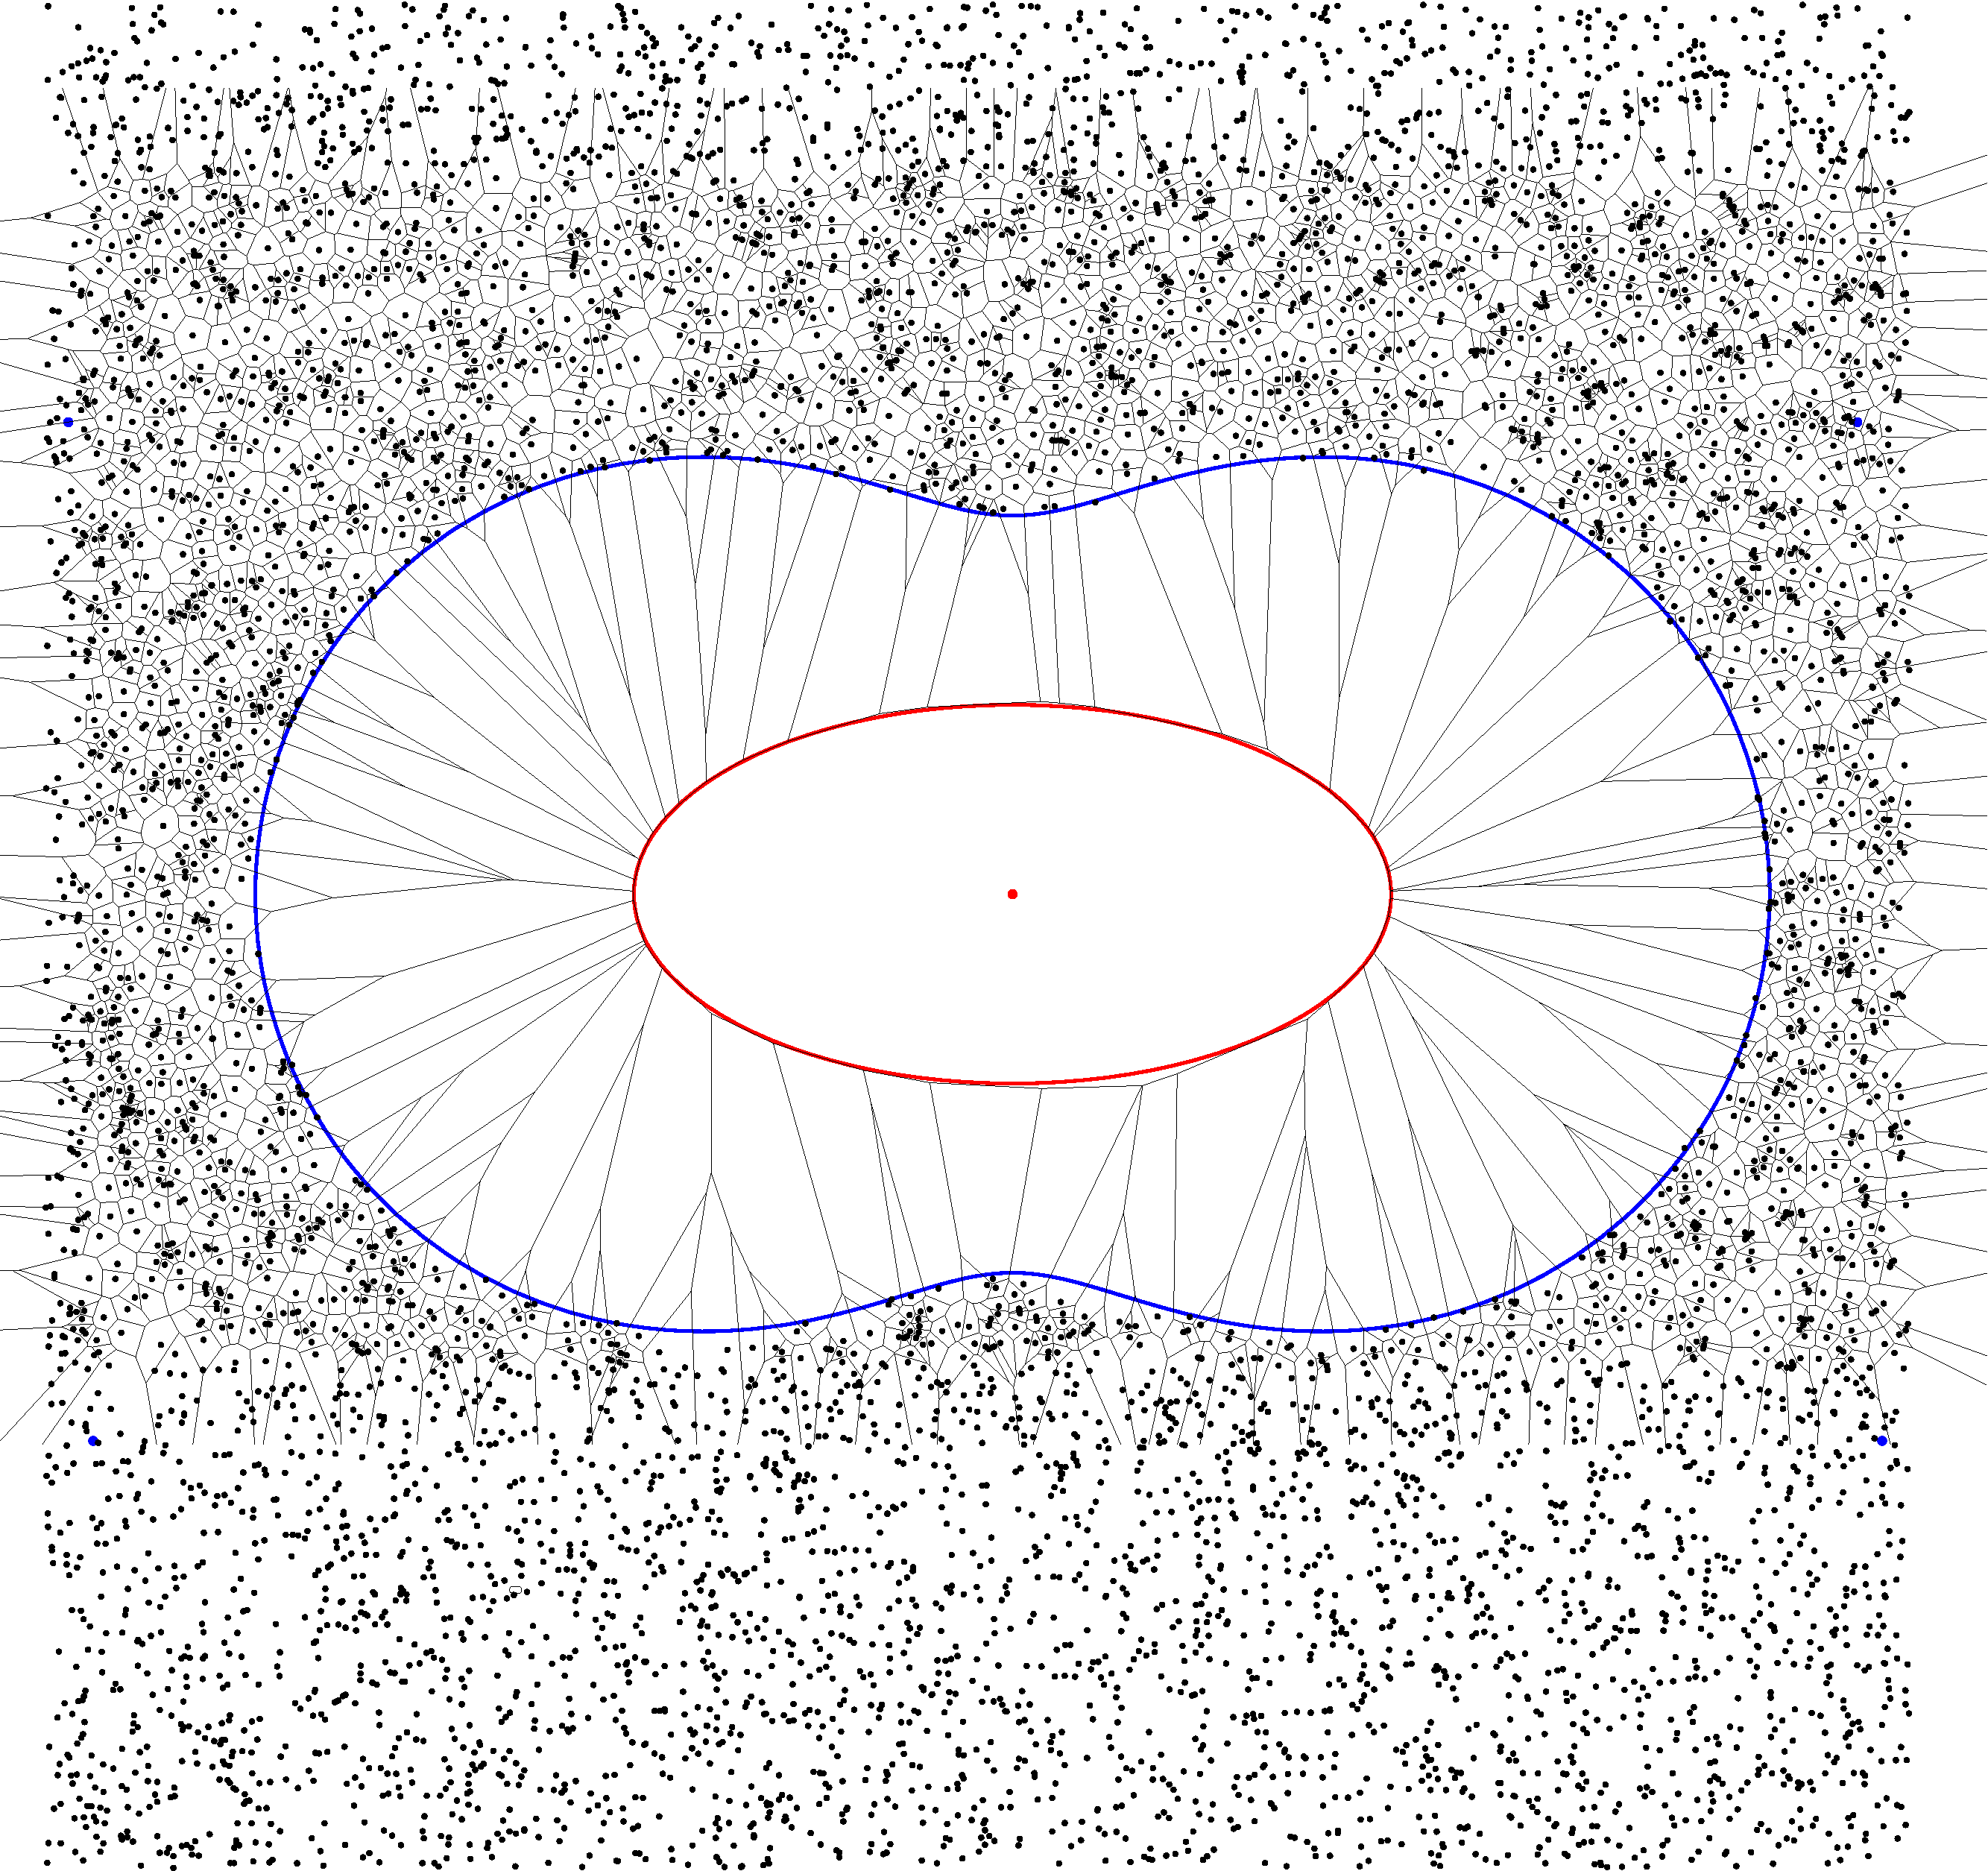
\includegraphics[trim= 3.5cm 11.5cm 3cm 6cm, clip, scale=0.2]{simuapproxellipse.pdf}
\hspace*{1cm}
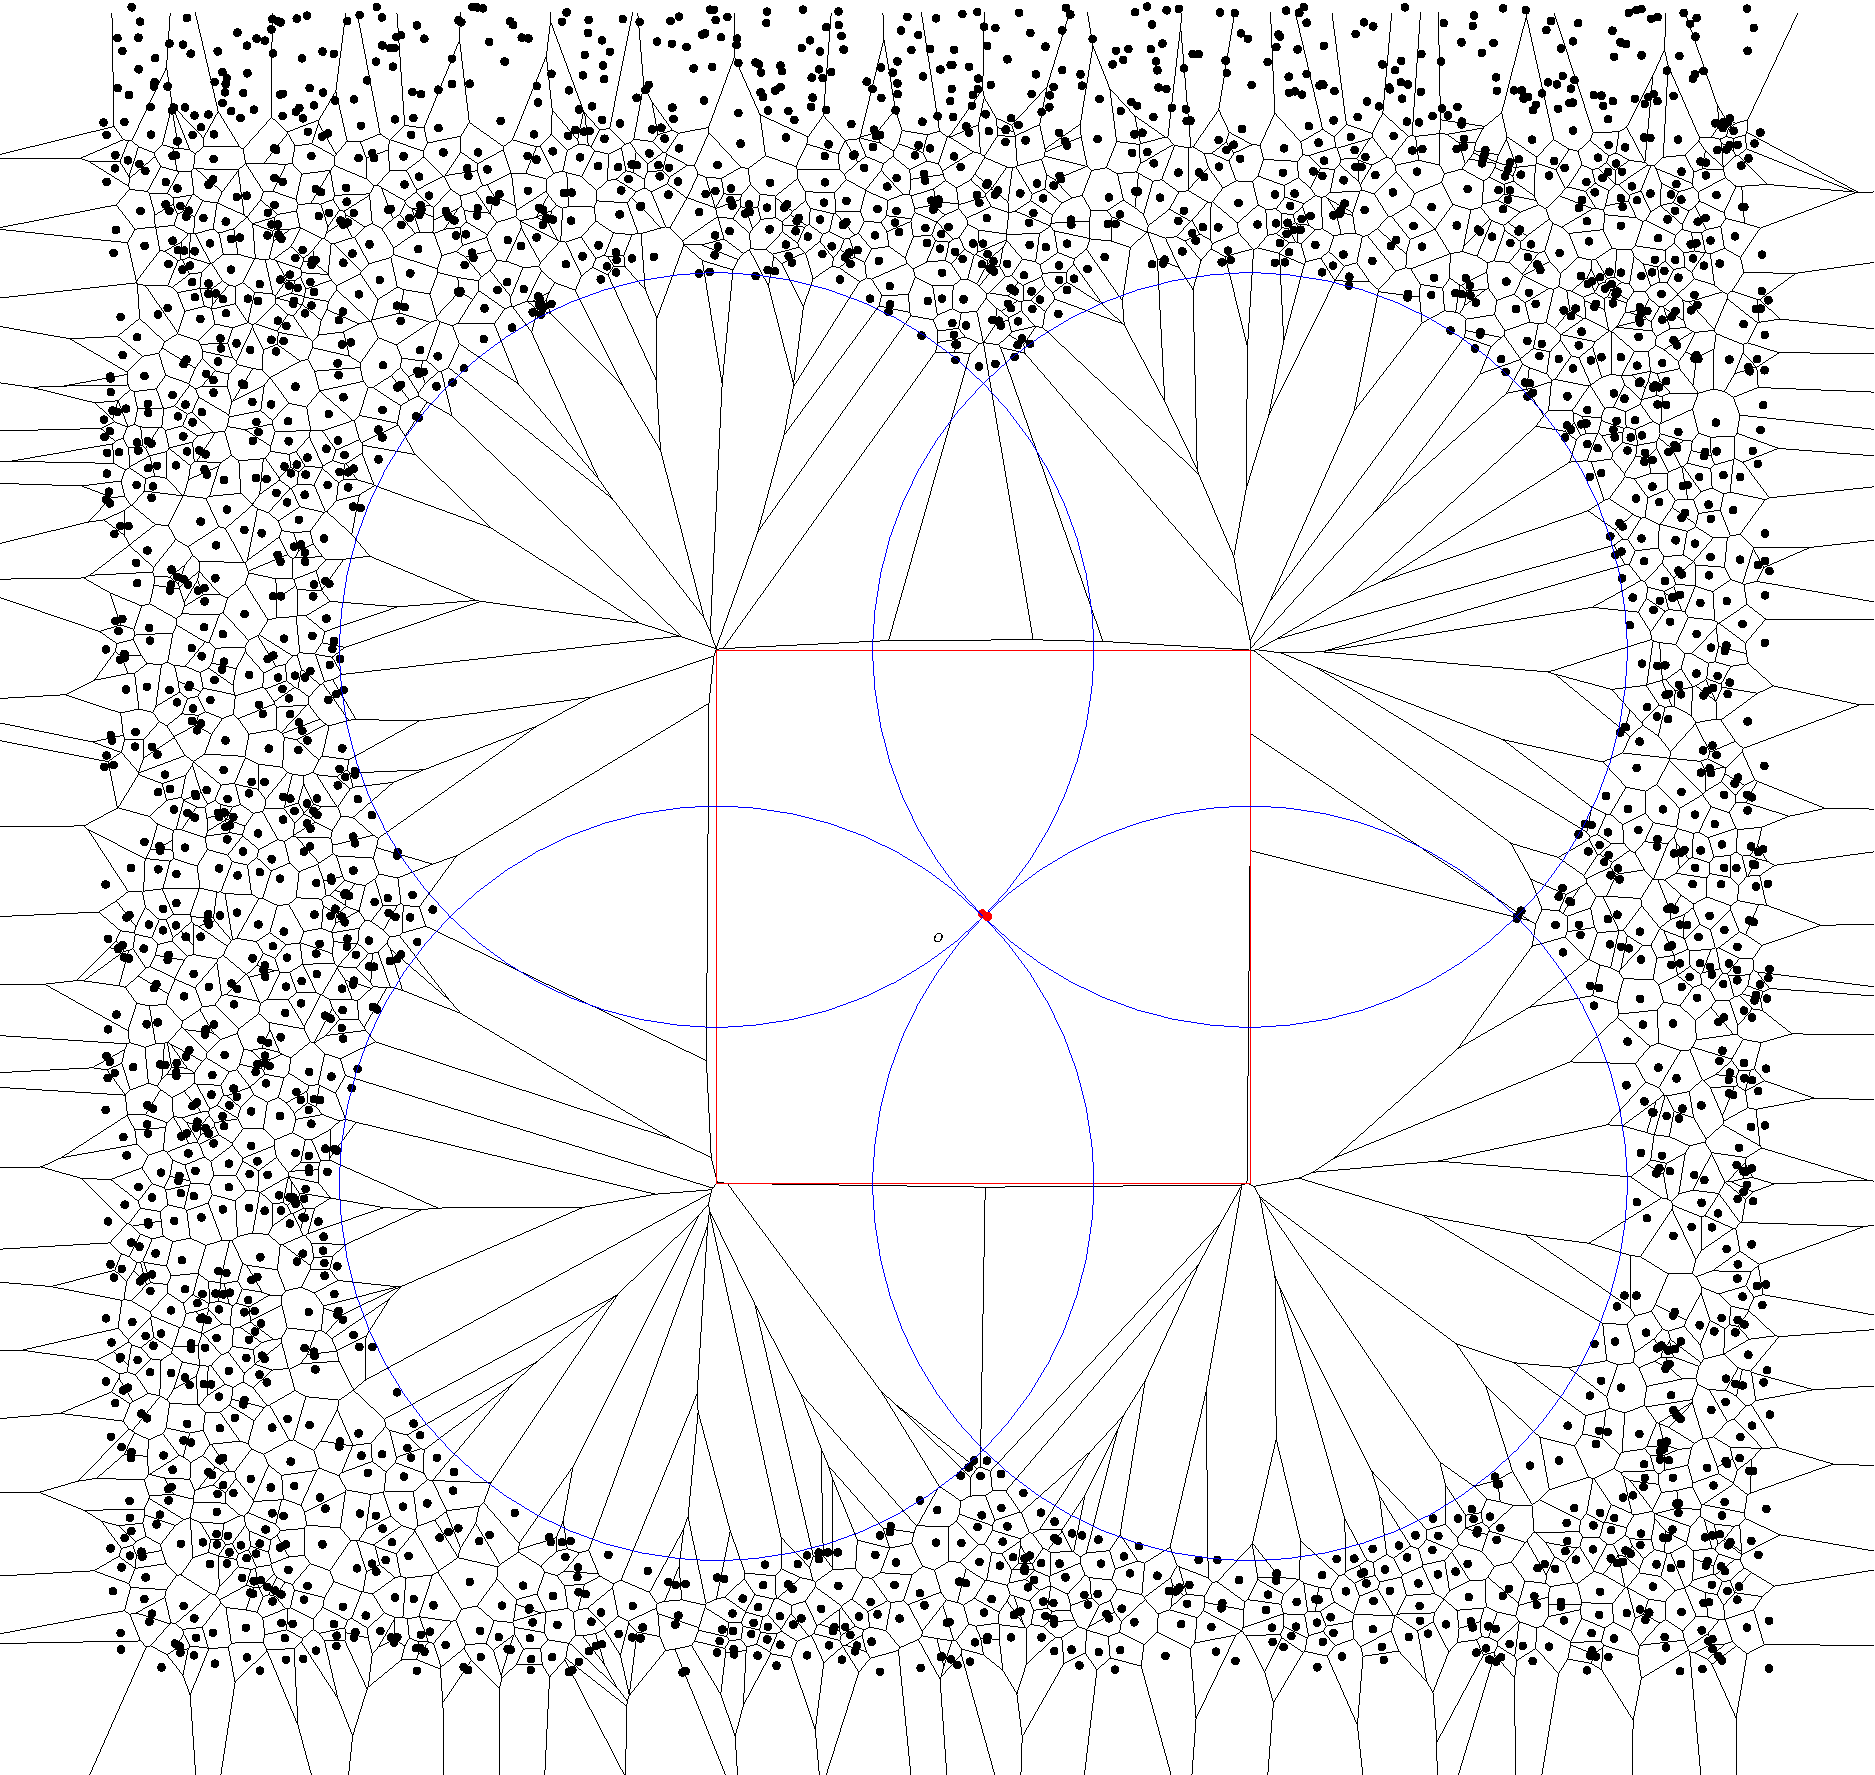
\includegraphics[trim= 3.5cm 2.5cm 3cm 3cm, clip, scale=0.205]{simuapproxcarre.pdf}
\end{center}
\caption{Voronoi cells (red) generated by the origin and a Poisson point process of intensity $10000$ outside the double of the Voronoi flower (blue), with respect to the origin, of an ellipse (left) and of a square (right).}\label{fig:question2}
\end{figure}

%\pass
In a second step, we go back to the original problem, i.e. studying the asymptotic mean characteristics of the initial random polygon $K_{\lambda}$. We show that when $\lambda\to \infty$, the nucleus of $K_{\lambda}$ concentrates around a point whose associated Voronoi flower has the smallest area. This point is known as the Steiner point of $K$. Consequently, we derive in Theorem~\ref{theo:steiner} below the required asymptotic results for the mean characteristics of $K_{\lambda}$.

\begin{theo}\label{theo:steiner}
Let $K$ be a convex body with non-empty interior and with its Steiner point at the origin. The asymptotics of $\E(\cA({K}_\lambda))-\cA(K)$, $\E(\cU({K}_\lambda))-\cU(K)$ and $\E(\cN({K}_\lambda))$ are then provided by Theorem~\ref{theosmooth} when $K$ is smooth and by Theorem~\ref{theopolygon} when $K$ is a polygon.
\end{theo}

%\pass
The convergence in mean to zero of the defect area of $K_\lambda^o$ (resp. $K_\lambda$) allows us to show that both random polygons converge in probability to $K$ for the Hausdorff distance. Indeed since $K_\lambda^o$ (resp. $K_\lambda$) is a convex body which contains $K$, any tail probability of the Hausdorff distance between $K$ and $K_\lambda^o$ (resp. $K_\lambda$) is bounded by a tail probability of the defect area which in turn is upper-bounded by its expectation up to a multiplicative constant, thanks to Markov's inequality. Moreover, when the processes ${\cP}_\lambda$, $\lambda>0$, are coupled, the convergence holds almost surely. The results are stated in Corollary~\ref{cor:bonustrack} below.

\begin{coro}\label{cor:bonustrack}
Let ${\cP}$ be the homogeneous Poisson point process of intensity $1$ in $\R^3$. When ${\cP}_\lambda=\{x\in\R^2:\exists t\in (0,\lambda) \text{ such that } (x,t)\in \cP\}$, the random polygons $K_\lambda^o$ and $K_\lambda$ converge almost surely to $K$ for the Hausdorff distance when $\lambda\to\infty$.
\end{coro}

%\pass
We also collect further results in two directions. First, we obtain explicit limiting variances in the smooth case for the defect area and the number of vertices. The results are provided in Theorem~\ref{theo:var} below.


\begin{theo}\label{theo:var}
Let $K$ be a smooth convex body. There exists two positive constants $c_{\cA}$ and $c_{\cN}$, independent of $K$, such that the variances of the defect area and the number of vertices of $K_{\lambda}^o$ have respectively the following asymptotics when the intensity $\lambda\to\infty:$
\begin{align}
\tag{$\rm i$}\label{theo1.5.i} &\emph{Var}(\cA(K_{\lambda}^o))\underset{\lambda\to\infty}{\sim}\lambda^{-\frac{5}{3}}2^{-\frac{13}{3}}\pi^{-1}c_{\cA}\int_{\partial K} r_s^{\frac4{3}}\left\langle s,n_s\right\rangle^{-\frac{5}{3}}\dd s\\
\tag{$\rm ii$}\label{theo1.5.ii} &\emph{Var}(\cN(K_{\lambda}^o))\underset{\lambda\to\infty}{\sim}\lambda^{\frac{1}{3}}2^{-\frac{1}{3}}\pi^{-1}c_{\cN}\int_{\partial K} r_s^{-\frac{2}{3}}\left\langle s,n_s\right\rangle^{\frac1{3}}\dd s.
\end{align}
\end{theo}


%\pass
These results are on par with the explicit limiting variances which were obtained in~\cite{cy14} for the number of $k$-dimensional faces and volume of random convex hulls inside a smooth convex body. It comes as no surprise as the proof of Theorem~\ref{theo:var} relies on a polarisation argument followed by a general technique already used in~\cite{cy14}. In both models, the growth rate of the variance of each functional coincides with the rate of its expectation. The case of the perimeter seems more intricate and is briefly discussed at the end of Section~\ref{sec:variancesmooth}.

%\pass
Second, analogues of Theorems~\ref{theosmooth} and~\ref{theopolygon} are derived when the Poisson--Voronoi cell is replaced by the so-called Crofton cell.

%\pass
The paper is structured as follows. We start by presenting in Section~\ref{sec:keytools} preliminary results related to the so-called support function of $K_{\lambda}^o$. The proofs of Theorems~\ref{theosmooth} and~\ref{theopolygon} are presented in Section~\ref{sec:smooth} and Section~\ref{sec:polygon} for the smooth and polygonal cases respectively. The answers to the original question are summarized in Section~\ref{sec:steiner}. In Section~\ref{sec:variancesmooth}, the additional results on the limiting variances are proved and followed by a general discussion on possible extensions of the method. Finally, Section~\ref{sec:crofton} contains the proofs for the analogues of the limiting expectations for the Crofton cell.



\section{The key role of the support function}\label{sec:keytools}

%\noi
In this section, we rewrite in a tractable way the three expectations which appear in Theorems~\ref{theosmooth} and~\ref{theopolygon}, i.e. we aim at getting the three relations~\eqref{eq:airesmooth}, \eqref{eq:croftonperimeter} and~\eqref{eq:efronvertices}. We also emphasize the basic ideas and guidelines of the proofs from Sections~\ref{sec:smooth} and~\ref{sec:polygon}.

%\pass
Let us introduce the Voronoi flower of a compact set $L$ with respect to a point $x\in\R^2$ as the set defined by
\begin{equation}\label{def:vorflow}
\cF_x(L)= \bigcup_{s\,\in\,L} B_{\frac1{2}\|s-x\|}\left(\tfrac1{2}(s+x)\right)
\end{equation}
where $B_r(z)$ denotes the closed ball centered at $z\in \R^2$ and of radius $r\ge 0$. This set is central in the study of Voronoi tessellations for the reasons described below and has sometimes been renamed as the \emph{fundamental region}, see e.g.~\cite{zuyev}. A quick study of the literature reveals that in most cases the set $2\cF_x(L)$ instead of $\cF_x(L)$ is considered. We have chosen this arbitrary normalization of the Voronoi flower in this work in order to connect it to the notion of pedal curve, see e.g.~\cite[Chapter~11]{zwikker}. In other words, the boundary of $\cF_x(L)$ is the pedal curve associated with the boundary of $L$ with respect to the pedal point at $x$.

%\pass
We notice in particular that $\cF_x(L)=\cF_x(\conv(L))$ where $\conv(\cdot)$ denotes the convex hull. The basic equivalence
\begin{equation*}\label{eq:loipoissfleur}
x\in K_{\lambda}^o\setminus K \Longleftrightarrow \cP_{\lambda}\cap 2\big(\cF_o(K\cup \{x\})\setminus \cF_o(K)\big)=\emptyset
\end{equation*}
and the equality
\begin{equation}\label{eq:emptycap}
\P\big(\cP_{\lambda}\cap 2(\cF_o(K\cup \{x\})\setminus \cF_o(K)\big) = \emptyset = \exp\big(-4\lambda\cA(\cF_o(K \cup \{x\})\setminus\cF_o(K))\big)
\end{equation}
imply that
\begin{equation}\label{eq:airesmooth}
\E(\cA(K_{\lambda}^o))-\cA(K) = \int_{\R^2\setminus K} \exp\big(-4\lambda\cA(\cF_o(K \cup \{x\})\setminus\cF_o(K))\big)\dd x.
\end{equation}

%\noi
Thus, our problem consists in providing accurate estimates for the extra area of the Voronoi flower of $K$ when adding to $K$ a single point $x$ outside of it. We will need to treat separately the case where $K$ has a smooth boundary (Lemma~\ref{lem:geom}) and the case where $K$ is a convex polygon (Lemma~\ref{lem:geompoly1}). In particular, Lemma~\ref{lem:geom} will be proved using the Cauchy--Crofton formula~\eqref{eq:formuleairefleur} involving the so-called support function of $K$.

%\pass
For every $\theta\in [0,2\pi)$, let us denote by $(u_{\theta},v_{\theta})$ the orthonormal basis in direction $\theta$, i.e. $u_{\theta}=(\cos\theta,\sin\theta)$ and $v_{\theta}=(-\sin\theta,\cos\theta)$. The support function of $K$ with respect to a point $x\in\R^2$ (see e.g.~\cite[Section~1.7]{Schneider}) is the function defined for $z\in\R^2$ by
\begin{equation*}\label{def:suppfunc}
p_x(K,z) = \sup_{y\,\in\,K}\langle y-x,z\rangle.
\end{equation*}

%\noi
Observe that $p_x(K,\cdot)$ is homogeneous of degree~$1$. We will denote by $p_x(K,\theta)$ the quantity $p_x(K,u_\theta)$ and we will use indifferently both notations in the sequel, depending on the context. In particular, when $x\in K$, the distance from $x$ to the boundary of $\cF_x(K)$ in direction $u_{\theta}$ is precisely $p_{x}(K,\theta)$, which implies in turn that
\begin{equation}\label{eq:formuleairefleur}
\cA(\cF_x(K))=\frac1{2}\int_0^{2\pi}p^2_x(K,\theta)\dd \theta.
\end{equation}

%\pass
The support function also makes it possible to rewrite the defect perimeter as an integral using the well-known Cauchy--Crofton formula
\begin{equation}\label{eq:croftonperimeter}
\E(\cU(K_{\lambda}^o))-\cU(K)=\int_0^{2\pi} \E(p_o(K_{\lambda}^o,\theta)-p_o(K,\theta))\dd\theta.
\end{equation}

%\noi
Therefore, in order to deal with this expectation we aim to determine the distribution of the point which achieves the support function into a fixed direction (see Propositions~\ref{prop:supportsmooth} and~\ref{prop:supportpoly}). The strategy will consist in using nontrivial changes of variable according to the case where $K$ is smooth or not. The main difficulty will be in the computation of its Jacobian, the determination of the domain of integration for it and finally its integration.

%\pass
In the next proposition, we prove a relation in the same spirit as the well-known Efron's relation for convex hulls of random inputs, see e.g.~\cite{Efron}, which connects the mean number of sides of $K_{\lambda}^o$ either to the mean defect area of the flower or to the mean defect support function. Efron-type identities for random tessellations have been recently derived in~\cite[Section~5]{Sch09} and~\cite[Theorem~3.1]{hhrt}. The two formulas below are new though the method to get~\eqref{prop2.1.i} is very similar to these two references. Only the asymptotic relation~\eqref{eq:efronvertices} will be used in the sequel.

\begin{prop}\label{prop:efron}\ \\*[-1.4em]
%\noi
\begin{enumerate}\romanenumi
\item \label{prop2.1.i}For every $\lambda>0$, the following identity holds
\begin{equation*}
\E(\cN(K_{\lambda}^o)) = 4\lambda \big(\E\big(\cA(\cF_o(K_{\lambda}^o))-\cA(\cF_o(K))\big)\big).
\end{equation*}
\item \label{prop2.1.ii}Moreover,
\begin{equation}\label{eq:efronvertices}
\E(\cN(K_{\lambda}^o))= 4\lambda\int_0^{2\pi}p_o(K,\theta)\E(p_o(K_{\lambda}^o,\theta)-p_o(K,\theta))\dd\theta+{\cR}_\lambda
\end{equation}
where ${\cR}_\lambda=2\lambda\int_0^{2\pi}\E\left((p_o(K_{\lambda}^o,\theta)-p_o(K,\theta))^2\right)\dd\theta$.
\end{enumerate}
\end{prop}

\begin{proof}[{Proof of Proposition~\ref{prop:efron}}]
We recall that $\cN(K_{\lambda}^o)$ is the number of neighbors of $o$, i.e. the set of all $x\in\cP_{\lambda}\setminus 2\cF_o(K)$ such that the bisecting line of the segment $[o,x]$ has a non-empty intersection with the boundary of $K_{\lambda}^o$. Moreover, for any $x\in\cP_{\lambda}\setminus 2\cF_o(K)$, $x$ is a neighbor of $o$ if and only if $\tfrac{1}{2}x\in \cF_o(C_x)\setminus\cF_o(K)$, where $C_x$ is the Voronoi cell of the origin associated with the set of nuclei $(\cP_{\lambda}\setminus 2\cF_o(K))\setminus\{x\}$. Consequently, thanks to Mecke--Slivnyak's formula (see~\cite[Corollary~3.2.3]{SW}) and Fubini theorem, we obtain
\begin{align*}
\E(\cN(K_{\lambda}^o)) &= \E\bigg(\sum_{x\,\in\,\cP_{\lambda}\setminus2\cF_o(K)}{\emph{\indicat}}_{\left\{\frac{x}{2}\,\in\,\cF_o(C_x)\,\setminus\,\cF_o(K)\right\}}\bigg)\\
& = \lambda\int_{\R^2\,\setminus\,2\cF_o(K)}\P\big(x\in 2(\cF_o(K_{\lambda}^o)\setminus\cF_o(K))\big)\dd x \\
& = 4\lambda\E\big(\cA(\cF_o(K_{\lambda}^o))-\cA(\cF_o(K))\big).
\end{align*}

%\noi
Now, using~\eqref{eq:formuleairefleur}, we obtain
\begin{multline*}\label{sophie}
\E(\cN(K_{\lambda}^o)) \\
\begin{aligned}
& = 2\lambda\int_0^{2\pi}\E\left(p_o^2\left(K_{\lambda}^o,\theta\right)-p_o^2(K,\theta)\right)\dd\theta\\
& = 2\lambda\int_0^{2\pi}\E\big((2p_o(K,\theta)+(p_o(K_{\lambda}^o,\theta)-p_o(K,\theta)))(p_o(K_{\lambda}^o,\theta)-p_o(K,\theta))\big)\dd\theta.
\end{aligned}
\end{multline*}
This completes the proof of Proposition~\ref{prop:efron}.
\end{proof}

%\pass
Let us notice that Proposition~\ref{prop:efron} can be extended to higher dimension when the number of sides is replaced by the number of facets.

%\pass

We now rewrite Proposition~\ref{prop:efron} in the two particular cases when $K$ has a smooth boundary (Corollary~\ref{coro:appliEfronsmooth}) and when $K$ is a convex polygon (Corollary~\ref{coro:appliEfronpolygonal}). We will show in both cases that the first term in the right hand side of~\eqref{eq:efronvertices} is the leading term while the quantity ${\cR}_\lambda$ is negligible.

\begin{coro}\label{coro:appliEfronsmooth}
If $K$ has a smooth boundary, then
\begin{equation}\label{coro2.2.1}
\E(\cU(K_{\lambda}^o))-\cU(K)=\int_{\partial K} \E(Y_{s,\lambda})r_s^{-1} \dd s \tag{$\rm i$}
\end{equation}
\begin{equation}\label{coro2-2.2}
\E(\cN(K_{\lambda}^o))= 4\lambda\int_{\partial K}\langle s,n_s\rangle\E(Y_{s,\lambda})r_s^{-1}\dd s+{\cR}_\lambda \tag{$\rm ii$}
\end{equation}
where $Y_{s,\,\lambda}= p_o(K_{\lambda}^o,n_s)-p_o(K,n_s)$ and ${\cR}_\lambda=2\lambda\int_{\partial K}\E(Y_{s,\lambda}^2)r_s^{-1}\dd s$.
\end{coro}

\begin{proof}[{Proof of Corollary~\ref{coro:appliEfronsmooth}}]
%\noi
When $K$ has a smooth boundary, for every $s\in \partial K$ such that $n_s=u_\theta$, we get
\begin{equation*}\label{eq:chgtsr}
\frac{\dd s}{\dd \theta}=r_s\,\text{ and }\, p_o(K,\theta)=p_o(K,n_s)=\langle s,n_s\rangle.
\end{equation*}
We obtain the two results by setting $Y_{s,\lambda}= p_o(K_{\lambda}^o,n_s)-p_o(K,n_s)$ and applying~\eqref{eq:croftonperimeter} and Proposition~\ref{prop:efron}$\MK$\eqref{prop2.1.ii}.
\end{proof}

%\pass
Let us now rewrite Proposition~\ref{prop:efron} when $K$ is a polygon. Let us denote by $u_{\delta_i}$, $\delta_i\in (0,2\pi)$, the external unit normal vector to the line $(a_{i},a_{i+1})$ (with the convention $\delta_0=\delta_{n_K}$). We expect $\E(p_o(K_{\lambda}^o,\theta)-p_o(K,\theta))$ to be maximal in directions \emph{close} to $\delta_i$ for every $i$ while the remaining directions should have a negligible contribution inside the integrals on the right-hand side of~\eqref{eq:croftonperimeter} and~\eqref{eq:efronvertices}.

\begin{coro}\label{coro:appliEfronpolygonal}
If $K$ is a convex polygon, then
\begin{align}
\tag{$\rm i$}\label{coro2.3.1} &\E(\cU(K_{\lambda}^o))-\cU(K) = \sum_{i=1}^{n_K}\,\int_{\eta_{i,\lambda}}^{\infty}\,\sum_{\varepsilon\,\in\,\{+,-\}} \E\left(Z_{i,\gamma,\lambda,\eps}\right)(\lambda^{-\gamma}\log \lambda)\dd\gamma \\
\tag{$\rm ii$}\label{coro2.3.2}  &\E(\cN(K_{\lambda}^o))\\
&= 4\lambda\sum_{i=1}^{n_K}\,\int_{\eta_{i,\lambda}}^{\infty}\,\sum_{\varepsilon\,\in\,\{+,-\}}p_o\left(K,\delta_i+\varepsilon\lambda^{-\gamma}\right)
\E(Z_{i,\gamma,\lambda,\eps})\left(\lambda^{-\gamma}\log\lambda\right)\dd\gamma+{\cR}_\lambda\nonumber
\end{align}
where
\begin{align*}
\eta_{i,\lambda}&=-\frac{\log \left(\frac{1}{2}(\delta_i-\delta_{i-1})\right)}{\log\lambda},\\
Z_{i,\gamma,\lambda,\eps}&= p_o\left(K_{\lambda}^o,\delta_i+\varepsilon\lambda^{-\gamma}\right)-p_o\left(K,\delta_i+\varepsilon\lambda^{-\gamma}\right)
\end{align*}
and
\begin{equation}\label{eq:defRlambdapolyg}
{\cR}_\lambda=2\lambda \sum_{i=1}^{n_K} \int_{\eta_{i,\lambda}}^{\infty} \sum_{\varepsilon\,\in\,\{+,-\}}\,\E\,\left(Z_{i,\gamma,\lambda,\eps}^2\right)\left(\lambda^{-\gamma}\log \lambda\right)\dd\gamma.
\end{equation}
\end{coro}

\begin{proof}[{Proof of Corollary~\ref{coro:appliEfronpolygonal}.}]

\begin{prooff}[{Proof of~\eqref{coro2.3.1}}]
The integral in~\eqref{eq:croftonperimeter} is equal to
\[
\sum_{i=1}^{n_K} \bigg(\int_{\delta_{i-1}}^{\frac1{2}\left(\delta_{i-1}+\delta_{i}\right)} \E\big(p_o(K_{\lambda}^o,\theta)-p_o(K,\theta)\big)\dd\theta + \int_{\frac1{2}\left(\delta_{i-1}+\delta_{i}\right)}^{\delta_{i}} \E\big(p_o(K_{\lambda}^o,\theta)-p_o(K,\theta)\big)\dd\theta\bigg).
\]

%\noi
Let us only estimate the second integral above (the first one will be treated analogously). Using the change of variable $\theta=\delta_i-\lambda^{-\gamma}$, we get
\begin{equation*}\label{eq:perimpolyginterm0}
\int_{\frac1{2}\left(\delta_{i-1}+\delta_i\right)}^{\delta_i} \E(p_o(K_{\lambda}^o,\theta)-p_o(K,\theta))\dd\theta = \int_{\eta_{i,\lambda}}^{\infty} \E(Z_{i,\gamma,\lambda,-})(\lambda^{-\gamma}\log \lambda)\dd\gamma.
\end{equation*}
\end{prooff}
%\noi
\begin{lastprooff}[{Proof of~\eqref{coro2.3.2}}]
This point is stated in the same way by decomposing the integral in~\eqref{eq:efronvertices} and using the same changes of variables.
\end{lastprooff}\let\qed\relax
\end{proof}
%$\square$



\section{The smooth case}\label{sec:smooth}

%\noi
In this section, $K$ is a smooth convex body containing the origin in its interior. Every $x\in\R^2\setminus K$ can be written as $x=s+hn_s=s_h$ with $s\in\partial K$ and $h>0$. We denote by $\Delta\cF_{s_h}$ the set $\cF_o(K\cup \{s_h\})\setminus \cF_o(K)$. Because of~\eqref{eq:emptycap} and~\eqref{eq:airesmooth}, a key ingredient for proving Theorem~\ref{theosmooth} is the estimate of the area $\cA(\Delta\cF_{s_h})$ of the increase $\Delta \cF_{s_h}$ of a Voronoi flower of $K$ induced by the addition of a point outside $K$. To the best of our knowledge this estimate stated in Subsection~\ref{subsec:fleursmooth} is new despite the natural aspect of the question. Subsections~\ref{subsec:surfacesmooth}, \ref{sub:perimetersmooth} and~\ref{subsec:verticessmooth} are then devoted to the asymptotic mean area of $K_{\lambda}^o$, the asymptotic mean support function and perimeter of $K_{\lambda}^o$ and the asymptotic intensity and mean number of vertices of $K_{\lambda}^o$ respectively.


\subsection{Increase of the area of the Voronoi flower}\label{subsec:fleursmooth}

%\pass

%\noi
The next lemma provides the exact calculation of the limiting rescaled defect area of the Voronoi flower as well as a lower-bound.

\begin{lemm}\label{lem:geom}
Let us assume that $K$ is a smooth convex body containing the origin $o$ in its interior.
\begin{enumerate}\romanenumi
\item \label{estimeevolfleur}For every $s\in\partial K$, we get
\begin{equation*}
\cA(\Delta\cF_{s_h})\underset{h\to 0}{\sim} h^{\frac{3}{2}} 2^{\frac{5}{2}}3^{-1}r_s^{-\frac1{2}}\langle s, n_s\rangle.
\end{equation*}
\item \label{eq:minorantvol}Moreover, there exists $C>0$ such that, for every $h>0$ and $s\in\partial K$,
\begin{equation*}
h^{-\frac{3}{2}}\cA(\Delta\cF_{s_h}) \ge C >0.
\end{equation*}
\end{enumerate}
\end{lemm}

%\noi
\begin{proof}[{Proof of Lemma~\ref{lem:geom}.}]
\begin{prooff}[{Proof of~\eqref{estimeevolfleur}}]
We wish to use the simpler case where the origin $o$ coincides with the center of curvature $\omega_s$ of $\partial K$ at point $s$. In other words, our aim is to show that the area $\cA(\Delta\cF_{s_h})$ can be calculated as a function of $\cA(\Delta\widetilde{\cF}_{s_h})$ where
\[
\Delta\widetilde{\cF}_{s_h}=\cF_{\omega_s}(K \cup \{s+h n_s\})-\cF_{\omega_s}(K).
\]

%\noi
We assume for the time being that $\omega_s$ belongs to $K$ and we will explain at the end of the proof how to adapt the arguments to the general case. We then use the equality~\eqref{eq:formuleairefleur} and the relation $p_x(K,\theta) -p_o(K,\theta) = -\langle x, u_{\theta}\rangle$ for every $x\in\R^2$, to obtain
\begin{equation}\label{eq:eqsuppl}
\cA(\cF_o(K)) =
\cA(\cF_{\omega_s}(K)) +\frac1{2}\int_0^{2\pi}\langle \omega_s, u_{\theta}\rangle^2\dd \theta+\int_0^{2\pi}p_{\omega_s}(K,\theta)\langle \omega_s, u_{\theta}\rangle\dd \theta.
\end{equation}

%\noi
Applying this formula to both $K$ and $K\cup\{s_h\}$ yields
\begin{equation}\label{eq:chaslesvol}
\cA(\Delta\cF_{s_h})=\cA(\Delta\widetilde{\cF}_{s_h}) + \int_0^{2\pi} \Delta p_{\omega_s}(\theta)\langle \omega_s, u_{\theta}\rangle\dd\theta
\end{equation}
where $\Delta p_{\omega_s}(\theta)=p_{\omega_s}(K \cup \{s_h\},\theta)-p_{\omega_s}(K, \theta)$.

%\pass
 We treat separately the two terms of the right-hand side of~\eqref{eq:chaslesvol}.

%\pass Step ?
$-$ \emph{Estimate of $\cA(\Delta\widetilde{\cF}_{s_h})$}.

%\noi
Let us define $s(\theta)$ as the point belonging to $\partial K$ such that $\theta \in(-\pi,\pi]$ is the angle between the two half-lines $\omega_s+\R_+(s-\omega_s)$ and $\omega_s+\R_+(s(\theta)-\omega_s)$ (see Figure~\ref{fig:geolemproof2}). Denote by $-\theta_{s,h}^-$ and $\theta_{s,h}^+$ the two angles such that $p_{\omega_s}(K\cup\{s_h\},\theta) = p_{\omega_s}(K,\theta)$ if and only if $\theta\notin[-\theta_{s,h}^-,\theta_{s,h}^+]$. Then we can write
\begin{equation}\label{eq:voldifflow1}
\cA(\Delta\widetilde{\cF}_{s_h})= \int_{-\theta_{s,h}^-}^{\theta_{s,h}^+}\int_{p_{\omega_s}(K,\theta)}^{(r_s+h)\cos\theta} r \dd r \dd\theta.
\end{equation}

\begin{figure}[!h]
\begin{center}
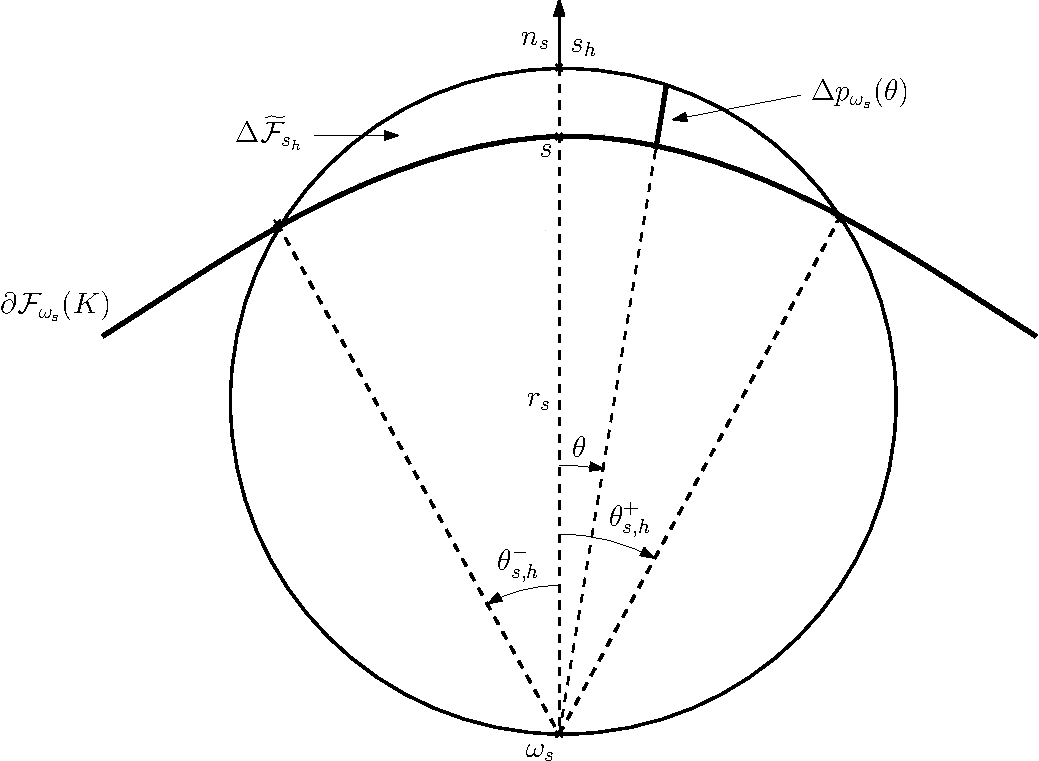
\includegraphics[scale=0.7]{geolemproof2.pdf}
\vspace{-0.0cm}
\caption{\label{fig:geolemproof2}
Flowers viewed from the center of curvature $\omega_s$ of $\partial K$ at point $s$.}
\end{center}
\end{figure}

%\noi
If $\partial K$ were a perfect circle of radius $r_s$ in the neighborhood of $s$ we would have $\theta_{s,h}^-=\theta_{s,h}^+=\theta_{s,h}$ with $\cos(\theta_{s,h})=\tfrac{r_s}{r_s+h}$. In particular, this means that when $h\to 0$,
\begin{equation}\label{eq:thetashequiv}
\theta_{s,h}^2\sim 2 r_s^{-1}h.
\end{equation}
In the general case, we approximate locally the polar equation of $\partial K$ with respect to the center $\omega_s$:
\begin{equation}\label{eq:s-omega}
\lim_{\theta\to 0}\theta^{-2}(\|s(\theta)-\omega_s\|-r_s)=0.
\end{equation}
Let us fix $\eta>0$. For $h>0$ small enough, we get from~\eqref{eq:s-omega}, \eqref{eq:thetashequiv} and the fact that $r_s$ is lower bounded along $\partial K$ that for any $s\in\partial K$ and $\theta\in [-\theta_{s,h}^-,\theta_{s,h}^+]$, $|\|s(\theta)-\omega_s\|-r_s|\le \eta h$. This implies that we can locally sandwich $\partial K$ between two circles of radii $r_s+\eta h$ and $r_s-\eta h$. This being true for any $\eta>0$, we deduce from this sandwiching that the angles $\theta_{s,h}^-$, $\theta_{s,h}^+$ and $\theta_{s,h}$ can all be written as
\begin{equation}\label{eq:angleaperture}
\theta_{s,h}^+\underset{h\to 0}{=}\theta_{s,h}^-+\od\left(h^{\frac{1}{2}}\right)\underset{h\to 0}{=}\theta_{s,h}+\od\left(h^{\frac{1}{2}}\right)
\underset{h\to 0}{=}2^{\frac1{2}}r_s^{-\frac{1}{2}}h^{\frac1{2}}+\od\left(h^{\frac{1}{2}}\right).
\end{equation}

%\noi
Moreover, since $\theta_{s,h}^+$ is bounded from above by its value obtained when $\partial K$ is replaced by an outer circle of radius $r_s+Ch$, we have
\begin{equation}\label{eq:dominationangleouverture}
\theta_{s,h}^+\le \arccos\left(1-\frac{h}{r_s+(C+1)h}\right)\le 2^{\frac1{2}}r_s^{-\frac1{2}}h^{\frac1{2}}.
\end{equation}

%\noi
Similarly, the defect of circularity implies that uniformly for $\theta\in [-\theta_{s,h}^-,\theta_{s,h}^+]$,
\begin{equation}\label{eq:defectcircularity}
p_{\omega_s}(K,\theta) \underset{h\to 0}{=} r_s+\od(h).
\end{equation}
Indeed, by definition of the curvature radius, $p_{\omega_s}(K,\theta)=r_s+\od(\theta^2)$ when $\theta\to 0$ and moreover, $\theta_{s,h}^{\pm}=\Odd(\theta^{\frac12})$ thanks to~\eqref{eq:angleaperture}.

%\noi
Let us show
\begin{equation}\label{eq:voldifflow2}
\cA\left(\Delta\widetilde{\cF}_{s_h}\right)\underset{h\to 0}{=}2^{\frac{5}{2}}3^{-1} r_s^{\frac1{2}}h^{\frac{3}{2}} + \od\left(h^{\frac32}\right).
\end{equation}

%\pass
Using~\eqref{eq:voldifflow1}, we get
\[
\cA\left(\Delta\widetilde{\cF}_{s_h}\right)= {\cA}^++{\cA}^-
\]
where
\[
\cA^+=\frac{(r_s+h)^2}{2}\left(\frac{\theta_{s,h}^+}{2}+\frac{\sin (2\theta_{s,h}^+)}{4}\right)-\int_0^{\theta_{s,h}^+}\frac{p_{\omega_s}^2(K,\theta)}{2}\dd\theta
\]
and $\cA^-$ is the same with $\theta_{s,h}^+$ replaced by $\theta_{s,h}^-$. In order to get~\eqref{eq:voldifflow2}, it is enough to show that when $h\to 0$,
\begin{equation}\label{eq:estimateA+}
\cA^+=2^{\frac32}3^{-1}r_s^{\frac12}h^{\frac32}+\od\left(h^{\frac32}\right)\;\;\text{ and } \;\;\cA^-=2^{\frac32}3^{-1}r_s^{\frac12}h^{\frac32}+\od\left(h^{\frac32}\right).
\end{equation}
We prove~\eqref{eq:estimateA+} for $\cA^+$ and omit the proof for $\cA^-$. We start by rewriting $\cA^+$ in a more appropriate way.
\begin{equation}\label{eq:rewritingA+}
\begin{aligned}
\cA^+&=\left(\frac{r_s^2}{2}+r_sh+\frac{h^2}{2}\right)\left[\theta_{s,h}^++\left(\frac{\sin(2\theta_{s,h}^+)}{4}-\frac{\theta_{s,h}^+}{2}\right)\right]\\
&\mkern160mu-\frac{1}{2} \int_0^{\theta_{s,h}^+}\left(p_{\omega_s}^2(K,\theta)-r_s^2\right)\dd\theta -\frac{r_s^2}{2}\theta_{s,h}^+
\\
&=T_1+T_2+T_3-T_4 
\end{aligned}
\end{equation}
where
\begin{align*}
T_1&=\frac{r_s^2}{2}\left(\frac{\sin (2\theta_{s,h}^+)}{4}-\frac{\theta_{s,h}^+}{2}\right),\\
T_2&=r_sh\theta_{s,h}^+,\\
T_3&=r_sh\left(\frac{\sin (2\theta_{s,h}^+)}{4}-\frac{\theta_{s,h}^+}{2}\right)+ \frac{h^2}{2}\left[\theta_{s,h}^++\left(\frac{\sin (2\theta_{s,h}^+)}{4}-\frac{\theta_{s,h}^+}{2}\right)\right],\\
T_4&=\frac{1}{2} \int_0^{\theta_{s,h}^+}\left(p_{\omega_s}^2(K,\theta)-r_s^2\right)\dd\theta.
\end{align*}
%%step4 ?
\noindent \emph{Study of $T_4$}: because of~\eqref{eq:defectcircularity}, $p_{\omega_s}(K,\theta)-r_s=\od(h)$ uniformly for $\theta\in [0,\theta_{s,h}^+]$ and
\[
p_{\omega_s}(K,\theta)^2-r_s^2=\Odd(p_{\omega_s}(K,\theta)-r_s)=\od(h).
\]
Integrating the estimate above, we obtain that when $h\to 0$
\begin{equation}\label{eq:estimT4}
T_4=\od\left(h\theta_{s,h}^+\right)=\od\left(h^{\frac32}\right).
\end{equation}


\noindent\emph{Study of $T_3$}: when $h\to 0$, $\theta_{s,\,h}^+\to 0$ so using~\eqref{eq:angleaperture}, we get when $h\to 0$
\begin{equation}\label{eq:estimdiffsin}
\frac{\sin (2\theta_{s,h}^+)}{4}-\frac{\theta_{s,h}^+}{2}= -\frac{8 {\theta_{s,h}^+}^3}{24}+\od\left({\theta_{s,h}^+}^3\right) = -2^{\frac32}3^{-1}r_s^{-\frac32}h^{\frac32}+\od\left(h^{\frac32}\right).
\end{equation}
This implies that
\begin{equation}\label{eq:estimT3}
T_3=\od\left(h^{\frac32}\right).
\end{equation}


\noindent\emph{Study of $T_2$}: using~\eqref{eq:angleaperture}, we get when $h\to 0$
\begin{equation}\label{eq:estimT2}
T_2=2^{\frac12}r_s^{\frac12}h^{\frac32}+\od\left(h^{\frac32}\right).
\end{equation}


\noindent\emph{Study of $T_1$}: using the estimate~\eqref{eq:estimdiffsin} above, we obtain that when $h\to 0$
\begin{equation}\label{eq:estimT1}
T_1=-2^{\frac12}3^{-1}r_s^{\frac12}h^{\frac32}+\od\left(h^{\frac32}\right).
\end{equation}
Inserting~\eqref{eq:estimT1}, \eqref{eq:estimT2}, \eqref{eq:estimT3} and~\eqref{eq:estimT4} into~\eqref{eq:rewritingA+}, we obtain the required result~\eqref{eq:estimateA+} and in turn~\eqref{eq:voldifflow2}.\\

%\pass
$-$ \emph{Estimate of $\int_0^{2\pi} \Delta p_{\omega_s}(\theta)\langle \omega_s, u_{\theta}\rangle\dd\theta$}.

%\pass
We have, uniformly for every $\theta\in[-\theta_{s,h}^-,\theta_{s,h}^+]$,
\[
\langle \omega_s, u_{\theta}\rangle \underset{h\to 0}{=} \langle \omega_s, n_s\rangle + \od(1).
\]

%\noi
Moreover, since $p_{\omega_s}(K\cup\{s_h\},\theta)= (r_s+h)\cos\theta$, we can write successively

\begin{align}
&\int_0^{2\pi} \Delta p_{\omega_s}(\theta)\langle \omega_s, u_{\theta}\rangle\dd\theta\nonumber\\
& \quad\; = \int_{-\theta_{s,h}^-}^{\theta_{s,h}^+} \Delta p_{\omega_s}(\theta)\langle \omega_s, u_{\theta}\rangle\dd\theta\nonumber\\
& \quad\underset{h\to 0}{=} (\langle \omega_s, n_s\rangle+\od(1))\int_{-\theta_{s,h}^-}^{\theta_{s,h}^+} \Delta p_{\omega_s}(\theta)\dd\theta\nonumber\\
&\quad \underset{h\to 0}{=} (\langle \omega_s, n_s\rangle+\od(1))\int_{-\theta_{s,h}^-}^{\theta_{s,h}^+} ((r_s+h)\cos\theta-r_s)\dd\theta\nonumber\\
&\quad \underset{h\to 0}{=} (\langle \omega_s, n_s\rangle +\od(1))\big((r_s+h)\left(\sin\left(\theta_{s,h}^+\right)+\sin\left(\theta_{s,h}^-\right)\right)-r_s\left(\theta_{s,h}^++\theta_{s,h}^-\right)\big)\nonumber\\
& \quad \underset{h\to 0}{=} 2^{\frac{5}{2}}3^{-1}\, r_s^{-\frac1{2}} \langle \omega_s, n_s\rangle h^{\frac{3}{2}}+ \od\left(h^{\frac32}\right)\label{eq:2ndtermequation9}
\end{align}
where the last line is deduced from the penultimate one by methods similar to those used to prove statements~\eqref{eq:estimT4} to~\eqref{eq:estimT1}.\\

%\pass
 $-$ \emph{Conclusion when $\omega_s\in K$}.

%\noi
Inserting~\eqref{eq:voldifflow2} and~\eqref{eq:2ndtermequation9} into~\eqref{eq:chaslesvol} and using $s=\omega_s+r_s n_s$, we get
\begin{align*}
\cA(\Delta\cF_{s_h}) & \underset{h\to 0}{=} 2^{\frac{5}{2}}3^{-1} r_s^{\frac1{2}}\left(1+r_s^{-1}\langle \omega_s, n_s\rangle\right)h^{\frac{3}{2}} + \od\left(h^{\frac32}\right)\\
& \underset{h\to 0}{=} 2^{\frac{5}{2}}3^{-1} r_s^{-\frac1{2}}\langle s,n_s\rangle h^{\frac{3}{2}} + \od\left(h^{\frac32}\right)
\end{align*}
that gives the desired result.\\

%\pass regarder pour mettre des subsubsection ou des paragraph à la place de ces tirets ?
$-$ \emph{Case when $\omega_s\not\in K$}.

%\noi
The equality~\eqref{eq:eqsuppl} is still valid as soon as the term $\cA(\cF_{\omega_s}(K))$ in the right-hand side of~\eqref{eq:eqsuppl} is replaced by $\frac{1}{2}\int_0^{2\pi}p_{\omega_s}^2(K,\theta)\dd\theta$. Applying this new equality to both $K$ and $K\cup\{s_h\}$, we get that
\begin{equation}\label{eq:suppl2}
\cA(\Delta\cF_{s_h})=\frac{1}{2}\int_0^{2\pi}\left(p_{\omega_s}^2\left(K\cup\{s_h\},\theta\right)-p_{\omega_s}^2(K,\theta)\right)\dd\theta + \int_0^{2\pi} \Delta p_{\omega_s}(\theta)\langle \omega_s, u_{\theta}\rangle\dd\theta
\end{equation}
We claim that for $h>0$ small enough,
\begin{equation}\label{eq:suppl3}
\frac{1}{2}\int_0^{2\pi}\left(p_{\omega_s}^2(K\cup\{s_h\},\theta)-p_{\omega_s}^2(K,\theta)\right)\dd\theta=\cA\left(\Delta\widetilde{\cF}_{s_h}\right).
\end{equation}
Indeed, for $h>0$ small enough, the area $\cA(\Delta\widetilde{\cF}_{s_h})$ stays the same when $K$ is replaced by $K\cup\{\omega_s\}$. Moreover, on the left-hand side, we recall that $p_{\omega_s}(K\cup\{s_h\},\theta)= p_{\omega_s}(K,\theta)$ as soon as $\theta\not\in [-\theta_{s,h}^-,\theta_{s,h}^+]$ and when $\theta\in [-\theta_{s,h}^-,\theta_{s,h}^+]$, $p_{\omega_s}(K\cup\{s_h\},\theta)$ and $ p_{\omega_s}(K,\theta)$ stay the same when $K$ is replaced by $K\cup\{\omega_s\}$. Consequently, we can proceed as if $\omega_s$ would belong to $K$, which allows us to derive~\eqref{eq:suppl3} from~\eqref{eq:formuleairefleur}. Combining now~\eqref{eq:suppl2} and~\eqref{eq:suppl3}, we get~\eqref{eq:chaslesvol} and then Lemma~\ref{lem:geom}$\MK$\eqref{estimeevolfleur} by repeating verbatim the rest of the arguments.
\end{prooff}
%\pass


\begin{lastprooff}[{Proof of~\eqref{eq:minorantvol}}]
Thanks to~\eqref{estimeevolfleur}, the function which to any couple $(s,h)$ associates either
\[
\cA(\Delta\cF_{s_h})h^{-\frac{3}{2}}\text{ if }h>0\text{ or }2^{\frac52}3^{-1}r_s^{-\frac12}\langle s,n_s\rangle
\]
if $h=0$ is continuous on the compact set $\partial K\times [0,1]$ so it is bounded from below by a positive constant $C>0$. When $h\geq1$, we notice that the region $\Delta\cF_{s_h}$ contains a disk of radius proportional to $h$, which means that there exists $C'>0$ such that $\cA(\Delta\cF_{s_h})\geq C' h^2\geq C'h^{\frac{3}{2}}$.
\end{lastprooff}\let\qed\relax
\end{proof}


\subsection{Proof of Theorem~\ref{theosmooth}$\MK$\eqref{theo1.1.i}: the defect area}\label{subsec:surfacesmooth}

%\pass

%\noi
\begin{proof}[{Proof of Theorem~\ref{theosmooth}$\MK$\eqref{theo1.1.i}}]
Every $x\in\R^2\setminus K$ can be written as $x=s+\lambda^{-\frac{2}{3}}hn_s=s_{\lambda^{-\frac{2}{3}}h}$ with $s\in\partial K$ and $h>0$, the Jacobian of this change of variables being given by
\begin{equation*}\label{eq:jacobcurviligne}
\frac{\dd x}{\dd s \dd h} = \lambda^{-\frac{2}{3}}\left|1+\lambda^{-\frac{2}{3}}hr_s^{-1}\right|.
\end{equation*}

%\noi
Thus we get from~\eqref{eq:airesmooth} that
\[
\E(\cA(K_{\lambda}^o))-\cA(K) = \lambda^{-\frac{2}{3}}\int_{\partial K}\int_0^{\infty} \exp\left(-4\lambda \cA\left(\Delta\cF_{s_{\lambda^{-2/3}h}}\right)\right)\left|1+\lambda^{-\frac{2}{3}}hr_s^{-1}\right| \dd h \dd s.
\]

%\noi
Thanks to Lemma~\ref{lem:geom}, we get, for $h>0$ fixed,
\[
4\lambda \cA\left(\Delta\cF_{s_{\lambda^{-2/3}h}}\right) \underset{\lambda\to\infty}{\sim} 4\left(\lambda^{-2/3}h\right)^{-\frac{3}{2}} \cA\left(\Delta\cF_{s_{\lambda^{-2/3}h}}\right) h^{\frac{3}{2}} \underset{\lambda\to\infty}{\sim} C_s h^{\frac{3}{2}}
\]
where $C_s = 2^{\frac{9}{2}}3^{-1}r_s^{-\frac1{2}}\langle s,n_s\rangle $ and the existence of a constant $C>0$ such that, for all $\lambda>0$ and $s\in \partial K$,
\[
4\lambda \cA\left(\Delta\cF_{s_{\lambda^{-2/3}h}}\right) \ge C C_s h^{\frac{3}{2}}.
\]

%\noi
Consequently, we can apply Lebesgue's dominated convergence theorem to obtain
\[
\lambda^{\frac{2}{3}}(\E(\cA(K_{\lambda}^o))-\cA(K))
\underset{\lambda\to\infty}{\sim} \int_{\partial K}\int_0^{\infty} \exp\big(-C_s h^{\frac{3}{2}}\big) \dd h\dd s = \mfrac{2}{3}\Gamma\left(\frac{2}{3}\right)\int_{\partial K} C_s^{-\frac{2}{3}}\dd s
\]
which provides assertion~\eqref{theo1.1.i} of Theorem~\ref{theosmooth}.
\end{proof}
%$\square$


\subsection{Proof of Theorem~\ref{theosmooth}$\MK$\eqref{theo1.1.ii}: support points and defect perimeter}\label{sub:perimetersmooth}

%\pass

%\noi
The strategy of the proofs is to apply Corollary~\ref{coro:appliEfronsmooth} hence we only need now to explain how to estimate the mean defect support function in a fixed direction. To do so, let us introduce the support point $m_{s,\lambda}$ on $\partial K_{\lambda}^o$ in direction $n_s$, i.e. the point which satisfies $\langle m_{s,\lambda}, n_s\rangle=p_o(K_{\lambda}^o,n_s)$. Denoting by $X_{s,\lambda}=\langle m_{s,\lambda}-s,t_s\rangle$ and $Y_{s,\lambda}= p_o(K_{\lambda}^o,n_s)-p_o(K,n_s)$, we can write $m_{s,\lambda}=s+X_{s,\lambda}t_{s}+Y_{s,\lambda} n_s$ where $(t_s,n_s)$ stands for the Frenet frame at point $s$. Thus this subsection is devoted to investigate the asymptotic distribution of the couple $(X_{s,\lambda},Y_{s,\lambda})$ and provide the required asymptotic estimate for $\E(Y_{s,\lambda})$. A key step in the proof of Proposition~\ref{prop:supportsmooth} will the use of the following lemma providing a change of variables formula which may be understood as a classical formula \emph{à la} Blaschke--Petkantschin (see e.g.\cite[Theorem~7.3.1]{SW}). It consists essentially in the computation of the Jacobian of a four dimensional transformation. We omit the calculation which is analogous to the proof of the classical Blaschke--Petkantschin's formula (see the previous reference again).

%\goodbreak
\begin{lemm}\label{lem:jacob}
Let $x=r u_{\theta}$, $r>0$, $\theta\in (0,2\pi)$ and $\theta-\pi<\theta_1<\theta_2<\theta$. Let $x_1=2r\sin(\theta-\theta_1)u_{\theta_1+\frac{\pi}{2}}$ and $x_2=2r\sin(\theta-\theta_2)u_{\theta_2+\frac{\pi}{2}}$ be the symmetric points of the origin $o$ with respect to the lines $x+\R u_{\theta_1}$ and $x+\R u_{\theta_2}$ respectively. Then the Jacobian of the change of variables $(r,\theta,\theta_1,\theta_2)\longmapsto (x_1,x_2)$ is given by
\[
\frac{\dd x_1 \dd x_2}{r \dd r \dd \theta\dd \theta_1\dd \theta_2} = 16 r^2 J(\theta,\theta_1,\theta_2)
\]
with $J(\theta,\theta_1,\theta_2) = |\sin(\theta_1-\theta_2)\sin(\theta-\theta_2)\sin(\theta-\theta_1)|$.
\end{lemm}

\begin{prop}\label{prop:supportsmooth}\ \\*[-1.4em]
%\noi
\begin{enumerate}\romanenumi
\item \label{eq:ftheta}For every $s\in\partial K$, the couple $(\lambda^{\frac1{3}}X_{s,\lambda}, \lambda^{\frac{2}{3}}Y_{s,\lambda})$ converges in distribution when $\lambda\to\infty$ to the distribution with density function $f_s$ given by
\[
f_s(x,y)=2^{\frac{11}{2}}\langle s,n_s\rangle^2 r_s^{-\frac{3}{2}}\exp\left(-2^{\frac{9}{2}} 3^{-1}r_s^{-\frac1{2}}\langle s,n_s\rangle
\left(\frac{x^2}{2r_s}+y\right)^{\frac{3}{2}}\right)\left(\frac{x^2}{2r_s}+y\right)^{\frac1{2}}y{\emph{\indicat}}_{\{y\,>\,0\}}.
\]
\item \label{eq:convmean}There exists $C>0$ such that for every $s\in\partial K$ and $\lambda>0$, $\lambda^{\frac{2}{3}}\E(Y_{s,\lambda})\le C$. Moreover, for every $s\in\partial K$,
\[
\E(Y_{s,\lambda})=\E\left(p_o\left(K_{\lambda}^o,n_s\right)-p_o(K,n_s)\right)\underset{\lambda\to\infty}{\sim}\lambda^{-\frac{2}{3}}3^{-\frac{4}{3}}\Gamma\left(\frac{2}{3}\right) r_s^{\frac1{3}}\langle s,n_s\rangle^{-\frac{2}{3}}.
\]
\end{enumerate}
\end{prop}


%\vspace{2.2pt}
\begin{proof}[{Proof of Proposition~\ref{prop:supportsmooth}.}]

\begin{prooff}[{Proof of~\eqref{eq:ftheta}}] We first notice that the point $m_{s,\lambda}$ is necessarily one of the vertices of ${K_{\lambda}^o}$, i.e. is at the intersection of two bisecting lines between $o$ and two Voronoi neighbors of $o$. For $x_1,x_2\in\cP_{\lambda}\setminus2\cF_o(K)$, we denote by $c_{x_1,x_2}$ the intersection point of the two bisecting lines of the segments $[o,x_1]$ and $[o,x_2]$. In particular,
\begin{equation*}\label{eq:equivalenceplusclaire}
(c_{x_1,x_2}=m_{s,\lambda})\Longleftrightarrow
\begin{cases}
c_{x_1,x_2} \text{ is extreme in direction } n_s \\
B_{\left\|c_{x_1,x_2}\right\|}(c_{x_1,x_2})\cap (\cP_{\lambda}\setminus2\cF_o(K))=\emptyset
\end{cases}
\end{equation*}

\begin{figure}[!h]
\begin{center}
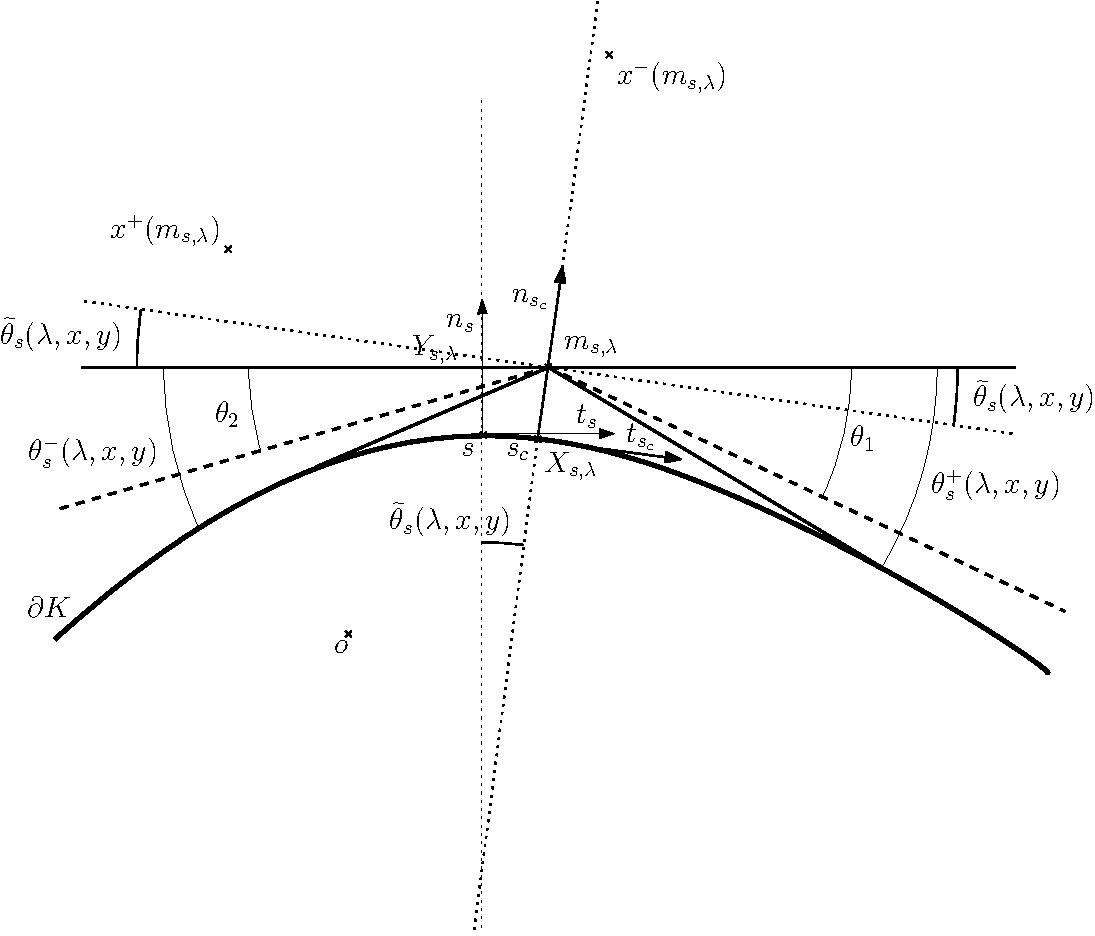
\includegraphics[scale=0.75]{supportsmooth.pdf}
\vspace{-0.2cm}
\caption{\label{fig:supportsmooth}
Realisation of the support function: $m_{s,\lambda}$ denotes the support point in the direction $n_s$.}
\end{center}
\end{figure}

%\noi
From a given $m_{s,\lambda}$ emanate two segments, one on the left of the half-line $\R_+m_{s,\lambda}$, one on the right. The symmetric points of $o$ with respect to these two segments define the right and the left Poisson--Voronoi neighbors of $o$ with respect to $m_{s,\lambda}$. They will be denoted by $x^+(m_{s,\lambda})$ and $x^-(m_{s,\lambda})$ respectively. Consequently, by Mecke--Slivnyak's formula, for every positive and measurable function $\varphi:\R^2\longrightarrow \R_+$,
\begin{multline*}\label{eq:convloi}
\E\left(\varphi\left(\lambda^{\frac1{3}}X_{s,\lambda},\lambda^{\frac{2}{3}}Y_{s,\lambda}\right)\right) \\
\begin{aligned}
& = \E\left(\sum_{(x_1,x_2)\,\in\,(\cP_{\lambda}\setminus2\cF_o(K))^2} {\emph{\indicat}}_{\left\{\substack{\scriptscriptstyle c_{x_1,x_2}\,=\,m_{s,\lambda}\\
x_1\,=\,x^+(m_{s,\lambda})\\x_2\,=\,x^-(m{s,\lambda})}\right\}}
\varphi\left(\lambda^{\frac1{3}}\langle c_{x_1,x_2}-s,t_s\rangle,\lambda^{\frac{2}{3}}\langle c_{x_1,x_2}-s,n_s\rangle\right)\right) \\
& = \lambda^2\int_{\R^2\times\R^2}\exp\left(-4\lambda\cA\left(B_{\frac{\|c_{x_1,x_2}\|}{2}}\left(\frac{c_{x_1,x_2}}{2}\right)\setminus\cF_o(K)\right)\right) {\emph{\indicat}}_{\left\{
\substack{\scriptscriptstyle{c_{x_1,x_2}\text{ is extreme in direction }n_s}\\
\scriptscriptstyle{x_1\,=\,x^+\left(c_{x_1,x_2}\right),\, x_2\,=\,x^-\left(c_{x_1,x_2}\right)}}
\right\}}
\end{aligned}\\
\times\varphi\left(\lambda^{\frac{1}{3}}\langle c_{x_1,\,x_2}-s,t_s\rangle,\lambda^{\frac{2}{3}}\langle c_{x_1,x_2}-s,n_s\rangle\right)\dd x_1 \dd x_2.
\end{multline*}

%\pass
We now apply two consecutive changes of variables in the integral above.

%\pass
First, we write $c_{x_1,x_2}= ru_{\theta}$ and denote by $\theta_1$ and $\theta_2$ the angles between one of the two bisecting lines emanating from $c_{x_1,x_2}$ and $t_{s}$. We then use Lemma~\ref{lem:jacob} to compute the corresponding Jacobian.

%\pass
Secondly, we replace the couple $(r,\theta)$ by $(x,y)$ defined by
\begin{equation*}\label{eq:xyh}
x=\lambda^{\frac1{3}}\langle c_{x_1,x_2}-s,t_s\rangle\,\text{ and }\, y=\lambda^{\frac{2}{3}}\langle c_{x_1,x_2}-s,n_s\rangle.
\end{equation*}

%\noi
We get in particular
\begin{equation}\label{eq:defrho}
\begin{cases}
r &=  \rho_s(\lambda,x,y)=\left(\left(\langle s,t_s\rangle+\lambda^{-\frac{1}{3}}x\right)^2+\left(\langle s,n_s\rangle+\lambda^{-\frac{2}{3}}y\right)^2\right)^\frac12 \\
\theta &=  \theta_s(\lambda,x,y) = \arccos\left(\left\langle \frac{s+\lambda^{-\frac1{3}}xt_s+\lambda^{-\frac{2}{3}}yn_s}{\bigl\|s+\lambda^{-\frac{1}{3}}xt_s+\lambda^{-\frac{2}{3}}yn_s\bigr\|},t_{s}\right\rangle\right)
\end{cases}
\end{equation}
where $\rho_s$ and $\theta_s$ are two functions of $\lambda$, $x$ and $y$, and a Jacobian given by
\[
\frac{r\dd r\dd \theta}{\dd x \dd y} = \lambda^{-1}.
\]
Consequently, we deduce that
\begin{multline}\label{eq:formuleexacte}
\E\left(\varphi\left(\lambda^{\frac1{3}}X_{s,\lambda},\lambda^{\frac{2}{3}}Y_{s,\lambda}\right)\right)\\
= 16\int_{\R\times \R_+}\exp\left(-\Delta_s(\lambda,x,y)\right)\varphi(x,y)\rho_s^2(\lambda,x,y)J^{\supp}_s(\lambda,x,y)\dd x \dd y
\end{multline}
where
\begin{align*}
\Delta_s(\lambda,x,y)&=4\lambda\cA\left(B_{\frac{\rho_s}{2}}\left(\frac{\rho_s u_{\theta_s}}{2}\right)\setminus \cF_o(K)\right)
\\
\intertext{and}
J^{\supp}_s(\lambda,x,y)&=\lambda\int_{E^{\supp}_{s,x,y}} J(\theta_s(\lambda,x,y),\theta_1,\theta_2)\dd \theta_1\dd \theta_2
\end{align*}
where $E^{\supp}_{s,x,y}$ stands for the set of couples $(\theta_1,\theta_2)$ which satisfy that $c_{x_1,x_2}$ is extremal in the direction of $n_s$ and that the two bisecting lines of $[o,x_1]$ and $[o,x_2]$ do not intersect $K$.

%\pass
Let us make the set $E^{\supp}_{s,x,y}$ explicit. Let $s_c$ be the orthogonal projection of $c_{x_1,x_2}$ onto $K$ and $t_{s_c}$ be the unit outer normal vector of $\partial K$ at $s_c$. We introduce the angles $\theta_s^+(\lambda,x,y)$, $\theta_s^-(\lambda,x,y)$ and $\widetilde{\theta}_s(\lambda,x,y)$ as, respectively, the angle of aperture at the point $c_{x_1,x_2}=s+\lambda^{-\frac1{3}}x t_s+\lambda^{-\frac{2}{3}}y n_s$ on the right, the angle of aperture at $c_{x_1,x_2}$ on the left and the angle between the vectors $n_s$ and $n_{s_c}$ (see Figure~\ref{fig:supportsmooth}). We obtain
\begin{multline}\label{eq:condanglessmooth}
(\theta_1,\theta_2)\in E^{\supp}_{s,x,y}\Longleftrightarrow -\theta_s^+(\lambda,x,y)-\widetilde{\theta}_s(\lambda,x,y)\\
< \theta_1<0<\theta_2<\theta_s^-(\lambda,x,y)-\widetilde{\theta}_s(\lambda,x,y).
\end{multline}

%\noi
In order to show the required convergence in distribution, we are going to use Lebesgue's dominated convergence theorem. To do so, we need to prove the convergence of the integrand in~\eqref{eq:formuleexacte} and that it is dominated.

%\pass
$-$ \emph{Convergence and domination of} $\rho_s(\lambda,x,y)$.

%\noi
We deduce from~\eqref{eq:defrho} that
\begin{equation}\label{eq:convrho}
\rho_s(\lambda,x,y)\underset{\lambda\to\infty}{\longrightarrow}\|s\|.
\end{equation}

%\noi
Moreover, by triangular inequality, we get for all $\lambda\ge 1$,
\begin{equation}\label{eq:dominationrho}
\rho_s(\lambda,x,y)\le \|s\|+\left(\lambda^{-\frac{2}{3}}x^2+\lambda^{-\frac{4}{3}}y^2\right)^{\frac1{2}}\le \|s\|+\|(x,y)\|.
\end{equation}

%\pass
$-$ \emph{Convergence and domination of} $\exp(-\Delta_s(\lambda,x,y))$.

%\noi
We denote by $h$ the distance from $c_{x_1,x_2}=s+\lambda^{-\frac1{3}}x t_s+\lambda^{-\frac{2}{3}}y n_s$ to $K$. Then the following relation holds, uniformly in $s$,
\begin{equation}\label{eq:hauteurdevue}
h\underset{\lambda\to\infty}{=}\lambda^{-\frac{2}{3}}\left(\frac{x^2}{2r_s}+y\right)+\Odd\left(\lambda^{-\frac{4}{3}}\right).
\end{equation}

%\noi
Moreover, there exists $C>0$ such that for every $s\in \partial K$ and all $\lambda\ge 1 $,
\begin{equation}\label{eq:dominationh}
C^{-1}\min\left(\lambda^{-\frac1{3}}\left(x^2+2yr_s\right)^{\frac1{2}},\lambda^{-\frac{2}{3}}\left(\frac{x^2}{r_s}+2y\right)\right)\le h\le C \lambda^{-\frac{2}{3}}\left(\frac{x^2}{2r_s}+y+\frac{y^2}{2r_s}\right).
\end{equation}

%\noi
Indeed, let us prove first~\eqref{eq:hauteurdevue} and~\eqref{eq:dominationh} when $K$ is a disk of radius $r_s$. We find on the one hand by Pythagoras' theorem
\[
\left\|c_{x_1,x_2}\right\|^2-r_s^2=\left(r_s+\lambda^{-\frac{2}{3}}y\right)^2+\lambda^{-\frac{2}{3}}x^2-r_s^2=\lambda^{-\frac{2}{3}}\left(x^2+\lambda^{-\frac{2}{3}}y^2+2r_sy\right)
\]
and on the other hand
\[
\|c_{x_1,x_2}\|^2-r_s^2=(\|c_{x_1,x_2}\|-r_s)(\|c_{x_1,x_2}\|+r_s)=h(2r_s+h).
\]
Combining these two equalities, we get
\[
h=r_s\left(1+\lambda^{-\frac{2}{3}}\left(\frac{x^2}{r_s^2}+\frac{2y}{r_s}+\lambda^{-\frac{2}{3}}\frac{y^2}{r_s^2}\right)\right)^{\frac1{2}}-r_s.
\]

%\noi
Using the estimate $\tfrac1{4}\min(u,u^{\frac1{2}})\le (1+u)^{\frac1{2}}-1\le\tfrac{u}{2}$ for every $u>0$ we obtain that the previous equality implies both~\eqref{eq:hauteurdevue} and~\eqref{eq:dominationh} when $K$ is a disk.

%\pass
When $K$ is a smooth convex body, we sandwich its boundary between two disks of radii $r_s+C'\lambda^{-\frac{2}{3}}$ and $r_s-C'\lambda^{-\frac{2}{3}}$ for a fixed positive constant $C'>0$ and we deduce from the previous case both~\eqref{eq:hauteurdevue} and~\eqref{eq:dominationh} for $K$.

%\noi
Moreover, using the regularity assumptions on the boundary $\partial K$, we get, uniformly in $s$,
\begin{equation}\label{eq:petitdetailtechnique}
\left|\langle s_c,n_{s_c}\rangle- \langle s,n_s\rangle\right|\underset{\lambda\to\infty}{=} \Odd\left(\lambda^{-\frac1{3}}\right).
\end{equation}

%\noi
Thanks to Lemma~\ref{lem:geom}, \eqref{eq:hauteurdevue} and~\eqref{eq:petitdetailtechnique}, we get, uniformly in $s$,
\begin{align}\label{eq:limiteaciter}
\Delta_s(\lambda,x,y) \underset{\lambda\to\infty}{\sim} 2^{\frac{9}{2}}3^{-1}r_{s}^{-\frac1{2}}\langle s,n_s\rangle\left(\frac{x^2}{2r_{s}}+y\right)^{\frac{3}{2}}.
\end{align}

%\noi
In particular, thanks to Lemma~\ref{lem:geom}$\MK$\eqref{eq:minorantvol} and~\eqref{eq:dominationh}, there exists $C>0$, uniform in~$s$, such that $\Delta_s(x,y)$ satisfies, for all $\lambda\ge 1$:
\begin{equation}\label{eq:dominationDelta}
\Delta_s(\lambda,x,y)\ge C \min\left(\left(x^2+2r_sy\right)^{\frac{3}{4}},\left(\frac{x^2}{2r_s}+y\right)^{\frac{3}{2}}\right).
\end{equation}\\

%\pass
$-$ \emph{Convergence and domination of} $J^{\supp}_s(\lambda,\,x,\,y)$.

%\noi
We start by estimating the function $\theta_s(\lambda,x,y)$. We get
\begin{equation}\label{eq:estimthetaxy}
\theta_s(\lambda,x,y)\underset{\lambda\to\infty}{=}\arcsin\left(\left\langle \frac{s}{\|s\|},n_s\right\rangle\right)+\Odd\left(\lambda^{-\frac1{3}}\right).
\end{equation}

%\noi
We now estimate the three angles $\theta_s^+(\lambda,x,y)$, $\theta_s^-(\lambda,x,y)$ and $\widetilde{\theta}_s(\lambda,x,y)$. Using~\eqref{eq:angleaperture} and~\eqref{eq:hauteurdevue}, we get
\begin{equation}\label{eq:estimtheta+}
\theta_s^+(\lambda,x,y) \underset{\lambda\to\infty}{=}\theta_s^-(\lambda,x,y)+\od\left(\lambda^{-\frac13}\right)
\underset{\lambda\to\infty}{=}\lambda^{-\frac1{3}} 2^{\frac1{2}}r_s^{-\frac1{2}}\left(\frac{x^2}{2r_s}+y\right)^{\frac1{2}}+ \od\left(\lambda^{-\frac13}\right).
\end{equation}

%\noi
Thanks to~\eqref{eq:dominationangleouverture} and~\eqref{eq:dominationh}, we have additionally the inequality, for some $C>0$,
\begin{equation}\label{eq:dominationtheta+}
\theta_s^+(\lambda,x,y)\le 2^{\frac1{2}}r_s^{-\frac1{2}}h^{\frac1{2}}\le C r_s\lambda^{-\frac1{3}}\left(\frac{x^2}{2r_s}+y+\frac{y^2}{2r_s}\right)^{\frac1{2}}.
\end{equation}

%\noi
The same inequality holds for $\theta_s^+(\lambda,x,y)$. We turn now our attention to $\widetilde{\theta}_s(\lambda,x,y)$. When $K$ is a disk we get
\[
\widetilde{\theta}_s(\lambda,x,y)=\arctan\left(\frac{\lambda^{-\frac1{3}}x}{r_s+\lambda^{-\frac{2}{3}}y}\right)
\underset{\lambda\to\infty}{=}\lambda^{-\frac1{3}}r_s^{-1}x+ \od\left(\lambda^{-\frac13}\right).
\]
%\noi
When $K$ is a smooth convex body, we sandwich again its boundary between two disks of radii $r_s+C\lambda^{-\frac{2}{3}}$ and $r_s-C\lambda^{-\frac{2}{3}}$ and we obtain
\begin{equation*}\label{eq:estimtildetheta}
\widetilde{\theta}_s(\lambda,x,y)\underset{\lambda\to\infty}{=}\lambda^{-\frac1{3}}r_s^{-1}x+\od\left(\lambda^{-\frac13}\right).
\end{equation*}

%\noi
Consequently, we deduce from~\eqref{eq:estimthetaxy}, \eqref{eq:condanglessmooth} and~\eqref{eq:estimtheta+} that
\begin{align}
&J^{\supp}_{s}(\lambda,x,y)\nonumber\\
& \underset{\lambda\to\infty}{\sim} \lambda\int_{E^{\supp}_{s,x,y}}\left|\sin(\theta_2-\theta_1)\sin(\theta_s(\lambda,x,y)-\theta_2)\sin(\theta_s(\lambda,x,y)-\theta_1)\right|
\dd \theta_1\dd \theta_2\nonumber \\
& \underset{\lambda\to\infty}{\sim}\lambda\sin^2\left(\arcsin\left(\left\langle\frac{s}{\|s\|},n_s\right\rangle\right)\right)\nonumber\\
&\mkern150mu \cdot \int_{\theta_1=-\theta_s^+(\lambda,x,y)\,-\widetilde{\theta}_s(\lambda,x,y)}^{0}
\int_{\theta_2=0}^{\theta_s^-(\lambda,x,y)\,-\widetilde{\theta}_s(\lambda,x,y)} (\theta_2-\theta_1)\dd \theta_1 \dd\theta_2\nonumber\\
& \underset{\lambda\to\infty}{\sim} \lambda \left\langle \frac{s}{\|s\|},n_s\right\rangle^2 \theta_s^+(\lambda,x,y)\left(\theta_s^+(\lambda,x,y)^2-\widetilde{\theta}_s(\lambda,x,y)^2\right)\nonumber\\
& \underset{\lambda\to\infty}{\sim} \left\langle \frac{s}{\|s\|},n_s\right\rangle^2 2^{\frac{3}{2}}r_s^{-\frac{3}{2}}y\left(\frac{x^2}{2r_s}+y\right)^{\frac1{2}}\label{eq:intangles}.
\end{align}


%\noi
Moreover, thanks to~\eqref{eq:dominationtheta+}, we get for some $C>0$,
\begin{equation}\label{eq:dominationJbarre}
J^{\supp}_{s}(\lambda,x,y)\le C r_s^3\left(\frac{x^2}{2r_s}+y+\frac{y^2}{2r_s}\right)^{\frac{3}{2}}.
\end{equation}\\
%\pass
$-$ \emph{Conclusion}.

%\noi
Combining~\eqref{eq:convrho}, \eqref{eq:limiteaciter} and~\eqref{eq:intangles}, we obtain that the integrand in~\eqref{eq:formuleexacte} converges to
\begin{equation*}
8\|s\|^2\varphi(x,y)\exp\!\left(-2^{-\frac{9}{2}}3^{-1}r_{s}^{-\frac1{2}}\left\langle s,n_s\right\rangle\left(\frac{x^2}{2r_{s}}+y\right)^{\frac{3}{2}} \right)\left\langle\frac{s}{\|s\|},n_s\!\right\rangle^2 2^{\frac{3}{2}}r_s^{-\frac{3}{2}}y\left(\frac{x^2}{2r_s}+y\!\right)^{\frac1{2}}.
\end{equation*}

%\noi
Now the estimates~\eqref{eq:dominationrho}, \eqref{eq:dominationDelta} and~\eqref{eq:dominationJbarre} show that we can apply Lebesgue's dominated convergence theorem for any function $\varphi$ bounded by a polynomial of $x$ and $y$, say. This proves assertion~\eqref{eq:ftheta} of Proposition~\ref{prop:supportsmooth}.
\end{prooff}

\begin{lastprooff}[{Proof of~\eqref{eq:convmean}}]
We start by rewriting~\eqref{eq:formuleexacte} when $\varphi(x,y)=y$:
\begin{equation}\label{eq:formuleYexacte}
\lambda^{\frac{2}{3}}\E(Y_{s,\lambda}) = 16\lambda^{\frac23}\int_{\R\times \R_+}\exp(-\Delta_s(\lambda,x,y))\rho_s^2(\lambda,x,y)J^{\supp}_s(\lambda,x,y)y\dd x \dd y.
\end{equation}
Thanks to~\eqref{eq:ftheta} applied to $\varphi(x,y)=y$, we can apply Lebesgue's dominated convergence theorem to get that
\begin{equation*}\label{eq:premiereformule}
\lambda^{\frac{2}{3}}\E(Y_{s,\,\lambda}) \underset{\lambda\to\infty}{\longrightarrow} 2^{\frac{11}{2}} r_s^{-\frac{3}{2}}\langle s,n_s\rangle^2I_s
\end{equation*}
where
\begin{equation*}\label{eq:defIs}
I_s =\int_{\R\times\R_+}\exp\left(-2^{\frac{9}{2}} 3^{-1}r_s^{-\frac1{2}}\left\langle s,n_s\right\rangle \left(\frac{x^2}{2r_s}+y\right)^{\frac{3}{2}}\right)\left(\frac{x^2}{2r_s}+y\right)^{\frac1{2}}y^2 \dd x \dd y.
\end{equation*}

%\noi
It remains to make the integral $I_s$ explicit. Recalling that $C_s= 2^{\frac{9}{2}}3^{-1}r_s^{-\frac1{2}}\,\langle s,n_s\rangle$, we get
\begin{equation*}\label{eq:decompIs}
I_s = \frac{4}{3 C_s}\int_0^{\infty}\left(\int_0^{\infty} e^{-u}\left(\frac{u^{\frac{2}{3}}}{C_s^{\frac{2}{3}}}-\frac{x^2}{2r_s}\right)^2 {\emph{\indicat}}_{\left\{0\,<\,x\,<\,2^{\frac1{2}}r_s^{\frac1{2}}C_s^{-\frac1{3}}u^{\frac1{3}}\right\}}\dd x\right)\dd u =I_s^{(1)}+I_s^{(2)}-I_s^{(3)}
\end{equation*}
where
\begin{align*}
I_s^{(1)} & = \frac{4}{3C_s}\int_0^{\infty}e^{-u}C_s^{-\frac{4}{3}}u^{\frac{4}{3}}2^{\frac1{2}}r_s^{\frac1{2}}C_s^{-\frac1{3}}u^{\frac1{3}}\dd u = 2^{\frac{5}{2}}3^{-2}5C_s^{-\frac{8}{3}}r_s^{\frac{1}{2}}\Gamma\left(\frac{5}{3}\right), \\
I_s^{(2)} & = \frac{4}{3C_s}\int_0^{\infty}e^{-u}20^{-1}r_s^{-2}\left(2^{\frac1{2}}r_s^{\frac1{2}}C_s^{-\frac1{3}}u^{\frac1{3}}\right)^5\dd u = 2^{\frac{5}{2}}3^{-2}C_s^{-\frac{8}{3}}r_s^{\frac{1}{2}}\Gamma\left(\frac{5}{3}\right),
\\
\intertext{and}
I_s^{(3)} &= \frac{4}{3C_s}\int_0^{\infty}e^{-u}C_s^{-\frac{2}{3}}r_s^{-1}3^{-1} u^{\frac{2}{3}}\left(2^{\frac1{2}}r_s^{\frac1{2}} C_s^{-\frac1{3}}u^{\frac1{3}}\right)^3\dd u = 2^{\frac{7}{2}}3^{-3}5C_s^{-\frac{8}{3}}r_s^{\frac{1}{2}}\Gamma\left(\frac{5}{3}\right).
\end{align*}

%\noi
Finally, inserting these equalities into $I_s$ yields the required result.
\end{lastprooff}\let\qed\relax
\end{proof}
%%$\square$
\vspace{0.2em}
\begin{proof}[{Proof of Theorem~\ref{theosmooth}$\MK$\eqref{theo1.1.ii}}]
We go back to the exact formula~\eqref{eq:formuleYexacte}. Since $K$ is a compact convex set with bounded positive curvature and containing the origin in its interior, the non-negative quantities $\|s\|$ and $r_s$ are bounded from above and from below. Consequently, the estimates~\eqref{eq:dominationrho}, \eqref{eq:dominationDelta} and~\eqref{eq:dominationJbarre} imply that the integral on the right-hand side of~\eqref{eq:formuleYexacte} is bounded independently of $s$, i.e. that there exists $C>0$ such that $\lambda^{\frac{2}{3}}\E(Y_{s,\lambda})\le C $ for every $s\in\partial K$.

%\noi
Consequently, we use Proposition~\ref{prop:supportsmooth}$\MK$\eqref{eq:convmean} and Lebesgue's dominated convergence theorem to get that
\begin{equation*}\label{eq:termedominantnbsommetssmooth}
\int_{\partial K} \E(Y_{s,\lambda})r_s^{-1} \dd s\underset{\lambda\to\infty}{\sim}\lambda^{-\frac{2}{3}} 3^{-\frac{4}{3}}\Gamma\left(\frac{2}{3}\right)\int_{\partial K} r_s^{-\frac{2}{3}}\langle s,n_s\rangle^{-\frac{2}{3}}\dd s.
\end{equation*}
The proof is completed thanks to Corollary~\ref{coro:appliEfronsmooth}$\MK$\eqref{coro2.2.1}.
\end{proof}
%$\square$


\subsection{Proof of Theorem~\ref{theosmooth}$\MK$\eqref{theo1.1.iii}: intensity and number of vertices}\label{subsec:verticessmooth}

\begin{proof}[{Proof of Theorem~\ref{theosmooth}$\MK$\eqref{theo1.1.iii}}]
Again, thanks to the convergence from Proposition~\ref{prop:supportsmooth}$\MK$\eqref{eq:convmean} and Lebesgue's dominated convergence theorem, we obtain that
\[
4\lambda\int_{\partial K}\langle s,n_s\rangle\E(Y_{s,\lambda})r_s^{-1}\dd s\underset{\lambda\to\infty}{\sim}\lambda^{\frac{1}{3}}2^2 3^{-\frac{4}{3}}\Gamma\left(\frac{2}{3}\right)\int_{\partial K} r_s^{-\frac{2}{3}}\left\langle s,n_s\right\rangle^{\frac1{3}}\dd s.
\]
Looking at Corollary~\ref{coro:appliEfronsmooth}$\MK$\eqref{coro2-2.2}, we observe that it is enough to show that
\begin{equation}\label{eq:restesmoothnegligible}
\lim_{\lambda\to\infty}\lambda^{-\frac13}{{\cR}_\lambda}=\lim_{\lambda\to\infty}2\lambda^{\frac23}\int_{\partial K}\E\left(Y_{s,\lambda}^2\right)r_s^{-1}\dd s=0.
\end{equation}
Applying~\eqref{eq:formuleexacte} to $\varphi(x,y)=y^2$ and using the estimates~\eqref{eq:dominationrho}, \eqref{eq:dominationDelta} and~\eqref{eq:dominationJbarre}, we get that there exists $C>0$ such that $\lambda^{\frac{4}{3}}\E(Y_{s,\lambda}^2)\le C $ for every $s\in\partial K$. This implies~\eqref{eq:restesmoothnegligible} and completes the proof of Theorem~\ref{theosmooth}$\MK$\eqref{theo1.1.iii}.
\end{proof}

%\pass
Actually, we can provide a more precise result on the asymptotic intensity of the point process of vertices of $K_{\lambda}^o$. This new result that we describe below could alternatively be used to get Theorem~\ref{theosmooth}$\MK$\eqref{theo1.1.iii} via an integration of the intensity given in the next proposition.

\begin{prop}\label{prop:intensitysmooth}
Let $s\in\partial K$ and consider the point process $(x_v,y_v)$ of the Cartesian coordinates of the vertices $v\in V_\lambda$ of $K_{\lambda}^o$ in the Cartesian orthonormal frame $(s,t_s,n_s)$. Let $A$ be a bounded Borel set of $\R^2\setminus K$ and denote by $\cN_s(A)$ the number of points of the rescaled point process
\[
\left(\lambda^{\frac1{3}}x_v,\lambda^{\frac{2}{3}}y_v\right)_{v\,\in\,V_\lambda}
\]
belonging to the set $A$. Then
\[
\E(\cN_s(A)) \underset{\lambda\to\infty}{\longrightarrow} \int_{A} \sigma_s(x,y)\dd x \dd y
\]
where
\begin{equation*}\label{eq:intensitysmooth}
\sigma_s(x,y)=2^{\frac{15}{2}}3^{-1}\exp\left(-2^{\frac{9}{2}}3^{-1} \left(\frac{x^2}{2r_s}+y\right)^{\frac{3}{2}} r_{s}^{-\frac1{2}}\langle s,n_s\rangle\right)
\langle s,n_s\rangle^2r_s^{-\frac{3}{2}}\left(\frac{x^2}{2r_s}+y\right)^{\frac{3}{2}}.
\end{equation*}
\end{prop}

\begin{proof}[{{Proof of Proposition~\ref{prop:intensitysmooth}}}]
The strategy is very similar to the proof of Proposition~\ref{prop:supportsmooth}, i.e. it consists in applying Mecke--Slivnyak's formula, then the change of variables provided by Lemma~\ref{lem:jacob} and finally Lebesgue's dominated convergence theorem.

%\pass
Consequently, we deduce that
\begin{align}\label{eq:calculintermcotes1}
\E(\cN_s(A)) = 16\int_{A}\exp(-\Delta_s(\lambda,x,y))\rho_s^2(\lambda,x,y)J^{\Vertt}_s(\lambda,x,y)\dd x \dd y
\end{align}
where
\begin{equation*}
J^{\Vertt}_s(\lambda,x,y) =\lambda\int_{E^{\Vertt}_{s,x,y}} J(\theta_s(\lambda,x,y),\theta_1,\theta_2)\dd \theta_1\dd \theta_2
\end{equation*}
and $E^{\Vertt}_{s,\,x,\,y}$ is the set of couples $(\theta_1,\theta_2)$ which satisfy that the two bisecting lines of $[o,x_1]$ and $[o,x_2]$ do not intersect $K$.

%\pass
Let us make the set $E^{\Vertt}_{s,x,y}$ explicit:
\begin{equation}\label{eq:condangles}
(\theta_1,\theta_2)\in E^{\Vertt}_{s,x,y}\Longleftrightarrow -\theta_s^+(\lambda,x,y)< \theta_1<\theta_2<\theta_s^-(\lambda,x,y).
\end{equation}


%\pass
The convergence and domination of $\rho_s(\lambda,x,y)$, $\exp(-\Delta_s(\lambda,x,y))$, $\theta_s^+(\lambda,x,y)$ and $\theta_s^-(\lambda,x,y)$ is identical to what has been done in the proof of Proposition~\ref{prop:supportsmooth}. We turn our attention to the convergence of $J^{\Vertt}_s(\lambda,x,y)$.
\begin{align}
&J^{\Vertt}_{s}(\lambda,x,y)\nonumber\\
& \underset{\lambda\to\infty}{\sim}\lambda \int_{E^{\Vertt}_{s,x,y}}\left|\sin(\theta_1-\theta_2)\sin(\theta_s(\lambda,x,y)-\theta_2)\sin\left(\theta_s(\lambda,x,y)-\theta_1\right)\right|
\dd \theta_1\dd \theta_2\nonumber\\
& \underset{\lambda\to\infty}{\sim} \lambda\sin^2\left(\arcsin\left(\left\langle \frac{s}{\|s\|},n_s\right\rangle\right)\right) \int_{\theta_1\,=\,-\theta_s^+(\lambda,\,x,\,y)}^{{\theta}_s^-(\lambda,\,x,\,y)}\int_{\theta_2=\theta_1}^{\theta_s^-(\lambda,x,y)}(\theta_2-\theta_1) \dd \theta_2 \dd\theta_1\nonumber\\
& \underset{\lambda\to\infty}{\sim} \frac{4}{3}\lambda \left\langle \frac{s}{\|s\|},n_s\right\rangle^2 \theta_s^+(\lambda,x,y)^3\nonumber\\
& \underset{\lambda\to\infty}{\sim} 2^{\frac{7}{2}}3^{-1}\left\langle \frac{s}{\|s\|},n_s\right\rangle^2 r_s^{-\frac{3}{2}}\left(\frac{x^2}{2r_s}+y\right)^{\frac{3}{2}}.\label{eq:convJbarre2}
\end{align}

%\pass
Moreover, thanks to~\eqref{eq:dominationtheta+}, we get for some positive constant $C>0$,
\begin{equation}\label{eq:dominationJbarre2}
J^{\Vertt}_{s}(\lambda,x,y)\le C \left\langle \frac{s}{\|s\|},n_s\right\rangle^2r_s^{-\frac{3}{2}}\left(\frac{x^2}{2r_s}+y\right)^{\frac{3}{2}}.
\end{equation}

%\pass
Combining~\eqref{eq:convrho}, \eqref{eq:limiteaciter} and~\eqref{eq:convJbarre2}, we obtain that the integrand in~\eqref{eq:calculintermcotes1} converges to
\[
2^{\frac{15}{2}}3^{-1}\exp\left(-2^{\frac{9}{2}}3^{-1} \left(\frac{x^2}{2r_s}+y\right)^{\frac{3}{2}} r_{s}^{-\frac1{2}}\langle s,n_s\rangle\right)
\langle s,n_s\rangle^2r_s^{-\frac{3}{2}}\left(\frac{x^2}{2r_s}+y\right)^{\frac{3}{2}}.
\]

%\pass
Now the estimates~\eqref{eq:dominationrho}, \eqref{eq:dominationDelta} and~\eqref{eq:dominationJbarre2} show that we can apply Lebesgue's dominated convergence theorem. The result follows.
\end{proof}
%$\square$~\\

%\noi
Proposition~\ref{prop:intensitysmooth} provides an extra valuable information on the point process of vertices which is clearly not of Poisson type. To some extent, this is also reminiscent of the description of the rescaled point process of vertices of random polytopes in the unit-ball or random Gaussian polytopes, as a sub-product of a growth parabolic process based on a Poisson point process, see e.g.~\cite[Theorem~4.1]{CSY}. We skip the proof of Proposition~\ref{prop:intensitysmooth} as it is in the same spirit as the proof of Proposition~\ref{prop:supportsmooth}.



\section{The polygonal case}\label{sec:polygon}

%\noi
In this section $K$ is a convex polygon with vertices $a_1,a_2,\,\ldots,\,a_{n_K}$ containing the origin $o$ in its interior. We denote by $\alpha_i$ the interior angle at vertex $a_i$ and we recall that $o_i$ is the orthogonal projection of $o$ onto the line $(a_i,a_{i+1})$. A point outside $K$ will be located by its polar coordinates from one vertex $a_i$ (see Figure~\ref{fig:polygonsurf}), i.e. we consider a point $s_{a_i,\rho,\alpha}=a_i+\rho u_{\pi-\alpha}$ in the neighborhood of $a_i$, with $\rho>0$ and $\alpha\in(0,\alpha_i)$.

%\pass
The different proofs of the results of this Section will require to decompose the set $\R^2\setminus K$ into several regions, namely $n_K$ cones above the vertices of $K$ and $n_K$ strips above the edges of $K$. More precisely, for every $1\le i \le n_K$, let us define the cones
\begin{align*}
\cG_i &=\left\{s_{a_i,\rho,\alpha}:\rho>0 \text{ and } \alpha\in\left(\frac{\pi}{2},\frac{3\pi}{2}-\alpha_i\right)\right\}
\\
\intertext{and the strip}
\cS_i &=\left\{s_{a_i,\rho,\alpha}:\rho>0 \text{ and } \rho\cos\alpha\in(0,\|a_{i+1}-a_i\|)\right\}
\end{align*}
as the connected component of $\R^2\setminus (K\cup(\cup_{i=1}^{n_K}\cG_i))$ with $(a_i,a_{i+1})$ on its boundary.


\subsection{Increase of the area of the Voronoi flower}\label{subsec:fleurpoly}

%\pass

%\noi
First, the following geometric lemma provides accurate estimates of the area of the set
\begin{equation*}\label{def:diffvorflowpoly}
\Delta\cF_{a_i,\rho,\alpha}=\cF_o(K \cup \left\{s_{a_i,\rho,\alpha}\right\})\setminus\cF_o(K).
\end{equation*}

\begin{lemm}\label{lem:geompoly1}
Assume that $K$ is a convex polygon and let $a_i\in\partial K$, $1\leq i \leq n_K$, be a fixed vertex of $K$.
\begin{enumerate}\romanenumi
\item\label{estimeevolfleurpoly1} We get, uniformly in $\rho>0$,
\[
\cA(\Delta\cF_{a_i,\rho,\alpha})\indicat_{\left\{s_{a_i,\rho,\alpha}\,\in\,\cS_i\right\}}\underset{\alpha\,\to\,0}{\sim} \alpha^2\frac{\|o_i\|}{2}\frac{\rho\|a_{i+1}-a_i\|}{\|a_{i+1}-a_i\|-\rho}.
\]
\item\label{estimeevolfleurpoly2} Moreover, there exists $C>0$ such that, for all $(\rho,\alpha)$ such that $s_{a_i,\rho,\alpha}$ belongs to $\cG_i\cup\cS_i$,
\[
\cA\left(\Delta\cF_{a_i,\rho,\alpha}\right)\ge C\max(1,\rho)\rho\alpha^2.
\]
\end{enumerate}
\end{lemm}

\begin{proof}[{Proof of Lemma~\ref{lem:geompoly1}.}]

\begin{prooff}[{Proof of~\eqref{estimeevolfleurpoly1}}]
For $\alpha$ small enough, the set $\Delta \cF_{a_i,\rho,\alpha}$ is nothing but
\begin{equation*}\label{eq:fleurdecompdisques}
\Delta \cF_{a_i,\rho,\alpha}=B_{\frac1{2}\left\|s_{a_i,\rho,\alpha}\right\|}\left(\frac1{2} s_{a_i,\rho,\alpha}\right)\setminus \left(B_{\frac1{2}\|a_i\|}\left(\frac{1}{2}a_i\right)\cup B_{\frac{1}{2}\|a_{i+1}\|}\left(\frac1{2}a_{i+1}\right)\right),
\end{equation*}
that is a curvilinear triangle with vertices $o_i$, $a_i'$ and $a_{i+1}'$ where $a_i'$ and $a_{i+1}'$ are respectively the intersection of
\[
\partial B_{\frac1{2}\left\|s_{a_i,\rho,\alpha}\right\|}(\frac1{2} s_{a_i,\rho,\alpha})\text{ with }\partial B_{\frac1{2}\|a_i\|}\left(\frac1{2}a_i\right)\text{ and }\partial B_{\frac1{2}\|a_{i+1}\|}\left(\frac1{2}a_{i+1}\right)
\]
(see Figure~\ref{fig:polygonsurf}).

\begin{figure}[h!]
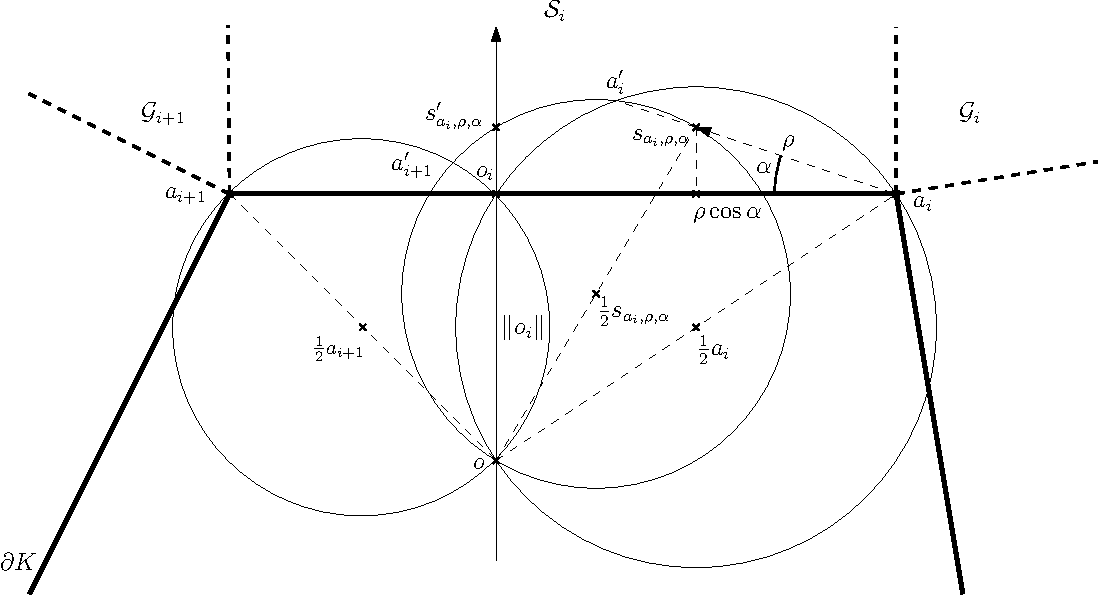
\includegraphics[scale=0.8]{polygonsurf.pdf}
\caption{\label{fig:polygonsurf}
The influence on the Voronoi flower of $K$ of adding an extra point $s_{a_i,\rho,\alpha}$ in a neighborhood of its boundary viewed from the origin $o$.}
\end{figure}

%\pass
We aim at computing estimates for the area $\cA(\Delta\cF_{a_i,\rho,\alpha})$ of this curvilinear triangle. To do this, we split it into the curvilinear triangles with vertices $o_i$, $s_{a_i,\rho,\alpha}'$, $a_i'$ and $o_i$, $s_{a_i,\rho,\alpha}'$, $a_{i+1}'$ respectively, where $s_{a_i,\rho,\alpha}'$ is the intersection of the line $(o,o_i)$ with the circle
\[
\partial B_{\frac1{2}\left\|s_{a_i,\rho,\alpha}\right\|}\left(\frac1{2} s_{a_i,\rho,\alpha}\right)\,.
\]

%\pass
Let us focus on the first curvilinear triangle. As $\alpha\to0$, it tends to a straight triangle whose area is given by
\[
\cA\left(o_i s_{a_i,\rho,\alpha}' a_i'\right)\underset{\alpha\to 0}{\sim} \frac1{2}\left\|s'_{a_i,\rho,\alpha}-o_i\right\|\left(\left\|\overset{\frown}{a_i'o_i}\right\|\sin\beta_i\right)
\]
where $\beta_i$ is the angle between the line $(o_i,s'_{a_i,\rho,\alpha})$ and the tangent line to the disk $B_{\tfrac{1}{2}a_i}(\tfrac{1}{2}\|a_i\|)$ at $o_i$.

%\pass
Observe first that we get by symmetry $\|s'_{a_i,\rho,\alpha}-o_i\| = \rho\sin \alpha$.

%\noi
Let us now compute the length of the arc $\overset{\frown}{a_i'o_i}$. Observe now that the lines $(s_{a_i,\rho,\alpha},a_i')$ and $(a_i,a_i')$ are both perpendicular to $(o,a_i')$. Therefore the points $a_i, s_{a_i,\rho,\alpha}$ and $a_i'$ are aligned. It follows that the angle between the lines $(a_i,a_{i+1})$ and $(a_i,a_i')$ is the same as the angle between $(a_i,a_{i+1})$ and $(a_i,s_{a_i,\rho,\alpha})$ which is nothing but $\alpha$. Thus the central angle between the lines $(\tfrac{1}{2}a_i,a_i')$ and $(\tfrac{1}{2}a_i,o_i)$ is $2\alpha$. Since the arc $\overset{\frown}{a_i'o_i}$ belongs to the circle with center $\tfrac{1}{2}a_i$ and diameter $\|a_i\|$ we get
\[
\|\overset{\frown}{a_i'o_i}\| = \frac1{2}\|a_i\|(2\alpha) = \|a_i\|\alpha.
\]

%\noi
Finally, observing that $\beta_i$ is equal to the angle between $(a_i,o_i)$ and $(a_i,o)$ by the inscribed angle theorem, we deduce that
\begin{align*}
\cA\left(o_i s_{a_i,\rho,\alpha}' a_i'\right) &\underset{\alpha\to 0}{\sim} \frac1{2}\left(\rho\sin \alpha\right)\left(\|a_i\|\alpha\sin\beta_i \right) \\
&= \frac1{2}\left(\rho\sin \alpha\right)\left(\|a_i\|\alpha \frac{\|o_i\|}{\|a_i\|}\right)
\underset{\alpha\to 0}{\sim} \frac1{2}\rho \alpha^2\|o_i\|.
\end{align*}

%\noi
Now, computing similarly the area $\cA(o_i s_{a_i,\rho,\alpha}' a_{i+1}')$ of the other curvilinear triangle, we obtain
\[
\cA\left(o_i s_{a_i,\rho,\alpha}' a_{i+1}'\right) = \frac1{2}\rho' \alpha'^2\|o_i\|
\]
where
\[
\begin{cases}
\rho' & = \Big((\|a_{i+1}-a_i\|-\rho\cos\alpha)^2+(\rho\sin\alpha)^2\Big)^{\frac1{2}} \underset{\alpha\to 0}{\sim} \|a_{i+1}-a_i\|-\rho \\
\alpha' & = \arctan\left(\frac{\rho\sin\alpha}{\|a_{i+1}-a_i\|-\rho\cos\alpha}\right) \mkern120mu\underset{\alpha\to 0}{\sim} \frac{\rho\alpha}{\|a_{i+1}-a_i\|-\rho}
\end{cases}
\]

%\noi
Therefore,
\[
\cA\left(o_i s_{a_i,\rho,\alpha}' a_{i+1}'\right) \underset{\alpha\to 0}{\sim} \frac1{2}\frac{\rho^2\alpha^2\|o_i\|}{\|a_{i+1}-a_i\|-\rho}\,.
\]

%\noi
Finally, summing the areas of each triangle, we obtain
\[
\cA\left(\Delta\cF_{a_i,\rho,\alpha}\right)\underset{\alpha\to0}{\sim} \frac1{2}\rho\alpha^2\|o_i\|\bigg(1+\frac{\rho}{\|a_{i+1}-a_i\|-\rho}\bigg)
\underset{\alpha\to0}{\sim} \frac1{2}\rho\alpha^2\|o_i\|\frac{\|a_{i+1}-a_i\|}{\|a_{i+1}-a_i\|-\rho}
\]
so that~\eqref{estimeevolfleurpoly1} holds.
\end{prooff}

\begin{lastprooff}[{Proof of~\eqref{estimeevolfleurpoly2}}]
We first assume that $s_{a_i,\rho,\alpha}\in \cS_i$. Because of point (i), there exists $\alpha_0\in (0,\tfrac{\pi}{2})$ such that for every $\alpha<\alpha_0$, $\cA(\Delta\cF_{a_i,\rho,\alpha})\ge \tfrac{\|o_i\|}{4}\rho\alpha^2$ and $\rho\le \tfrac{\|a_{i+1}-a_i\|}{\cos\alpha_0}$. This proves the result as soon as $\alpha<\alpha_0$. When $\alpha>\alpha_0$, it is enough to show that $ \cA(\Delta\cF_{a_i,\rho,\alpha})\ge C \max (\rho,\rho^2)$ for some positive constant $C$. This last inequality comes now from the fact that $\Delta\cF_{a_i,\rho,\alpha}$ contains both a disk of radius proportional to $\rho$ and an angular sector with thickness $\rho$ and constant angular width.~Finally, the exact same argument holds when $s_{a_i,\rho,\alpha}\in \cG_i$ so this completes the proof.
\end{lastprooff}\let\qed\relax
\end{proof}
%$\square$


\subsection{Proof of Theorem~\ref{theopolygon}$\MK$\eqref{theo1.2.i}: the defect area}\label{subsec:surfacepolygon}

%\pass

%\noi
\begin{proof}[{Proof of Theorem~\ref{theopolygon}$\MK$\eqref{theo1.2.i}}]
Recalling the notation of Section~\ref{subsec:fleurpoly} and using~\eqref{eq:airesmooth}, we can write $\E(\cA(K_{\lambda}^o)) -\cA(K)$ as
\begin{align*}
\sum_{i=1}^{n_K}\left(\int_{\cS_i}\exp\left(-4\lambda\cA\left(\Delta\cF_{a_i,\rho,\alpha}\right)\right)\rho\dd \rho \dd\alpha + \int_{\cG_i}\exp\left(-4\lambda\cA\left(\Delta\cF_{a_i,\rho,\alpha}\right)\right) \rho\dd \rho \dd \alpha \right).
\end{align*}

%\noi
It is then enough to show that, for every $1\le i\le n_K$,
\begin{equation}\label{eq:madonna}
\lambda^{\frac1{2}}\int_{\cS_i}\exp\left(-4\lambda\cA\left(\Delta\cF_{a_i,\rho,\alpha}\right)\right)\rho\dd \rho \dd\alpha
\underset{\lambda\to\infty}{\longrightarrow} 2^{-\frac{9}{2}}\pi^{\frac{3}{2}}\|o_i\|^{-\frac1{2}}\|a_{i+1}-a_i\|^{\frac{3}{2}}
\end{equation}
and
\begin{equation}\label{eq:rayoflight}
\lambda^{\frac{1}{2}}\int_{\cG_i}\exp\left(-4\lambda\cA\left(\Delta\cF_{a_i,\rho,\alpha}\right)\right) \rho\dd \rho \dd \alpha
\underset{\lambda\to\infty}{\longrightarrow} 0.
\end{equation}

%\noi
Let us prove~\eqref{eq:madonna} first. Let us fix $1\le i\le n_K$. The change of variables $\beta=\lambda^{\frac1{2}}\alpha$ yields
\begin{multline*}
\lambda^{\frac1{2}}\int_{\cS_i}\exp \left(-4\lambda \cA\left(\Delta\cF_{a_i,\rho,\alpha}\right)\right)\rho\dd \rho \dd\alpha\\
= \int_{0}^{\rho_i(\lambda^{-1/2}\beta)}\int_{0}^{\lambda^{1/2}\frac{\pi}{2}}
\exp\left(-4\lambda\cA\left(\Delta\cF_{a_i,\rho,\lambda^{-1/2}\beta}\right)\right)\rho\dd \rho \dd\beta
\end{multline*}
where $\rho_i(\cdot)$ denotes the equation of the line containing $a_{i+1}$ and orthogonal to $(a_{i},a_{i+1})$ with respect to the polar coordinates $(\rho,\alpha)$, i.e. $\rho_i(\alpha)$ is the distance from the origin to the intersection between that line and $\R_+ u_\alpha$.

%\noi
Thanks to Lemma~\ref{lem:geompoly1}, we have
\[
4\lambda\cA\left(\Delta\cF_{a_i,\rho,\lambda^{-1/2}\beta}\right) \underset{\lambda\to\infty}{\longrightarrow} 2\|o_i\|\frac{\rho\|a_{i+1}-a_i\|}{\|a_{i+1}-a_i\|-\rho}\beta^2
\]
and, for all $\lambda>0$,
\[
\lambda\cA\left(\Delta\cF_{a_i,\rho,\lambda^{-1/2}\beta}\right) \ge C \max(1,\rho)\rho \beta^2
\]
where $C$ is a positive constant.

%\noi
Consequently, we can apply Lebesgue's dominated convergence theorem to obtain
\begin{multline*}
\int_0^{\rho_i\left(\lambda^{-1/2}\beta\right)}\int_{0}^{\lambda^{1/2}\frac{\pi}{2}}
\exp\left(-4\lambda\cA\left(\Delta\cF_{a_i,\rho,\lambda^{-1/2}\beta}\right)\right)\rho\dd \rho \dd\beta \\
\begin{aligned}
& \underset{\lambda\to\infty}{\longrightarrow} \int_0^{\left\|a_{i+1}-a_i\right\|}\int_0^{\infty}
\exp\left(-2\|o_i\|\frac{\rho\|a_{i+1}-a_i\|}{\|a_{i+1}-a_i\|-\rho}\beta^2 \right)\rho\dd \rho \dd\beta \\
& = \left\|a_{i+1}-a_i\right\|^2\int_0^1\left(\int_0^{\infty} \exp\left(-2\|o_i\|\frac{l\|a_{i+1}-a_i\|}{1-l}\beta^2 \right)\dd\beta \right) l\dd l \\
& = \|a_{i+1}-a_i\|^{\frac{3}{2}} \pi^{\frac1{2}}2^{-\frac{3}{2}}\|o_i\|^{-\frac1{2}} \int_0^1 (l(1-l))^{\frac1{2}}\dd l \\
& = \|a_{i+1}-a_i\|^{\frac{3}{2}} \pi^{\frac{3}{2}}2^{-\frac{9}{2}}\|o_i\|^{-\frac1{2}}.
\end{aligned}
\end{multline*}

%\pass
Let us turn to the proof of~\eqref{eq:rayoflight}. Using the second part of Lemma~\ref{lem:geompoly1} we have successively, for all $\lambda>0$,
\begin{multline*}
\int_{\cG_i}\exp\left(-4\lambda\cA\left(\Delta\cF_{a_i,\rho,\alpha}\right)\right) \rho\dd \rho \dd \alpha \\
\begin{aligned}
& \leq \int_0^{\infty}\int_{\frac{\pi}{2}}^{\frac{3\pi}{2}-\alpha_i}\exp\left(-C\lambda\max(1,\rho)\rho\alpha^2\right) \rho\dd \rho \dd \alpha \\
& = \int_{\frac{\pi}{2}}^{\frac{3\pi}{2}-\alpha_i}\left(\int_0^1\exp\left(-C\lambda\rho\alpha^2\right) \rho\dd \rho\right) \dd \alpha + \int_{\frac{\pi}{2}}^{\frac{3\pi}{2}-\alpha_i}\left(\int_1^{\infty}\exp\left(-C\lambda\rho^2\alpha^2\right) \rho\dd \rho\right) \dd \alpha \\
& \leq \int_{\frac{\pi}{2}}^{\frac{3\pi}{2}-\alpha_i} \lambda^{-2}\alpha^{-4} \dd \alpha + \int_{\frac{\pi}{2}}^{\frac{3\pi}{2}-\alpha_i} \lambda^{-1}\alpha^{-2} \dd \alpha \\
& \leq C \lambda^{-1}.
\end{aligned}
\end{multline*}

%\noi
That implies~\eqref{eq:rayoflight} and completes the proof of Theorem~\ref{theopolygon}$\MK$\eqref{theo1.2.i}.
\end{proof}


\subsection{Proof of Theorem~\ref{theopolygon}$\MK$\eqref{theo1.1.ii}: support points and defect perimeter}\label{sub:perimeterpolygon}

%\pass

%\noi
As in the smooth case, the strategy consists in using Corollary~\ref{coro:appliEfronpolygonal} and estimating the defect support function
\[
Z_{i,\gamma,\lambda,-}= p_o\left(K_{\lambda}^o,\delta_i-\lambda^{-\gamma}\right)-p_o\left(K,\delta_i-\lambda^{-\gamma}\right)
\]
of $K_{\lambda}^o$ in a fixed direction $\delta_i-\lambda^{-\gamma}$, $1\le i\le n_K$. As emphasized in the proof of point~\eqref{theo1.1.ii} of Theorem~\ref{theopolygon}, we will treat separately the cases $\gamma\in(0,\tfrac1{2})$ and $\gamma\ge \tfrac1{2}$. More precisely, let us introduce the support point $m_{\lambda^{-\gamma}}$ on $\partial K_{\lambda}^o$ which satisfies
\[
\left\langle m_{\lambda^{-\gamma}}, u_{\delta_i-\lambda^{-\gamma}}\right\rangle=p_o\left(K_{\lambda}^o,\delta_i-\lambda^{-\gamma}\right)
\]
and let us denote by $(R_{\lambda^{-\gamma}},A_{\lambda^{-\gamma}})$ the polar coordinates of $m_{\lambda^{-\gamma}}$ with respect to the coordinate system with origin $a_i$ and first axis $(a_i,a_{i+1})$. In particular, we notice that $A_{\lambda^{-\gamma}}\ge \lambda^{-\gamma}$ almost surely since $p_o(K_{\lambda}^o,\delta_i-\lambda^{-\gamma})\ge p_o(K,\delta_i-\lambda^{-\gamma})\ge \langle a_i,u_{\delta_i-\lambda^{-\gamma}}\rangle$.

%\pass
The next Proposition investigates the asymptotic distribution of the couple $(R_{\lambda^{-\gamma}},\linebreak A_{\lambda^{-\gamma}})$ for $\gamma\in (0,\tfrac12)$.

\begin{prop}\label{prop:supportpoly}
%\noi
Let $a_i\in\partial K$, $1\leq i \leq n_K$, be a fixed vertex of $K$.
\begin{enumerate}\romanenumi
\item \label{eq:fthetapoly}For every $\gamma\in (0,\tfrac{1}{2})$, the couple $(\lambda^{1-2\gamma}R_{\lambda^{-\gamma}}, \lambda^{\gamma}A_{\lambda^{-\gamma}})$ converges in distribution when $\lambda\to\infty$ to the distribution with density function $f_i$ given by
\[
f_i(\rho,\alpha)= 8\|o_i\|^2\exp\left(-2\|o_i\|\rho\alpha^2\right)\alpha(\alpha-1)\rho \indicat_{\{\rho\,>\,0\}}\indicat_{\{\alpha\,>\,1\}}.
\]
\item \label{eq:estimsupppolyg} There exists $C>0$ such that for every $\gamma\in (0,\tfrac{1}{2})$ and $\lambda>0$,
\[
\lambda^{1-\gamma}\E\left(R_{\lambda^{-\gamma}}\sin\left(A_{\lambda^{-\gamma}}-\lambda^{-\gamma}\right)\right)\le C.
\]
\item \label{prop4.2.3}Moreover, for every $\gamma\in (0,\tfrac{1}{2})$,
\[
\E\left(Z_{i,\,\gamma,\,\lambda,-}\right) = \E\left(R_{\lambda^{-\gamma}}\sin\left(A_{\lambda^{-\gamma}}-\lambda^{-\gamma}\right)\right)
\underset{\lambda\to\infty}{\sim}\lambda^{\gamma-1}\frac1{6\|o_i\|}.
\]
\end{enumerate}
\end{prop}


\begin{proof}[{Proof of Proposition~\ref{prop:supportpoly}.}]
\begin{prooff}[{Proof of~\eqref{eq:fthetapoly}}]
Without loss of generality, we can assume in the proof that $\delta_i=\tfrac{\pi}{2}$. Once again, the strategy of the proof consists in going along the same lines as for the smooth case. We start with the same identity but written in polar coordinates, that is $c_{x_1,x_2}=m_{\lambda^{-\gamma}}= a_i+ru_{\theta}$ (see Figure~\ref{fig:supportpolygon}). Notice that $(r,\theta)\in\cS_i$ when $\lambda\to\infty$.

\begin{figure}[h!]
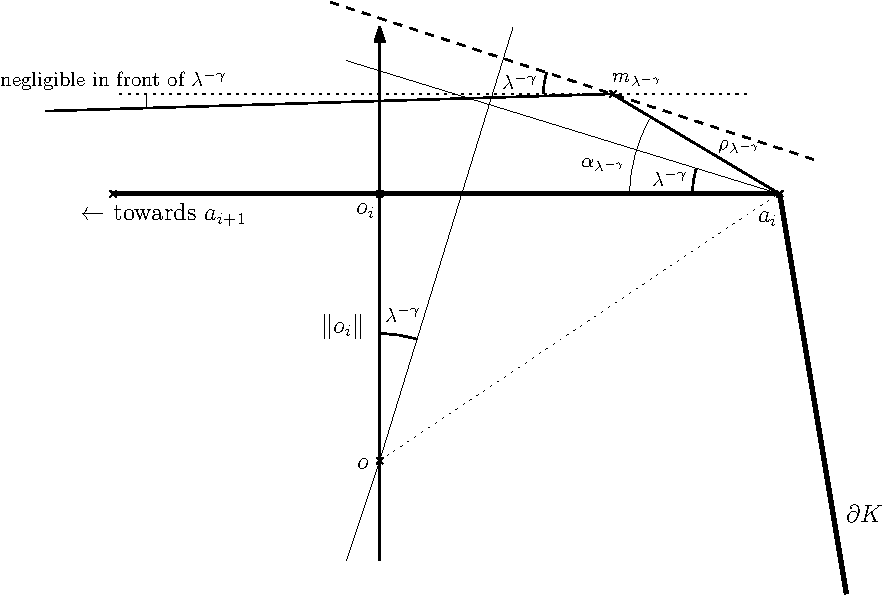
\includegraphics[scale=0.8]{supportpolygon.pdf}
\caption{\label{fig:supportpolygon}
The analogue of Figure~\ref{fig:supportsmooth} in the polygonal case: $m_{\lambda^{-\gamma}}$ denotes the support point in the direction $\tfrac{\pi}{2}-\lambda^{-\gamma}$.}
\end{figure}

%\pass
 We then proceed with two consecutive changes of variables. First, denoting by $\theta_1$ and $\theta_2$ the angles between the two bisecting lines emanating from $c_{x_1,x_2}$ corresponding to the right and left neighbor of $o$ respectively, we use Lemma~\ref{lem:jacob}. Secondly, we replace the couple $(r,\theta)$ by $(\rho,\alpha)$ defined by
\begin{align*}
\rho = \lambda^{1-2\gamma}r \,\text{ and }\, \alpha=\lambda^{\gamma}\theta.
\end{align*}

%\noi
We get in particular
\[
\begin{cases}
r & =  r_i(\lambda,\rho,\alpha)=\left\|s_{a_i,\lambda^{2\gamma-1}\rho,\lambda^{-\gamma}\alpha}\right\| \\
\theta & =  \theta_i(\lambda,\rho,\alpha) = \arcsin\left(\left\langle \frac{s_{a_i,\lambda^{2\gamma-1}\rho,\,\lambda^{-\gamma}\alpha}}{\bigl\|s_{a_i,\lambda^{2\gamma-1}\rho,\lambda^{-\gamma}\alpha}\bigr\|},\frac{o_i}{\|o_i\|}\right\rangle\right)
\end{cases}
\]
and a Jacobian given by $\tfrac{r\dd r \dd \theta }{\rho\dd\rho \dd\alpha} = \lambda^{3\gamma-2}$. Consequently, as in the proof of point~\eqref{eq:ftheta} of Proposition~\ref{prop:supportsmooth}, we deduce that for every positive and measurable function $\varphi:\R^2\longrightarrow \R_+$
\begin{multline*}
\E\left(\varphi\left(\lambda^{1-2\gamma}R_{\lambda^{-\gamma}}, \lambda^{\gamma}A_{\lambda^{-\gamma}}\right)\right) \\
= 16\int_1^{\lambda^{\gamma}\pi+1}\int_0^{\lambda^{1-2\gamma}\rho_i(\alpha)}\exp\left(-\Delta_i\left(\lambda,\rho,\alpha\right)\right)r_i^2(\lambda,\rho,\alpha) J^{\supp}_i(\lambda,\rho,\alpha)\varphi(\rho,\alpha)\rho\dd\alpha\dd \rho \\
\end{multline*}
where
\begin{multline*}
\Delta_i(\lambda,\rho,\alpha)\\
= 4\lambda\cA\left(B_{\left\|s_{a_i,\lambda^{2\gamma-1}\rho,\lambda^{-\gamma}\alpha}\right\|}\left(s_{a_i,\lambda^{2\gamma-1}\rho,\lambda^{-\gamma}\alpha}\right)\setminus \cF_o(K)\right) = 4\lambda\cA\left(\Delta \cF_{a_i,\lambda^{2\gamma-1}\rho,\lambda^{-\gamma}\alpha}\right)
\end{multline*}
and
\[
J^{\supp}_i(\lambda,\rho,\alpha)=\lambda^{3\gamma}\int_{E_i(\lambda,\rho,\alpha)} J\left(\theta_i(\lambda,\rho,\alpha),\theta_1,\theta_2\right)\dd \theta_1\dd \theta_2
\]
where $E_i^{\supp}(\lambda,\rho,\alpha)$ stands for the set of couples $(\theta_1,\theta_2)$ which satisfy that the two bisecting lines of $[o,x_1]$ and $[o,x_2]$ do not intersect $K$.

%\pass
Thanks to Lemma~\ref{lem:geompoly1}, we have
\begin{align*}
\Delta_i(\lambda,\rho,\alpha) \underset{\lambda\to\infty}{\longrightarrow} 2\|o_i\|\rho\alpha^2
\end{align*}
as soon as $\lambda^{2\gamma-1}\rho\cos(\lambda^{-\gamma}\alpha)\le \|a_{i+1}-a_i\|$ and
\begin{equation}\label{eq:dominDeltapolyg}
\Delta_i(\lambda,\rho,\alpha)\ge C \rho \alpha^2
\end{equation}
for some constant $C>0$. Moreover,
\begin{align*}
r_i(\lambda,\rho,\alpha) \underset{\lambda\to\infty}{\longrightarrow} \|a_i\|
\end{align*}
and for $\lambda\ge 1$,
\begin{equation}\label{eq:dominripolyg}
r_i(\lambda,\rho,\alpha)\le \|a_i\|+\lambda^{2\gamma-1}\rho\le \|a_i\|+\rho.
\end{equation}

%\pass
Let us now turn on the term $J^{\supp}_i(\lambda,\rho,\alpha)$. Using the convergence
\[
\sin(\theta_i(\lambda,\rho,\alpha))\underset{\lambda\to\infty}{\longrightarrow} \frac{\|o_i\|}{\|a_i\|},
\]
we get successively
\begin{multline*}
J^{\supp}_i(\lambda,\,\rho,\,\alpha) \\
\begin{aligned}
& \!\!\underset{\lambda\to\infty}{\sim} \lambda^{3\gamma}\int_{E_i(\lambda,\rho,\alpha)}J(\theta_i(\lambda,\rho,\alpha),\theta_1,\theta_2)\dd \theta_1\dd \theta_2 \\
&\!\! \underset{\lambda\to\infty}{\sim}\!\!\!\lambda^{3\gamma}\!\!\!\int_{\left(0,(\alpha-1)\lambda^{-\gamma}\right)\times(0,\lambda^{-\gamma})}\!\!\left|\sin(\theta_i(\lambda,\rho,\alpha)-\theta_1)\sin(\theta_i(\lambda,\rho,\alpha)-\theta_2)\sin(\theta_2-\theta_1)\right|\!\dd \theta_1\dd \theta_2 \\
&\!\! \underset{\lambda\to\infty}{\sim}\!\!\lambda^{3\gamma}\left(\frac{\|o_i\|}{\|a_i\|}\right)^2 \!\!\left(\frac1{2}\lambda^{-3\gamma}\alpha(\alpha-1)\right) \\
&\!\! = \frac1{2}\left(\frac{\|o_i\|}{\|a_i\|}\right)^2\alpha(\alpha-1).
\end{aligned}
\end{multline*}

%\noi
Finally, we notice that any couple $(\theta_1,\theta_2)\in E_i(\lambda,\rho,\alpha)$ satisfies that one of the two angles is at most equal to $\alpha$ and the other to $\rho\alpha$ up to a multiplicative constant. Consequently, we can show that for some constant $C>0$,
\begin{equation}\label{eq:dominJpolyg}
J^{\supp}_i(\lambda,\rho,\alpha)\le C\rho\alpha^2.
\end{equation}

%\noi
A method based on Lebesgue's dominated convergence theorem and analogous to the proof of Proposition~\ref{prop:supportsmooth} will show that
\begin{multline*}
\E\left(\varphi\left(\lambda^{1-2\gamma}R_{\lambda^{-\gamma}}, \lambda^{\gamma}A_{\lambda^{-\gamma}}\right)\right)\\
\underset{\lambda\to\infty}{\sim} 16\int_{(0,\infty)^2}\exp\left(2\|o_i\|\rho\alpha^2\right)\|a_i\|^2\left(\frac1{2}\left(\frac{\|o_i\|}{\|a_i\|}\right)^2\alpha(\alpha-1)\indicat_{\left\{\alpha\,>\,1\right\}}\right)
\varphi(\rho,\alpha)\rho\dd \rho \dd\alpha.
\end{multline*}
This implies the required result.
\end{prooff}

\begin{prooff}[{Proof of~\eqref{eq:estimsupppolyg}}]
This is a direct consequence of the convergence in distribution proved in~\eqref{eq:fthetapoly} and of the equality
\[
p_o\left(K_{\lambda}^o,\delta_i -\lambda^{-\gamma}\right)-p_o\left(K,\delta_i-\lambda^{-\gamma}\right)=R_{\lambda^{-\gamma}}\sin\left(A_{\lambda^{-\gamma}}-\lambda^{-\gamma}\right).
\]

%\noi
Indeed, applying the method used in~\eqref{eq:fthetapoly} to $\varphi(\rho,\alpha)=\rho(\alpha-1)$, we get the estimate in~\eqref{eq:estimsupppolyg} from~\eqref{eq:dominDeltapolyg}, \eqref{eq:dominripolyg}, \eqref{eq:dominJpolyg} and the inequality $\sin(x)\le x$ for $x>0$.
\end{prooff}

\begin{lastprooff}[{Proof of~\eqref{prop4.2.3}}]
Finally, it also follows from~\eqref{eq:fthetapoly} that
\begin{multline*}
\lambda^{1-\gamma}\left(\E\left(p_o\left(K_{\lambda}^o,\frac{\pi}{2} -\lambda^{-\gamma}\right)-p_o\left(K,\frac{\pi}{2}-\lambda^{-\gamma}\right)\right)\right)\\
\underset{\lambda\to\infty}{\sim} \E\left(\lambda^{1-2\gamma}R_{\lambda^{-\gamma}}\left(\lambda^{\gamma}A_{\lambda^{-\gamma}}-1\right)\right) 
= \int_{\R^2} \rho(\alpha-1) f_i(\rho,\alpha)\dd \rho\dd \alpha = \frac1{6\|o_i\|}.
\end{multline*}
which completes the proof of Proposition~\ref{prop:supportpoly}.
\end{lastprooff}\let\qed\relax
%\pass
\end{proof}
%\noi
We will need an analogous result for the support function of $K$ with respect to $o$ in a direction of the form $\tau\lambda^{-\frac1{2}}$, for $\tau\ge0$. Let us introduce the point $m_{\tau\lambda^{-1/2}}$ on $\partial K_{\lambda}^o$ which satisfies
\[
\left\langle m_{\tau\,\lambda^{-1/2}}, u_{\frac{\pi}{2}-\tau\lambda^{-1/2}}\right\rangle=p_o\left(K_{\lambda}^o,\frac{\pi}{2}-\tau\lambda^{-1/2}\right)
\]
and denote by $R_{\tau\lambda^{-1/2}}$ and $A_{\tau\lambda^{-1/2}}$ the polar coordinates of $m_{\tau\lambda^{-1/2}}$ with respect to $a_i$.

%\pass
The next proposition provides the limit distribution of the couple $(R_{\tau\lambda^{-1/2}},A_{\tau\lambda^{-1/2}})$. Since it is very similar to Proposition~\ref{prop:supportpoly}, the proof is omitted.

\begin{prop}\label{prop:supportpoly2}
%\noi
Let $a_i\in\partial K$, $1\leq i \leq n_K$, be a fixed vertex of $K$.
\begin{enumerate}\romanenumi
\item \label{prop4.3.1} Let $\tau\ge 0$. The couple $(R_{\tau\lambda^{-1/2}}, \lambda^{-\frac1{2}}A_{\tau\lambda^{-1/2}})$ converges in distribution when $\lambda\to\infty$ to the distribution with density function $g_i$ given by
\begin{multline*}
g_i(\rho,\alpha) = 8\|o_i\|^2\frac{\rho\|a_{i+1}-a_i\|}{\|a_{i+1}-a_i\|-\rho}\exp\left(-2\|o_i\|\frac{\rho\|a_{i+1}-a_i\|}{\|a_{i+1}-a_i\|-\rho}\alpha^2\right) \\
\times (\alpha-\tau)\left(\frac{\rho\alpha}{\|a_{i+1}-a_i\|-\rho}+\tau\right)\indicat_{\left\{\rho\,\in\,\left(0,\left\|a_{i+1}-a_i\right\|\right)\right\}}\indicat_{\left\{\alpha\,>\,\tau\right\}}.
\end{multline*}
\item \label{prop4.3.2}There exists a positive constant $\tau\ge 0$ such that, for every $\gamma>\tfrac1{2}$,
\[
\E\left(Z_{i,\gamma,\lambda,-}\right) =\E\left(p_o\left(K_{\lambda}^o,\delta_i-\lambda^{-\gamma}\right)-p_o\left(K,\delta_i-\lambda^{-\gamma}\right)\right) \leq \tau\lambda^{-\frac1{2}}.
\]
\end{enumerate}
\end{prop}

%\pass
Let us notice that the special case $\tau=0$ provides the asymptotic distribution of the highest point of $K_{\lambda}^o$ above the edge $(a_i,a_{i+1})$. Straightforward computation show that the asymptotic distribution of $R_0$ admits the simple density function
\begin{align*}
\rho\longmapsto \frac1{\|a_{i+1}-a_i\|}\indicat_{\left\{\rho\,\in\,\left(0,\left\|a_{i+1}-a_i\right\|\right)\right\}}
\end{align*}
that is the highest point is asymptotically uniformly distributed along the edge $(a_i,a_{i+1})$.
\vspace{0.2em}

\begin{proof}[{Proof of Theorem~\ref{theopolygon}$\MK$\eqref{theo1.2.ii}}]
%\noi
Looking at the right hand side in the identity from Corollary~\ref{coro:appliEfronpolygonal}$\MK$\eqref{coro2.3.1}, we concentrate on the estimation of the integral $ \int_{\eta_{i,\lambda}}^{\infty} \E(Z_{i,\gamma,\lambda,-})\linebreak(\lambda^{-\gamma}\log \lambda)\dd\gamma$ as the other estimates will follow analogously.

%\noi
First, thanks to Proposition~\ref{prop:supportpoly}$\MK$\eqref{eq:estimsupppolyg}, we obtain that there exists $C>0$ such that
\begin{equation}\label{eq:intsupplneglig}
\frac{\lambda}{\log \lambda}\int_0^{\eta_{i,\lambda}} \E\left(Z_{i,\gamma,\lambda,-}\right)\left(\lambda^{-\gamma}\log \lambda\right)\dd\gamma\le C\eta_{i,\lambda}\underset{\lambda\to\infty}{\to} 0.
\end{equation}

%\noi
Thanks to~\eqref{eq:intsupplneglig}, it is then enough to show that the integral $ \int_{0}^{\infty} \E(Z_{i,\gamma,\lambda,-})(\lambda^{-\gamma}\log \lambda)\linebreak\dd\gamma$ is equivalent to $(\lambda^{-1}\log\lambda)$ up to a multiplicative constant. It is a consequence of the two previous Propositions that only directions $\delta_i-\lambda^{-\gamma}$ up to the critical value $\gamma=\tfrac1{2}$ will contribute. Precisely, we deduce from point~\eqref{eq:estimsupppolyg} of Proposition~\ref{prop:supportpoly} below combined with Lebesgue's dominated convergence theorem that
\begin{equation*}\label{eq:perimpolyginterm1}
\frac{\lambda}{\log \lambda}\int_0^{\frac1{2}} \E\left(Z_{i,\gamma,\lambda,-}\right)(\lambda^{-\gamma}\log \lambda)\dd\gamma \underset{\lambda\to\infty}{\longrightarrow} \frac1{12\|o_i\|}
\end{equation*}
and from point~\eqref{prop4.3.2} of Proposition~\ref{prop:supportpoly2} that
\begin{equation*}\label{eq:perimpolyginterm2}
\lambda\int_{\frac1{2}}^{\infty} \E\left(Z_{i,\gamma,\lambda,-}\right)\lambda^{-\gamma}\dd\gamma\le \lambda\int_{\frac1{2}}^{\infty} C\lambda^{-\frac1{2}} \lambda^{-\gamma}\dd \gamma \underset{\lambda\to\infty}{\longrightarrow} 0.
\end{equation*}

%t\noi
It follows that
\[
\frac{\lambda}{\log \lambda}\int_0^{\infty} \E\left(Z_{i,\gamma,\lambda,-}\right)(\lambda^{-\gamma}\log \lambda)\dd\gamma \underset{\lambda\to\infty}{\sim}\frac1{12\|o_i\|}.
\]
Showing the same estimate when $Z_{i,\gamma,\lambda,-}$ is replaced by $Z_{i,\gamma,\lambda,+}$ and summing over the vertices of $K$ provide then the required result.
\end{proof}
%$\square$s


\subsection{Proof of Theorem~\ref{theopolygon}$\MK$\eqref{theo1.2.iii}: intensity and number of vertices}\label{subsec:verticespolygon}

%\pass
\begin{proof}[{Proof of Theorem~\ref{theopolygon}$\MK$\eqref{theo1.2.iii}}]
%\noi
Considering Corollary~\ref{coro:appliEfronpolygonal}$\MK$\eqref{coro2-2.2}, we aim at determining a precise estimate for the integral $\int_{\eta_{i,\lambda}}^{\infty}p_o\left(K,\delta_i+\eps\lambda^{-\gamma}\right)\E\left(Z_{i,\gamma,\lambda,\eps}\right)\left(\lambda^{-\gamma}\log\lambda\right)\dd\gamma$ where $\eps\in\{+,-\}$. Naturally, it is enough to do it for $\eps=-$ as the case $\eps=+$ will follow by analogous methods. Again, thanks to Proposition~\ref{prop:supportpoly}$\MK$\eqref{eq:estimsupppolyg}, we obtain that there exists $C>0$ such that
\[
\frac{\lambda}{\log \lambda}\int_0^{\eta_{i,\lambda}} p_o(K,\delta_i-\lambda^{-\gamma})\E(Z_{i,\gamma,\lambda,-})(\lambda^{-\gamma}\log \lambda)\dd\gamma\le C\eta_{i,\lambda}\underset{\lambda\to\infty}{\to} 0.
\]
We now use the following decomposition:
\[
\int_{0}^{\infty}p_o(K,\delta_i-\lambda^{-\gamma})\E(Z_{i,\gamma,\lambda,-})(\lambda^{-\gamma}\log\lambda)\dd\gamma =I_i^{(1)}(\lambda)+I_i^{(2)}(\lambda)
\]
where
\[
I_i^{(1)}(\lambda) = \int_{0}^{\frac12} p_o(K,\delta_i-\lambda^{-\gamma})\E(Z_{i,\gamma,\lambda,-})(\lambda^{-\gamma}\log\lambda)\dd\gamma
\]
and
\[
I_i^{(2)}(\lambda) =\int_{\frac12}^{\infty} p_o(K,\delta_i-\lambda^{-\gamma})\E(Z_{i,\gamma,\lambda,-})(\lambda^{-\gamma}\log\lambda)\dd\gamma.
\]

%\pass
Because of point~\eqref{prop4.2.3} of Proposition~\ref{prop:supportpoly}, the integrand of $I_i^{(1)}(\lambda)$ satisfies
\begin{equation*}
\lambda^{1-\gamma}p_o(K,\delta_i-\lambda^{-\gamma})\E(Z_{i,\gamma,\lambda,-}) (\lambda^{-\gamma}\log\lambda)\underset{\lambda\to\infty}{\sim}\|o_i\|\times\frac{1}{6\|o_i\|}=\frac1{6}
\end{equation*}
and we may apply Lebesgue's dominated convergence theorem. Now point~\eqref{prop4.3.2} of Proposition~\ref{prop:supportpoly2} shows that $I_i^{(2)}(\lambda)$ is negligible. Consequently, we have obtained that
\begin{equation}\label{eq:intermNpolyg}
4\lambda\int_{\eta_{i,\lambda}}^{\infty}p_o(K,\delta_i-\lambda^{-\gamma})\E(Z_{i,\gamma,\lambda,-})(\lambda^{-\gamma}\log\lambda)\dd\gamma \underset{\lambda\to\infty}{\sim} (\log\lambda) \cdot 3^{-1}.
\end{equation}
We conclude by stating that the term ${\cR}_\lambda$ given at~\eqref{eq:defRlambdapolyg} is negligible in front of $\log\lambda$. This follows by extending verbatim Proposition~\ref{prop:supportpoly}$\MK$\eqref{eq:estimsupppolyg} and Proposition~\ref{prop:supportpoly2} to the second moment of $Z_{i,\gamma,\lambda,-}$, i.e. there exists $C>0$ such that
\begin{equation}
\E(Z_{i,\gamma,\lambda,-}^2)\le C \lambda^{\min(2(\gamma-1),-1)}.
\end{equation}
Summing over $i$ the result~\eqref{eq:intermNpolyg} then implies Theorem~\ref{theopolygon}$\MK$\eqref{theo1.2.iii}.
\end{proof}
%$\square$

%\pass
We now aim at being more specific on the localization of the vertices of $K_{\lambda}^o$. The following statement shows a striking self-similarity of the limiting intensity of the point process of vertices around a fixed vertex of $K$.

\begin{prop}\label{prop:intensitypolygon}
%\noi
Let $a_i\in\partial K$, $1\leq i \leq n_K$, be a fixed vertex of $K$. Consider the point process $(\rho_v,\alpha_v)_{v\,\in\,V_i}$ of the polar coordinates of the vertices of $K_{\lambda}^o$ belonging to $\cS_i$. Let $R\times A$ be a bounded Borel set of $(0,\infty)^2$ and denote by $\cN_i(R\times A)$ the number of points in $R\times A$ of the rescaled point process $(\lambda^{1-2\gamma}\rho_v,\lambda^{\gamma}\alpha_v)_{v\,\in\,V_i}$. Then we get
\[
\E(\cN_i(R\times A)) \underset{\lambda\to\infty}{\longrightarrow} \int_{A} \sigma_i(\rho,\alpha)\dd \rho \dd \alpha
\]
where
\begin{equation*}\label{eq:intensitypoly}
\sigma_i(\rho,\alpha)=\frac{8}{3}\|o_i\|^2\rho\alpha^3\exp\left(-2\|o_i\|\rho\alpha^2\right)\indicat_{\left\{\rho\,>\,0\right\}}\indicat_{\left\{\alpha\,>\,0\right\}}.
\end{equation*}
\end{prop}

\begin{proof}[{Proof of Proposition~\ref{prop:intensitypolygon}}]
The strategy of the proof consists in going along the same lines as for the smooth case and proceeding exactly like for the proof of Proposition~\ref{prop:supportpoly}. Precisely, we obtain that
\begin{align*}
\E(\cN_i(R\times A)) &= 8\int_{R\times A} \exp\left(-\Delta_i(\lambda,\rho,\alpha)\right)r_i^2(\lambda,\rho,\alpha)J^{\supp}_i(\lambda,\rho,\alpha)\rho\dd \rho \dd\alpha
\\
\intertext{where}
\Delta_i(\lambda,\rho,\alpha)&= 4\lambda\cA\left(B_{\left\|s_{a_i,\lambda^{2\gamma-1}\rho,\lambda^{-\gamma}\alpha}\right\|}\left(s_{a_i,\lambda^{2\gamma-1}\rho,\lambda^{-\gamma}\alpha}\right)\setminus \cF_o(K)\right)\\
&= 4\lambda\cA\left(\Delta \cF_{a_i,\lambda^{2\gamma-1}\rho,\lambda^{-\gamma}\alpha}\right)
\\
\intertext{and}
J^{\supp}_i(\lambda,\rho,\alpha)&=\lambda^{3\gamma}\int_{E_i(\lambda,\rho,\alpha)} J(\theta_i(\lambda,\rho,\alpha),\theta_1,\theta_2)\dd \theta_1\dd \theta_2
\end{align*}
where $E_i(\lambda,\rho,\alpha)$ stands for the set of couples $(\theta_1,\theta_2)$ which satisfy that the two bisecting lines of $[o,x_1]$ and $[o,x_2]$ do not intersect $K$ (see Figure~\ref{fig:sommetpolygon}).

\begin{figure}[h!]
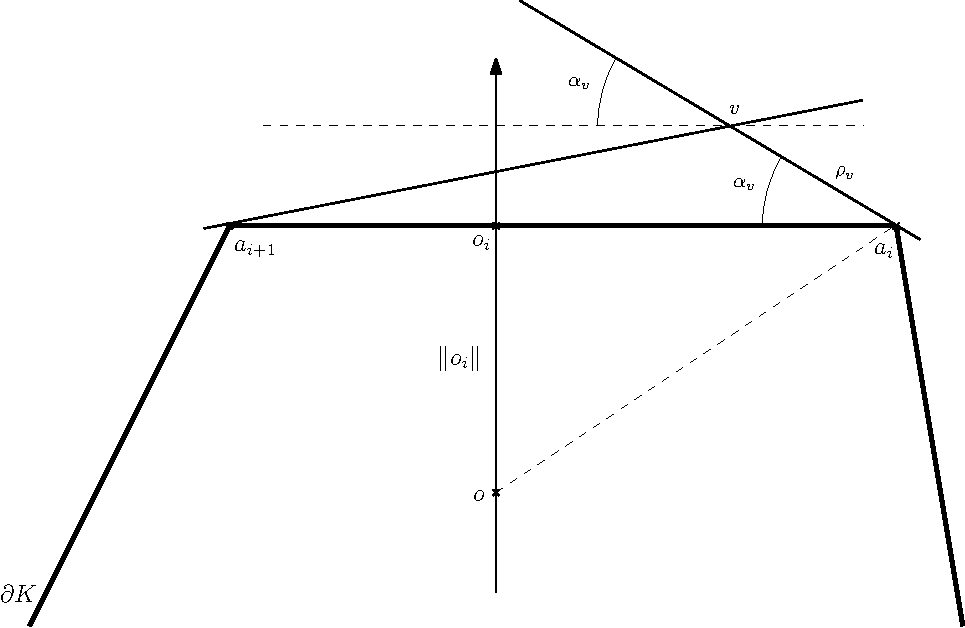
\includegraphics[scale=0.8]{sommetpolygon.pdf}
\caption{\label{fig:sommetpolygon}
Intensity of the point process of vertices near a fixed vertex $a_i$ of $K$.}
\end{figure}

%\noi
Thanks to Lemma~\ref{lem:geompoly1}, we get
\[
\Delta_i(\lambda,\rho,\alpha) \underset{\lambda\to\infty}{\longrightarrow} 2\|o_i\|\rho\alpha^2.
\]
Moreover,
\[
r_i(\lambda,\rho,\alpha) \underset{\lambda\to\infty}{\longrightarrow} \|a_i\|\,\text{ and }\,\sin(\theta_i(\lambda,\rho,\alpha)) \underset{\lambda\to\infty}{\longrightarrow} \frac{\|o_i\|}{\|a_i\|}.
\]

%\noi
Let us now turn on the term $J^{\supp}_i(\lambda,\rho,\alpha)$. We get successively
\begin{multline*}
J^{\supp}_i(\lambda,\rho,\alpha)\\
\begin{aligned}
& \underset{\lambda\to\infty}{\sim} \lambda^{3\gamma}\int_{\left(0,\lambda^{-\gamma}\alpha\right)^2} \left|\sin(\theta_i(\lambda,\rho,\alpha)-\theta_1)\sin(\theta_i(\lambda,\rho,\alpha)-\theta_2)\sin(\theta_2-\theta_1)\right|\dd \theta_1\dd \theta_2 \\
& \underset{\lambda\to\infty}{\sim} \lambda^{3\gamma}\left(\frac{\|o_i\|}{\|a_i\|}\right)^2 \left(\frac1{3}\left(\lambda^{-\gamma}\alpha\right)^3\right) = \frac1{3}\left(\frac{\|o_i\|}{\|a_i\|}\right)^2\alpha^3.
\end{aligned}
\end{multline*}

%\noi
We apply now again Lebesgue's dominated convergence theorem, omitting the domination step which is very similar to what we did in the proof of Proposition~\ref{prop:supportpoly}. It follows that
\[
\E(\cN_i(R\times A)) \underset{\lambda\to\infty}{\longrightarrow} 8\int_{R\times A} \exp\left(-2\|o_i\|\rho\alpha^2\right)\|a_i\|^2\times\frac1{3}\left(\frac{\|o_i\|}{\|a_i\|}\right)^2\alpha^3 \rho\dd\rho\dd\alpha
\]
which implies the required result.
\end{proof}
%$\square$



\section{Proof of Theorem~\ref{theo:steiner}: the role of the Steiner point}\label{sec:steiner}

%\noi
In the two previous sections, the cell that we considered is associated with a deterministic nucleus at the origin which is added to the Poisson point process. In particular, the asymptotic shape of the cell depends on both the choice of the convex body $K$ and the position of the origin $o$ inside $K$. In this section, we investigate a modified question which is intrinsic in $K$, i.e. we ask for the behavior of the cell ${K}_{\lambda}$ containing $K$ when the Poisson point process is conditioned on its associated Voronoi tessellation to not intersect $K$. Since the problem is invariant under translation, we are allowed to assume that the Steiner point of $K$ coincides with the origin, without it being a nucleus of the tessellation. More precisely, the Steiner point of $K$ denoted by $\st(K)$ is defined by the equality
\begin{equation*}
\st (K)=\frac{1}{\pi}\int_0^{2\pi} p_o(K,\theta)u_\theta\dd\theta.
\end{equation*}

%\noi
When $K$ is smooth, $\st (K)$ can be rewritten as
\begin{equation*}
\st (K)=\frac{1}{\pi}\int_{\partial K}r_s^{-1}\langle s,n_s\rangle n_s\dd s.
\end{equation*}

%\noi
In particular, $\st (K)$ is included in the relative interior of $K$, see e.g.~\cite[Section~1.7]{Schneider} for the definition and the general properties of $\st (K)$. Note in particular that its definition is intrinsic to $K$, i.e. is independent of the choice of the origin $o$. We show as a byproduct of the proof of Proposition~\ref{steinerpoint2} the alternative characterization of the Steiner point given in Proposition~\ref{prop:newcharac} below.

\begin{prop}\label{prop:newcharac}
The Steiner point $\st (K)$ is the unique point $x$ in $\R^2$ which minimises the function $x\longmapsto \cA(\cF_x(K))$.
\end{prop}

%\noi
Let $\scS_{\lambda}$ be the event such that there is one cell $\widehat{K}_\lambda$ of the Poisson--Voronoi tessellation associated with $\cP_{\lambda}$ which contains $K$. We are interested in showing that conditional on $\scS_{\lambda}$, the nucleus of $\widehat{K}_\lambda$, denoted by $Z_{\lambda}$, is close to the Steiner point $\st (K)$.

%\pass
The next proposition is an intermediary result which provides a precise description of the conditional distribution of $\cP_{\lambda}$ given $\scS_{\lambda}$ as well as the explicit and limit distributions for the rescaled nucleus of $K_{\lambda}$. Note that Proposition~\ref{steinerpoint2} combined with Theorem~\ref{theosmooth} will be the key tool for proving Theorem~\ref{theo:steiner}.

\begin{prop}\label{steinerpoint2}\ \\*[-1.45em]
%\noi
\begin{enumerate}\romanenumi
\item \label{prop5.2.1} The conditional distribution of $\cP_\lambda$ given $\scS_\lambda$ is equal in distribution to $\{Z_{\lambda}\}\cup \cP^{(Z_\lambda)}_\lambda$ where $Z_\lambda$ is a random variable distributed according to a density function proportional to $x\longmapsto\exp(-4\lambda\cA(\cF_x(K)))$ and, given $\{Z_{\lambda}=x\}$, $\cP^{(Z_\lambda)}_\lambda$ is a Poisson point process of intensity $\lambda{\emph{\indicat}}_{\R^2\setminus 2\cF_x(K)}$.
\item \label{prop5.2.2}Conditional on $\scS_{\lambda}$, the rescaled nucleus $\lambda^{\frac{1}{2}}Z_{\lambda}$ converges in distribution as $\lambda\to\infty$ to the centered Gaussian distribution with covariance matrix $(4\pi)^{-1}$ times the identity matrix.
\end{enumerate}
\end{prop}
\goodbreak

\begin{proof}[{Proof of Proposition~\ref{steinerpoint2}.}]

\begin{prooff}[{Proof of~\eqref{prop5.2.1}}]
Let $L$ be a fixed compact set in $\R^2$. Using Mecke--Slivnyak's\linebreak formula and denoting by $\cC_x$ the Voronoi cell associated with $x\in\R^2$, we get successively
\begin{align*}
\E\left(\indic_{\scS_{\lambda}}\indic_{\left\{\cP_{\lambda}\cap L=\emptyset\right\}}\right) & = \E\left(\sum_{x\,\in\,\cP_{\lambda}}\indic_{\left\{K\,\subset\,\cC_x\right\}}\indic_{\{\cP_{\lambda}\cap L\,=\,\emptyset\}}\right)\\
& =\int_{\R^2} \P\left(K\subset \cC_x,(\cP_{\lambda}\cup\{x\})\cap L=\emptyset\right)\dd x\\
& =\int_{\R^2\setminus L}\P\left(\cP_{\lambda}\cap (L\cup 2\cF_x(K))=\emptyset\right)\dd x\\
& =\int_{\R^2\setminus L}\exp\big(-\lambda\cA(L\setminus 2\cF_x(K))\big)\exp\big(-4\lambda\cA(\cF_x(K))\big)\dd x.
\end{align*}
Dividing the last equality by $\P(\scS_{\lambda})$, we get the required result.
\end{prooff}

\begin{lastprooff}[{Proof of~\eqref{prop5.2.2}}]
We start by calculating both $\P(\scS_{\lambda})$ and the density of $Z_{\lambda}$ conditional on $\scS_{\lambda}$. For any bounded and measurable function $\varphi:\R^2\longrightarrow \R$, we deduce from Mecke--Slivnyak's formula that
\begin{align*}
\E\left(\sum_{x\,\in\,\cP_{\lambda}}\indic_{\left\{K\subset \cC_x\right\}}\varphi(x)\right) &=\lambda\int_{\R^2} \P(K \subset \cC_x) \varphi(x) \dd x\\
 &=\lambda\int_{\R^2} \exp\big(-4\lambda\cA(\cF_x(K))\big) \varphi(x) \dd x.
\end{align*}

Taking $\varphi=1$ in the last equality above, we obtain that
\begin{equation*}
\P(\scS_{\lambda})=\lambda\int_{\R^2}\exp\big(-4\lambda\cA(\cF_x(K))\big)\dd x
\end{equation*}
and that the conditional density $f_{{\lambda}}$
of $\lambda^{\frac12}Z_{\lambda}$ is proportional to
\[
x\longmapsto\exp\big(-4\lambda\cA(\cF_{\lambda^{-1/2}x}(K))\big).
\]

%\pass
We now turn our attention to the calculation of $\cA(\cF_x(K))$. For any $x\in \R^2$, we denote by $\cE(x)\subset [0,2\pi]$ the set of all directions such that $p_x(K,\theta)> 0$. Denoting by
\begin{equation*}\label{eq:resteairefleur}
{\cT}(x)=\frac1{2}\int_{[0,2\pi]\setminus\cE(x)}p_x^2(K,\theta)\dd \theta,
\end{equation*}
we rewrite $\cA(\cF_x(K))$ as
\begin{equation*}
\cA(\cF_x(K)) =\frac1{2}\int_0^{2\pi}p_x^2(K,\theta)\dd\theta-{\cT}(x).
\end{equation*}

%s\noi
We notice that
\begin{equation}\label{eq:suppchangeref}
p_x(K,\theta) -p_o(K,\theta) = -\langle x, u_{\theta}\rangle.
\end{equation}
Consequently, we get
\begin{align}
\cA(\cF_x(K)) & =\frac1{2}\int_{0}^{2\pi} \left(p_o(K,\theta)-\langle x,u_{\theta}\rangle\right)^2\dd\theta-{\cT}(x)\nonumber\\
& =\cA(\cF_o(K))-\Big\langle x, \int_0^{2\pi} p_o(K,\theta)u_{\theta}\dd\theta\Big\rangle +\frac1{2}\int_0^{2\pi}\langle x,u_{\theta}\rangle^2\dd\theta-{\cT}(x)\nonumber\\
& =\cA(\cF_o(K))+\frac{\pi}{2}\|x\|^2-{\cT}(x)\label{eq:functionflower}
\end{align}
where we have used both the fact that $o$ is the Steiner point of $K$ and the equality
\begin{equation*}
\int_0^{2\pi}\langle x,u_{\theta}\rangle^2\dd\theta= \int_0^{2\pi}(\cos\theta)^2\|x\|^2\dd\theta =\pi \|x\|^2.
\end{equation*}

%\pass
Let us show two basic properties of the rest ${\cT}(x)$.
\begin{itemize}
\item[-] When $x$ is in the interior of $K$, $\cE(x)=[0,2\pi]$ and ${\cT}(x)=0$.
\item[-] When $x$ is not in the interior of $K$, because of~\eqref{eq:suppchangeref}, $0<p_o(K,\theta)\le \langle x,u_\theta\rangle$ as soon as $\theta\in [0,2\pi]\setminus\cE(x)$ and consequently, for any $\theta\in [0,2\pi]\setminus\cE(x)$,
\begin{equation*}
p_x(K,\theta)^2=\langle x,u_\theta\rangle^2-p_o(K,\theta)(2\langle x,u_\theta\rangle-p_o(K,\theta))\le \langle x,u_\theta\rangle^2.
\end{equation*}
\end{itemize}

%\pass
Combining this inequality with the fact that $[0,2\pi]\setminus \cE(x)$ is an interval of length at most $\pi$ implies in turn that
\begin{equation*}\label{eq:boundR(x)}
0\le {\cT}(x)\le \frac12\int_{[0,2\pi]\setminus\cE(x)} \langle x,u_\theta\rangle^2\dd\theta\le \frac{\pi}{4}\|x\|^2.
\end{equation*}
In view of~\eqref{eq:functionflower}, this means in particular that $o$ is the unique minimum of the function $x\longmapsto \cA(\cF_x(K))$.

%\pass
Now, inserting~\eqref{eq:functionflower} into the conditional density function $f_{\lambda}$ of $\lambda^{\frac12}Z_\lambda$, we obtain that $f_{\lambda}(x)$ is proportional to $\exp(-2\pi\|x\|^2+4\lambda{\cT}(\lambda^{-\frac12}x))$. Using the properties of $\cT$ detailed above and the fact that $\lambda^{-\frac{1}{2}}x$ lies in the interior of $K$ for $\lambda$ large enough, we get that for every $x\in\R^2$, $f_\lambda(x)$ converges to $2\exp(-2\pi\|x\|^2)$ and
\begin{equation*}
\exp\left(-2\pi\|x\|^2+4\lambda{\cT}\left(\lambda^{-\frac12}x\right)\right)\le \exp\left(-\pi\|x\|^2\right).
\end{equation*}

%\noi
Consequently, an application of Lebesgue's dominated convergence theorem shows that for any measurable function $g:\R^2\longrightarrow \R$ which is bounded by a polynomial of~$\|x\|$,
\begin{equation*}
\int_{\R^2} g(x)f_\lambda(x)\dd x \underset{\lambda\to\infty}{\longrightarrow} 2\int_{\R^2} g(x)\exp(-2\pi\|x\|^2)\dd x
\end{equation*}
which completes the proof of Proposition~\ref{steinerpoint2}.
\end{lastprooff}\let\qed\relax
\end{proof}
%$\square$

%\pass
We are now ready to prove Theorem~\ref{theo:steiner}.

\begin{proof}[{Proof of Theorem~\ref{theo:steiner}}]
We prove the result for $\E(\cA(K_\lambda))-\cA(K)$ and explain at the end how to adapt the arguments for $\E((\cU(K_\lambda))-\cU(K)$ and $\E(\cN(K_\lambda))$.

Let $\cC_o$ be the Voronoi cell associated with the origin when $o$ is added to the set of nuclei $\cP_\lambda$. The cell $K_{\lambda}$ containing $K$ is distributed, up to a translation, as $\cC_o$ conditional on $(K+Z_{\lambda})\subset \cC_o$, where $Z_{\lambda}$ is distributed as in Proposition~\ref{steinerpoint2}$\MK$\eqref{prop5.2.1}. Recalling that $f_{\lambda}$ is the density function of $\lambda^{\frac12}Z_\lambda$, we obtain
\begin{align*}
\E(\cA(K_\lambda)-\cA(K)) &= \int_{\R^2}\E\left(\cA((K+\lambda^{-\frac{1}{2}}x)_\lambda^o )-\cA(K)\right)f_{\lambda}(x)\dd x = I_1(\lambda)+I_2(\lambda)
\\
\intertext{where}
I_1(\lambda) & =\int_{\lambda^{\frac14}K}\E\left(\cA((K+\lambda^{-\frac{1}{2}}x)_\lambda^o)-\cA(K)\right)f_{\lambda}(x)\dd x \\
\intertext{and} \\
I_2(\lambda) & =\int_{\R^2\setminus\lambda^{\frac14}K}\E\left(\cA((K+\lambda^{-\frac{1}{2}}x)_\lambda^o)-\cA(K)\right)f_{\lambda}(x)\dd x\,.
\end{align*}

%\pass
We start by showing that
\begin{equation}\label{eq:convI1}
I_1(\lambda)\underset{\lambda\to\infty}{\sim}\E\left(\cA({K}_\lambda^o)-\cA(K)\right).
\end{equation}
Indeed, a method similar to what has been done in Sections~\ref{subsec:surfacesmooth} and~\ref{subsec:surfacepolygon} shows that, uniformly in $x\in\R^2$,
\begin{equation*}
\E\left(\cA((K+\lambda^{-\frac1{2}}x)_\lambda^o)-\cA(K)\right)\indicat_{\left\{x\,\in\,\lambda^{\frac14}K\right\}}\underset{\lambda\to\infty}{\sim}\E\left(\cA({K}_\lambda^o)-\cA(K)\right).
\end{equation*}
Combining this with the convergence and domination of the function $f_\lambda$ showed in the proof of Proposition~\ref{steinerpoint2}$\MK$\eqref{prop5.2.2}, we get~\eqref{eq:convI1}.

%\pass
Let us show now that the integral $I_2(\lambda)$ is negligible in front of $I_1(\lambda)$. To do so, we denote by $R_x$ the maximal distance from $o$ to the farthest point in $(K+\lambda^{-\frac12}x)_\lambda^o$. We notice in particular that $\cA((K+\lambda^{-\frac1{2}}x)_\lambda^o)\le \pi R_x^2$. Moreover, by a method similar to Lemma~$1$ in~\cite{fs96}, we obtain that, for any $r>0$,
\[
\P\left(R_x\ge r\right)\le C'\exp\left(-Cr^2+C'\lambda^{-1}\|x\|^2\right),
\]
for some positive constants $C,C'>0$.

%\noi
Consequently, $\E(\cA((K+\lambda^{-\tfrac1{2}}x)_\lambda^o)-\cA(K))$ is bounded by $1+\lambda^{-1}\|x\|^2$ up to a multiplicative constant. Using the domination of $f_\lambda$ showed in Proposition~\ref{steinerpoint2}$\MK$\eqref{prop5.2.2}, we get that $I_2(\lambda)\to 0$ exponentially fast as $\lambda\to\infty$. Combining this last result with~\eqref{eq:convI1}, we obtain the required convergence for the mean defect area of $K_\lambda$.

%\pass
Finally, the estimates for $\E(\cU(K_\lambda)-\cU(K))$ and $\E(\cN(K_\lambda))$ follow from similar arguments, as soon as we are able to get bounds for $\E(\cU((K+\lambda^{-\frac1{2}}x)_\lambda^o)-\cU(K))$ and $\E(\cN((K+\lambda^{-\frac1{2}}x)_\lambda^o))$. Using the inclusion $(K+\lambda^{-\frac12}x)_\lambda^o\subset B_o(R_x)$, we get that, up to a multiplicative constant, $\lambda^{-\frac12}\|x\|$ is an upper-bound of $\E(\cU((K+\lambda^{-\frac{1}{2}}x)_\lambda^o))-\cU(K))$. A use of Proposition~\ref{prop:efron}$\MK$\eqref{prop2.1.i} combined with the same inclusion finally shows that, up to a multiplicative constant, $\lambda^{-1}\|x\|^2$ is an upper-bound of $\E(\cN((K+\lambda^{-\frac1{2}}x)_\lambda^o))$.
\end{proof}
%$\square$



\section{Proof of Theorem~\ref{theo:var}: the question of the variance}\label{sec:variancesmooth}

%\noi

In this section, we explain how a general method based on the application of an inversion with respect to the osculating disk at $s$ for any $s\in\partial K$ provides an explicit calculation of the limiting variance of the defect area and the number of vertices in the smooth case. As in Theorem~\ref{theo:steiner}, these results extend to $K_\lambda$.

\begin{proof}[{Proof of Theorem~\ref{theo:var}}]
Compared to the direct calculations done in the previous sections, the method used in this proof is clearly more technical and relies on previous works for random convex hulls. Similar arguments could have also led to Theorem~\ref{theosmooth} but we had chosen to keep the discussion as plain as possible for the expectation asymptotics, which seems to be no longer possible for the variance asymptotics. The technique described below is reminiscent of both~\cite{cs05} for the idea of transforming through the action of an inversion a Voronoi cell into a convex hull and~\cite{cy14} for the rewriting of the variance as an integral over $\partial K$ of a covariance of so-called \emph{scores} and the replacement of $K$ by a disk in the calculation of these scores. Though it is specific to the smooth case and can hardly be extended to the variance of the perimeter, it may also reinforce the parallel with R\'enyi and Sulanke's work and explain to some extent why these particular functionals of $K$ appear in the limiting expectations and variances.

%\pass
We describe in detail the technique in the case of $\cN(K_{\lambda}^o)$ and explain at the end how to extend it for the defect area. The first step consists in associating to any $x\in \cP_\lambda\setminus 2\cF_o(K)$ the point $y$ which is the closest point to $\partial K$ on the bisecting line of the segment $[0,x]$. We denote by $\cQ_\lambda$ the point process constituted of the coordinates $(s,h)$ of such points $y$. In particular, $\cQ_\lambda$ is a Poisson point process on $\partial K\times (0,\infty)$ and its intensity with respect to the measure $\dd s\dd h$ has a density equal to $q_{\lambda}(s,h)=4\lambda r_s^{-1}(\langle s,n_s\rangle +h)$ thanks to the equalities $\|x\|=2(\langle s,n_s\rangle+h)$ and $\tfrac{\dd s}{\dd\theta}=r_s$ (see also Figure~\ref{fig:dessinQlambda}).

\begin{figure}[h!]
\begin{center}
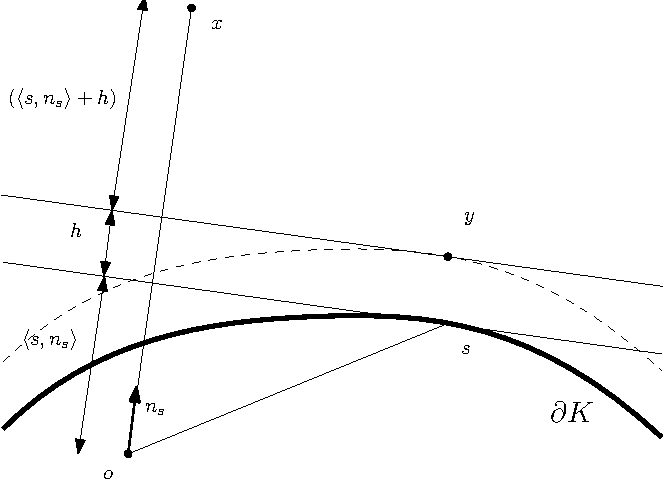
\includegraphics[scale=1]{dessinQlambda.pdf}
\end{center}
\caption{The construction of the point $y\in \cQ_\lambda$ associated with $x\in \cP_\lambda$}\label{fig:dessinQlambda}
\end{figure}

%\pass
 For every $(s,h)\in \cQ_\la$, we denote by $\xi((s,h),\cQ_\la)$ the score of $(s,h)$, equal to either $1$ if its ancestor in $\cP_\lambda$ is a Voronoi neighbor of $o$ and $0$ otherwise. In particular,
\[
{\cN}(K_{\lambda}^o)=\sum_{(s,h)\,\in\,\cQ_\la} \xi\left((s,h),\cQ_\la\right)\,.
\]
Consequently, using the Mecke--Slivnyak's formula, we get that
\begin{align}
&\la^{-\frac{1}{3}}\Var(\cN(K_{\lambda}^o))\nonumber\\
=&\la^{-\frac{1}{3}}\E\left(\sum_{(s,h)\,\in\, \cQ_\la}\xi^2((s,h),\cQ_\la)+\sum_{(s,h)\,\ne\, (s',h')\,\in\, \cQ_\la}\xi\left((s,h),\cQ_\la\right)\xi\left((s',h'),\cQ_\la\right)\right)\nonumber\\
-&\la^{-\frac{1}{3}}\left(\E(\cN(K_{\lambda}^o))\right)^2=I_{1,\lambda}+I_{2,\lambda}\label{eq:decompvar}
\end{align}
where
\begin{align*}
I_{1,\lambda}&=\lambda^{-\frac{1}{3}}\int_{\partial K\times (0,\infty)}\E\left(\xi^2((s,h),\cQ_\la)\right)q_\lambda(s,h)\dd s\dd h,\\
I_{2,\lambda}&=\lambda^{-\frac{1}{3}}\iint_{(\partial K\times (0,\infty))^2}c\left((s,h),(s',h'),\cQ_\la\right)q_\lambda(s,h)q_\lambda(s',h')\dd s\dd h\dd s'\dd h'
\end{align*}
and $c$ denotes the pair correlation function defined as
\begin{align*}
c\left((s,h),(s',h'),\cP_\la\right)&=\E\Big(\xi\big((s,h),\cQ_\la\cup\{(s',h')\}\big)\xi\big((s',h'),\cQ_\la\cup\{(s,h)\}\big)\Big)\\
&\quad-\E\big(\xi((s,h),\cQ_\la)\big)\E\big(\xi((s',h'),\cQ_\la)\big).
\end{align*}

%\noi
Let us denote by $\cI_s$ the renormalized inversion with respect to the center of curvature $\omega_s$ defined by the identity
\[
\cI_s(y)=\omega_s+r_s\frac{y-\omega_s}{\|y-\omega_s\|^2},\quad y\ne \omega_s.
\]
The image $\widetilde{\cQ}_{\la,\,s}=\cI_s(\cQ_\la)$ is a Poisson point process in the osculating disk $B_{r_s}(\omega_s)$ at $s$, which has a density $\widetilde{q}_{\lambda,s}(r,\theta)$ with respect to the polar coordinates, equivalent to $4\lambda r_s\langle s,n_s\rangle$ when $(r,\theta)\to (1,0)$. Moreover, the same arguments as in~\cite[Lemma~1]{cs05} show that the new score $\widetilde{\xi}((r,\theta),\widetilde{\cQ}_{\la,s})=\xi(\cI_s^{-1}(\omega_s+ru_{\theta}),\cQ_\la)$, $(r,\theta)\in (0,1)\times(0,2\pi)$, is equal to $1$ if $(r,\theta)$ is an extreme point of $\widetilde{\cQ}_{\la,\,s}\cup\{(r,\theta)\}$ and $0$ otherwise. In the same way, we define the new pair correlation function $\widetilde{c}((r,\theta), (r',\theta'),\widetilde{\cQ}_{\la,s})$. Applying the change of variables $r=\frac{r_s}{r_s+h}$ in $I_{1,\,\lambda}$ which means taking $r$ for the distance between $\omega_s$ and the image by $\cI_s$ of $(s,h)$, we obtain that
\[
I_{1,\lambda}= \lambda^{-\frac{1}{3}}\int_{\partial K}\int_{r\,\in\,(0,1)}\E\left(\widetilde{\xi}^2\left((r,0),\widetilde{\cQ}_{\la,s}\right)\right)4\lambda r_s^{-1}\left(\left\langle s,n_s\right\rangle+\frac{r_s}{r}-r_s\right)\frac{r_s}{r^2}\dd r\dd s.
\]

%\noi
Let us define $\varepsilon_\la=(\tfrac{\log \lambda}{\lambda})^{-\frac13}$. We claim that with high probability, only the values of $r$ close to $1$ up to a distance of order $\Odd(\varepsilon_\lambda^2)$ will contribute significantly to the integral above and moreover, that only the points of $\widetilde{\cQ}_{\la,s}$ at a distance $\Odd(\varepsilon_\lambda)$ will be needed for the computation of the scores. Indeed, this is due to a result which can be proved analogously to~\cite[Lemma~4.1$\MK$(a), Lemma~4.2]{cy14} and which says the following: there exists a positive constant $C$ such that with probability $(1-\Odd(\lambda^{-8}))$,
\[
\widetilde{\xi}\left((r,0),\widetilde{\cQ}_{\la,s}\right)=
\begin{cases}
\widetilde{\xi}\left((r,0),\widetilde{\cQ}_{\la,s}\cap B_{C\varepsilon_\la}(s)\right)& \text{if }r\ge 1-C\varepsilon_\la^2\\
0 & \text{otherwise}.
\end{cases}
\]
Note that~\cite{cy14} assumes a $\cC^3$-smooth boundary but that in particular, Lemmas~4.1 and 4.2 therein still hold with the weaker assumption of $\cC^2$-regularity. Recalling now that when $(r,\theta)\to (1,0)$, the intensity of $\widetilde{\cQ}_{\la,s}$ goes to $4\lambda r_s\langle s,n_s\rangle$, we obtain that
\begin{equation}\label{eq:I1lambdaok}
I_{1,\,\lambda} \underset{\lambda\to\infty}{\sim}\lambda^{-\frac13}
\int_{\partial K}r_s^{-1}\cdot 4\lambda r_s\langle s,n_s\rangle
\int_{0}^1\E\left(\widetilde{\xi}^2\left((r,0),\cP_{4\lambda r_s\langle s,n_s\rangle}\cap B_1(o)\right)\right)\dd r \dd s.
\end{equation}

%\noi
We proceed analogously for $I_{2,\lambda}$, i.e. we apply the two changes of variables $r=\tfrac{r_s}{r_s+h}$ and $(r',\theta')$ as the polar coordinates with respect to $\omega_s$ of the image by $\cI_s$ of the point $(s',h')$. Using that with high probability $\widetilde{\xi}((r,0),\widetilde{\cQ}_{\la,s})=0$ as soon as $r$ exceeds $\Odd((\tfrac{\log \lambda}{\lambda})^{-\frac23})$ and that $\widetilde{c}((r,0),(r',\theta'),\widetilde{\cQ}_{\la,s})=0$ as soon as the distance between the two points with polar coordinates $(r,0)$ and $(r',\theta')$ exceeds $\Odd((\tfrac{\log \lambda}{\lambda})^{-\frac23})$, see~\cite[Lemma~4.1]{cy14}, we obtain that
\begin{equation}\label{eq:I2lambdaok}
\begin{aligned}
\lambda^{\frac{1}{3}}I_{2,\lambda}
=&\int_{\partial K} \int_{r,r'\,\in\,(0,1),\theta'\in(0,2\pi)}\widetilde{c}\left((r,0),(r',\theta'),\widetilde{\cQ}_{\la,s}\right)4\lambda \left(\langle s,n_s\rangle
+\frac{r_s}{r}-r_s\right)\\
&\widetilde{q}_{\la,s}(r',\theta')\frac{\dd r}{r^2}\dd r'\dd \theta'\dd s
\underset{\lambda\to\infty}{\sim}\int_{\partial K} r_s^{-1}\cdot \left(4\lambda r_s\langle s,n_s\rangle\right)^2\\
&\int_{r,r'\,\in\,(0,1),\theta'\,\in\,(0,2\pi)}\widetilde{c}\left((r,0),(r',\theta'),\cP_{4\lambda r_s\langle s,\,n_s\rangle}\cap B_1(o)\right)\dd r\dd r'\dd\theta'\dd s.
\end{aligned}
\end{equation}

%\noi
Using~\cite[Theorem~7.1]{CSY}, we have for fixed $s\in \partial K$
\begin{multline}\label{eq:limvarenvconv}
\lim_{\la\to\infty} (4\lambda r_s\langle s,n_s\rangle)^{-\frac13}\left(4\lambda r_s\langle s,n_s\rangle\int_{0}^1\E\left(\widetilde{\xi}^2((r,0),\cP_{4\lambda r_s\langle s,n_s\rangle}\cap B_1(o))\right)\dd r\right.\\
\left.+(4\lambda r_s\langle s,n_s\rangle)^2\!\!\int_{r,r'\,\in\,(0,1),\theta'\,\in\,(0,2\pi)}\!\widetilde{c}\left(\!(r,0),(r',\theta'),\cP_{4\lambda r_s\langle s,n_s\rangle}\cap B_1(o)\!\right)\dd r\dd r'\dd\theta'\!\!\right)\!=\frac{c_{\cN}}{2\pi}
\end{multline}
where $c_{\cN}$ is the positive limiting variance of the number of extreme points of a homogeneous Poisson point process inside the unit disk. Combining~\eqref{eq:limvarenvconv} with~\eqref{eq:decompvar}, \eqref{eq:I1lambdaok} and~\eqref{eq:I2lambdaok}, we obtain Theorem~\ref{theo:var}$\MK$\eqref{theo1.5.ii}.

%\pass
Regarding the variance of $\cA(K_{\lambda}^o)$, we proceed in the exact same way, the only notable difference being that we take $\xi((s,h),\cQ_\lambda)$ equal to the area between $\partial K$ and the Voronoi edge contained in the bisecting line that $(s,h)$ belongs to if such Voronoi edge exists and $0$ otherwise, see the hatched region in Figure~\ref{fig:scoreaire}$\MK$(a). Denoting by $\mu_s$ the image of the Lebesgue measure by $\cI_s$, is also equal to the $\mu_s$-measure of the hatched region on Figure~\ref{fig:scoreaire}$\MK$(b) when $(r,0)$ is an extreme point of $\widetilde{\cQ}_{\la,s}\cap B_1(o)$ and $0$ otherwise. Since with high probability this hatched region is very close to the boundary of $B_1(o)$, the $\mu_s$-measure is almost equal to $r_s^{2}$ times the Lebesgue measure. Consequently, we choose for $\widetilde{\xi}((r,0),\widetilde{\cQ}_{\la,s})$ the Lebesgue measure of the hatched region and define $\widetilde{c}$ accordingly.

%%Subfigure ici!
\begin{figure}
\centering
\begin{tabular}{ccc}
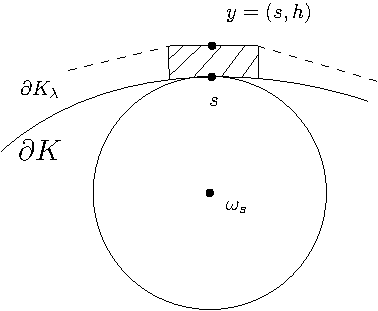
\includegraphics[scale=1]{xiairebase.pdf} & \hspace*{1cm} &
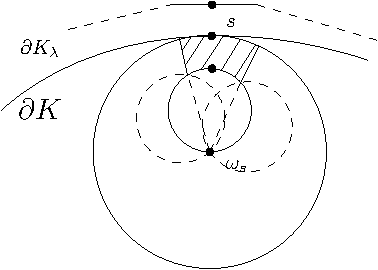
\includegraphics[scale=1]{xiaireinverse.pdf}\\
\hspace*{1cm}(a) & & \hspace*{1cm}(b)
\end{tabular}
\caption{The two scores $\xi$ (a) and $\widetilde{\xi}$ (b) for the variance of $\cA(K_{\lambda}^o)$}\label{fig:scoreaire}
\end{figure}

%\pass
Thanks to~\cite[Theorem~7.1]{CSY}, we get that
\begin{multline}\label{eq:limvarenvconv2}
\lim_{\la\to\infty} (4\lambda r_s\langle s,n_s\rangle)^{\frac53}\left(4\lambda r_s\langle s,n_s\rangle\int_{0}^1\E\left(\widetilde{\xi}^2((r,0),\cP_{4\lambda r_s\langle s,n_s\rangle}\cap B_1(o))\right)\dd r\right.\\
\left.+(4\lambda r_s\langle s,n_s\rangle)^2\int_{r,r'\,\in\,(0,1),\theta'\,\in\, (0,2\pi)}\widetilde{c}((r,0),(r',\theta'),\cP_{4\lambda r_s\langle s,n_s\rangle}\cap B_1(o))\dd r\dd r'\dd \theta'\right)\!=\frac{c_{\cA}}{2\pi}
\end{multline}
where $c_{\cA}$ is the positive limiting variance of the area between the boundary of $B_1(o)$ and the Voronoi flower of a homogeneous Poisson point process inside the unit disk. Incidentally, this quantity is also the limiting variance of $\pi$ times the mean width of the convex hull of the same homogeneous Poisson point process. Finally, \eqref{eq:limvarenvconv2} combined with the fact that $\Var(\cA(K_{\lambda}^o))$ is equivalent to the integral over $\partial K$ of\linebreak$r_s^3$ times the quantity inside the brackets in~\eqref{eq:limvarenvconv2} implies Theorem~\ref{theo:var}$\MK$\eqref{theo1.5.i}.
\end{proof}

%\pass
A byproduct of the method developed in the proof of Theorem~\ref{theo:var} is that
\begin{align*}
\E(\cA(K_{\lambda}^o))-\cA(K) &\underset{\lambda\to\infty}{\sim} \lambda^{-\frac{2}{3}} 2^{-\frac73} a_\infty\displaystyle\int_{\partial K} r_s^{\frac1{3}}\left\langle s,n_s\right\rangle^{-\frac{2}{3}}\dd s
\\
\intertext{and}
\E(\cN(K_{\lambda}^o))&\underset{\lambda\to\infty}{\sim} \lambda^{\frac{1}{3}}2^{-\frac13}\pi^{-1} n_\infty \displaystyle\int_{\partial K} r_s^{-\frac{2}{3}}\left\langle s,n_s\right\rangle^{\frac1{3}}\dd s
\end{align*}
where $a_\infty$ (resp. $n_\infty$) is the normalized limiting expectation of the defect mean width (resp. number of vertices) of the convex hull of a homogeneous Poisson point process in the unit disk.

%\pass
Using~\cite[Satz~3]{resu63} and~\cite[Satz~1]{resu64}, the two equalities above imply points~\eqref{theo1.1.i} and~\eqref{theo1.1.iii} of Theorem~\ref{theosmooth}. Nevertheless, we have chosen to prove them in Section~\ref{sec:smooth} through a direct calculation instead because it is more natural and self-contained on one hand and easier to extend to the defect perimeter and to the polygonal case on the other hand. Besides, the method used in Section~\ref{sec:smooth} implies Proposition~\ref{prop:supportsmooth} on the support points which is new to the best of our knowledge and interesting on its own.


%\pass
The extension of the method from Section~\ref{sec:variancesmooth} to the case of the perimeter is indeed problematic. This comes from the fact that it relies in particular on the application of an inversion with respect to an osculating circle of $K$ and the use of the known asymptotics for a random convex hull inside a disk. There have been in the past successful uses of the polarisation of a convex body in order to derive asymptotics for the perimeter or mean width of random convex hulls, see e.g.~\cite{gg97,br04}. Only understanding how this transition to the polar body would impact the construction of the Poisson--Voronoi cell seems non-trivial. This could suggest that we should adapt the technique of~\cite{cy14} without any use of an inversion or a polarisation, i.e. show the existence of a scaling limit of the boundary of the Voronoi tessellation in the osculating disk and define limiting scores associated with the defect perimeter in the rescaled space. This program seems reachable for both the limiting expectation and limiting variance of the defect perimeter, though it would not provide any explicit calculation of the constants involved, contrary to Theorem~\ref{theosmooth}$\MK$\eqref{theo1.1.ii}. We leave it for future research.

%\pass
We believe that the extension to higher dimension of the method from Section~\ref{sec:variancesmooth} is delicate and would require a non-trivial input which is still unclear up to now. Indeed, the technique relies on the approximation of the boundary of $K$ near a boundary point by an osculating circle, then on the use of the inversion transformation and the required asymptotic result for the convex hull of a random set of points in the disk. In higher dimension, the boundary of $K$ is locally approximated by an ellipsoid. In the case of the convex hull of a Poisson point process, \cite{cy14} settles that problem by applying a volume-preserving affine transformation so that the principal curvatures of $K$ at a fixed boundary point are all equal. This does not modify the set of extreme points, as well as the defect volume of the random convex hull. The considered functionals, number of $k$-dimensional faces and defect volume, are then estimated inside an \emph{osculating ball} where there are an available global scaling transformation and asymptotics ready for use, see e.g.~\cite{CSY,cy14}. But in our case, the Voronoi construction is not preserved by the application of an affine transformation which is not isometric. Up to now, we have not been able to overcome this new difficulty.

%\pass
Regarding the polygonal case, there is no easy transformation which could play the role of the inversion, i.e. send the Voronoi cell to the convex hull of a random set of points inside the polygon and allow us then to use the known results on the random convex hull. A direct proof designed to mimic the strategy of~\cite{cy17} would induce many technical results currently missing (negligibility of the flat parts, decorrelation of the parts around the vertices of the polygon). Moreover, it could very well crash into the problem of defining a universal scaling transformation in the vicinity of a vertex of the polygon since the affine transformations do not preserve the Voronoi construction.



\section{The Crofton cell}\label{sec:crofton}

%\noi
The main issues of the paper prove to be equally appealing when the Poisson--Voronoi tessellation is replaced by any random line tessellation in the plane and in particular by the stationary and isotropic Poisson line tessellation, see e.g.~\cite[Section~10.3]{SW}. This tessellation is obtained by taking a Poisson point process $\overline{\cP}_\lambda$ of intensity measure $\lambda \|x\|^{-1}\dd x$ in $\R^2$ and constructing for every $x$ in the point process, the line $L_{x}$ containing $x$ and with normal vector $x$. The cell containing the origin is the so-called \emph{Crofton cell} and is defined as the intersection of all closed half-planes containing the origin and delimited by lines $L_{x}$. We denote by $\overline{K}_\lambda$ a cell distributed as the Crofton cell conditional on the event that no line crosses $K$, which is equivalent to say that no point from $\overline{\cP}_\lambda$ meets $\cF_o(K)$. We recall that thanks to the Cauchy-Crofton formula, this event has probability
\begin{align}
\exp\left(-\lambda\int_{\cF_o(K)}\|x\|^{-1}\dd x\right)&=\exp\left(-\lambda\int_{0}^{2\pi}\int_0^{p_o(K,\theta)}r^{-1}r\dd r \dd \theta\right)\nonumber\\
&=\exp\left(-\lambda\int_{0}^{2\pi}p_o(K,\theta)\dd \theta\right)\nonumber
\\
&=\exp(-\lambda\cU(K)).\label{eq:probavidecrofton}
\end{align}


%\noi
This new random polygon $\overline{K}_{\lambda}$ satisfies~\eqref{eq:croftonperimeter} and its rewritings given in Corollary~\ref{coro:appliEfronsmooth} (i) for the smooth case and in Corollary~\ref{coro:appliEfronpolygonal} for the polygonal case. The identity~\eqref{eq:airesmooth} is replaced by
\begin{align}\label{eq:defectareacrofton}
\E(\cA(\overline{K}_\lambda))-\cA(K) =\int_{\R^2\setminus K} \exp\Big(-\lambda (\cU(\conv(K\cup\{x\}))-\cU(K))\Big)\dd x.
\end{align}

%\noi
We state below the direct analogues for $\overline{K}_\lambda$ of Proposition~\ref{prop:efron}, Theorems~\ref{theosmooth} and~\ref{theopolygon} with the same notation. In particular, the Efron-type identity given at (a) can be seen as a consequence of~\cite[penultimate display on page 693]{Sch09}.

\goodbreak
\begin{theo}\label{theo:crofton}\ \\*[-1.4em]
\begin{enumerate}\alphenumi
\item \label{theo7.1.a}For every $\lambda>0$, the following identity holds
\begin{equation*}
\E(\cN(\overline{K}_\lambda))=\lambda(\E(\cU(\overline{K}_\lambda))-\cU(K))\,.
\end{equation*}
\pagebreak
\item\label{theo7.1.b} Let $K$ be a smooth convex body containing $o$ in its interior. The mean defect area, defect perimeter and number of vertices of $K_{\lambda}^o$ have respectively the following asymptotics when the intensity $\lambda\to\infty$:
\begin{align}
\tag{$\rm i$}\label{theo7.1.b.1} \E(\cA(\overline{K}_{\lambda}))-\cA(K) &\underset{\lambda\to\infty}{\sim} \lambda^{-\frac{2}{3}}2^{-\frac{2}{3}}3^{-\frac1{3}}\Gamma\Big(\mfrac{2}{3}\Big)
 \int_{\partial K}r_s^{\frac1{3}} \dd s\\
\tag{$\rm ii$}\label{theo7.1.b.2} \E(\cU(\overline{K}_{\lambda}))-\cU(K) &\underset{\lambda\to\infty}{\sim}
\lambda^{-\frac{2}{3}}2^{\frac43}3^{-\frac{4}{3}}\Gamma\Big(\mfrac{2}{3}\Big)
\int_{\partial K} r_s^{-\frac{2}{3}}\dd s \\
\tag{$\rm iii$}\label{theo7.1.b.3} \E(\cN(\overline{K}_\lambda)) &\underset{\lambda\to\infty}{\sim} \lambda^{\frac1{3}}2^{\frac43}3^{-\frac{4}{3}}\Gamma\Big(\mfrac{2}{3}\Big)
\int_{\partial K} r_s^{-\frac{2}{3}}\dd s.
\end{align}

\item\label{theo7.1.c} Let $K$ be a convex polygon containing $o$ in its interior. The mean defect area, defect perimeter and number of vertices of $K_{\lambda}^o$ have respectively the following asymptotics when the intensity $\lambda\to\infty:$
\begin{align}
\tag{$\rm i$}\label{theo7.1.c.1} \E(\cA(\overline{K}_\lambda))-\cA(K) &\underset{\lambda\to\infty}{\sim}\lambda^{-\frac1{2}}\displaystyle 2^{-\frac{5}{2}}\pi^{\frac{3}{2}} \sum_{i=1}^{n_K} \|a_{i+1}-a_i\|^{\frac{3}{2}} \\
\tag{$\rm ii$}\label{theo7.1.c.2} \E(\cU(\overline{K}_{\lambda}))-\cU(K) &\underset{\lambda\to\infty}{\sim} (\lambda^{-1}\log \lambda)\cdot2\cdot 3^{-1}n_K \\
\tag{$\rm iii$}\label{theo7.1.c.3} \E(\cN(\overline{K}_\lambda)) &\underset{\lambda\to\infty}{\sim}(\log\lambda)\cdot2\cdot 3^{-1}n_K.
\end{align}
\end{enumerate}
\end{theo}

\begin{proof}[{Proof of Theorem~\ref{theo:crofton}}]
As all these results can be derived in a very similar way to what we did in the previous sections, we only sketch the proof below.
\begin{itemize}
\item[\eqref{theo7.1.a}] As in Proposition~\ref{prop:efron}, we observe that $x\in \overline{\cP}_\lambda$ gives birth to a side of the Crofton cell $\overline{K}_{\lambda}$ if and only if $L_x$ intersects the Crofton cell $\overline{C}_x$ corresponding to the point process ($\overline{\cP}_\lambda\setminus \cF_o(K))\setminus\{x\}$. This is equivalent to saying that $x\in {\cF}_o(\overline{C}_x)\setminus\cF_o(K)$. We then conclude by using Mecke--Slivnyak's formula combined with~\eqref{eq:probavidecrofton}.\\

\item[\eqref{theo7.1.b}$\MK$\eqref{theo7.1.b.1}] We need an analogue of Lemma~\ref{lem:geom} for the quantity $\cU(K\cup\{s_h\})-\cU(K)$ where we recall that $s_h=s+hn_s$ for any $s\in \partial K$ and $h>0$. Using the Cauchy--Crofton formula, we get with the same notation as in the proof of Lemma~\ref{lem:geom}
\begin{equation}\label{eq:defectperimeter}
\cU(K\cup\{s_h\})-\cU(K) =\int_{-\theta_{s,h}^-}^{\theta_{s,h}^+}\Delta p_{\omega_s}(\theta)\dd\theta
\underset{h\to 0}{=}2^{\frac{5}{2}}3^{-1}\, r_s^{-\frac1{2}} h^{\frac{3}{2}}+ \od\left(h^{\frac32}\right).
\end{equation}
We then insert~\eqref{eq:defectperimeter} into~\eqref{eq:defectareacrofton} and apply Lebesgue's dominated convergence theorem.
\pagebreak

\item[\eqref{theo7.1.b}$\MK$\eqref{theo7.1.b.2}] We start by stating an analogue of Proposition~\ref{prop:supportsmooth}: denoting by $(\overline{X}_{s,\lambda},\overline{Y}_{s,\lambda})$ the support point of $\partial \overline{K}_{\lambda}$ in direction $n_s$, we can show that the couple $(\lambda^{\frac1{3}}\overline{X}_{s,\lambda}, \lambda^{\frac{2}{3}}\overline{Y}_{s,\lambda})$ converges in distribution to the distribution with density function equal to
\[
2^{\frac{3}{2}} r_s^{-\frac{3}{2}}\exp\left(-2^{\frac{5}{2}} 3^{-1}r_s^{-\frac1{2}}
\left(\frac{x^2}{2r_s}+y\right)^{\frac{3}{2}}\right)\left(\frac{x^2}{2r_s}+y\right)^{\frac1{2}}y{\emph{\indicat}}_{\{y\,>\,0\}}.
\]
In particular, this implies
\begin{equation}\label{eq:espasympybarre}
\E(\overline{Y}_{s,\lambda})\underset{\lambda\to\infty}{\sim}\lambda^{-\frac{2}{3}}2^{\frac43}3^{-\frac{4}{3}}\Gamma\Big(\mfrac{2}{3}\Big) r_s^{\frac1{3}}.
\end{equation}
Inserting~\eqref{eq:espasympybarre} into the equality~\eqref{coro2.2.1} from Corollary~\ref{coro:appliEfronsmooth} applied to $\overline{K}_{\lambda}$, we get the required result.\\

\item[\eqref{theo7.1.c}$\MK$\eqref{theo7.1.c.1}] We prove an analogue of Lemma~\ref{lem:geompoly1} for the quantity $\cU(K\cup\{s_{a_i,\rho,\alpha}\})-\cU(K)$ for $s_{a_i,\rho,\alpha}\in \cS_i$ where we recall that $s_{a_i,\rho,\alpha}=a_i+\rho u_{\pi-\alpha}$. We get
\begin{align}
&\cU(K\cup\{s_{a_i,\rho,\alpha}\})-\cU(K)\nonumber\\
&=\|a_i-s_{a_i,\rho,\alpha}\|+\|a_{i+1}-s_{a_i,\rho,\alpha}\|-\|a_{i+1}-a_i\|\nonumber\\
&=\rho+\left(\rho^2+\|a_{i+1}-a_i\|^2-2\rho\|a_{i+1}-a_i\|\cos\alpha\right)^{\frac12}-\|a_{i+1}-a_i\|
\nonumber\\
&\!\!\underset{\alpha\to 0}{=}\frac{\alpha^2}{2}\frac{\rho\|a_{i+1}-a_i\|}{\|a_{i+1}-a_i\|-\rho}+\od\left(\alpha^2\right).\label{eq:defectperimeterpolyg}
\end{align}
Inserting~\eqref{eq:defectperimeterpolyg} into~\eqref{eq:defectareacrofton}, applying Lebesgue's dominated convergence theorem for the integrals over the regions $\cS_i$ and showing that the integrals over the regions $\cG_i$ are negligible, we obtain~\eqref{theo7.1.c}$\MK$\eqref{theo7.1.c.1}.

\item[\eqref{theo7.1.c}$\MK$\eqref{theo7.1.c.2}] We need to derive an analogue of Proposition~\ref{prop:supportpoly}: let us denote by $(\overline{R}_{\la^{-\gamma}},\overline{A}_{\lambda^{-\gamma}})$ the polar coordinates of the support point of $\overline{K}_{\lambda}$ in direction $\delta_i-\lambda^{-\gamma}$ with respect to the coordinate system with origin $a_i$ and first axis $(a_i,a_{i+1})$. Then for every $\gamma\in (0,\tfrac{1}{2})$, the couple $(\lambda^{1-2\gamma}\overline{R}_{\lambda^{-\gamma}}, \lambda^{\gamma}\overline{A}_{\lambda^{-\gamma}})$ converges in distribution to the distribution with density function $f_i$ given by
\[
\frac{1}{2}\exp\left(-\tfrac{1}{2}\rho\alpha^2\right)\alpha(\alpha-1)\rho \indicat_{\{\rho\,>\,0\}}\indicat_{\{\alpha\,>\,1\}}.
\]
In particular, this implies that the expectation of the defect support function $\overline{Z}_{i,\,\gamma,\,\lambda,\,-}$ in direction $(\delta_i-\lambda^{-\gamma})$ satisfies
\begin{equation}\label{eq:espasympzbarre}
\E(\overline{Z}_{i,\gamma,\lambda,-}) = \E(\overline{R}_{\lambda^{-\gamma}}\sin(\overline{A}_{\lambda^{-\gamma}}-\lambda^{-\gamma}))
\underset{\lambda\to\infty}{\sim}\frac{2}{3}\lambda^{\gamma-1}.
\end{equation}
Inserting~\eqref{eq:espasympzbarre} into the equality (i) from Corollary~\ref{coro:appliEfronpolygonal} applied to $\overline{K}_{\lambda}$ and showing that the integral over $\gamma>\frac{1}{2}$ is negligible yields the desired estimate.
%\\

\item[\eqref{theo7.1.b}$\MK$\eqref{theo7.1.b.3}\&\eqref{theo7.1.c}$\MK$\eqref{theo7.1.c.3}] These estimates are direct consequences of~\eqref{theo7.1.a} combined with~\eqref{theo7.1.b}$\MK$\eqref{theo7.1.b.2} and~\eqref{theo7.1.c} \eqref{theo7.1.c.2} respectively.\qedhere
\end{itemize}
\end{proof}
%$\square$

\pagebreak
In 1968, R\'enyi and Sulanke investigated a model close to the Crofton cell, save for the fact that they did not use the notion of point process in the whole plane. Instead, they fixed a domain $B$ which includes $K$ and they considered the polygon containing $K$ and delimited by $n$ \emph{random lines} which intersect $B$ without crossing $K$. This is on a par with the actual Crofton cell when the number of lines is Poissonized and the set $B$ goes to $\R^2$. In this context, they obtained the mean number of vertices in the smooth and polygonal cases, see~\cite[S\"atze 4 and 5]{resu68}. Replacing $\tfrac{n}{b-l}=\tfrac{n}{\cU(B)-\cU(K)}$ by $\lambda$ in their formulas provides the exact same results as ours. To the best of our knowledge, they did not cover the calculations for the asymptotic mean area and mean perimeter, nor did they establish an Efron-type relation. Let us also notice that the asymptotics of Theorem~\ref{theo:crofton}$\MK$\eqref{theo7.1.b} extend to any smooth convex body the results for the defect area and number of vertices obtained in~\cite[Theorem~2]{cs05} when $K$ is a disk. When $K$ is any convex body, let us note that the very recent preprint~\cite{hs19} provides bounds for the defect mean width in any dimension for a more general model which includes the Crofton cell. Finally, it comes as no surprise that contrary to the Voronoi case, the limiting expectations do not depend on the position of $K$ with respect to $o$. Indeed, by stationarity, the origin has no privileged status among the points of the Crofton cell.



\begin{thebibliography}{99}
\bibitem{br04}Böröczky, Karolyn Jr.; Reitzner, Matthias Approximation of smooth convex bodies by random circumscribed polytopes, Ann. Appl. Probab., Volume 14 (2004) no. 1, pp. 239-273 | Zbl | MR
\bibitem{cs05}Calka, Pierre; Schreiber, Tomasz Limit theorems for the typical Poisson–Voronoi cell and the Crofton cell with a large inradius, Ann. Probab., Volume 33 (2005) no. 4, pp. 1625-1642 | Zbl | MR
\bibitem{CSY}Calka, Pierre; Schreiber, Tomasz; Yukich, Joseph E. Brownian limits, local limits and variance asymptotics for convex hulls in the ball, Ann. Probab., Volume 41 (2013) no. 1, pp. 50-108 | Zbl | MR
\bibitem{cy14}Calka, Pierre; Yukich, Joseph E. Variance asymptotics for random polytopes in smooth convex bodies, Probab. Theory Relat. Fields, Volume 158 (2014) no. 1-2, pp. 435-463 | Zbl | MR | DOI
\bibitem{cy17}Calka, Pierre; Yukich, Joseph E. Variance asymptotics and scaling limits for random polytopes, Adv. Math., Volume 304 (2017), pp. 1-55 | Zbl | MR | DOI
\bibitem{Efron}Efron, Bradley The convex hull of a random set of points, Biometrika, Volume 52 (1965), pp. 331-343 | Zbl | MR | DOI
\bibitem{fs96}Foss, Sergey. G.; Zuyev, Sergei A. On a Voronoi aggregative process related to a bivariate Poisson process, Adv. Appl. Probab., Volume 28 (1996) no. 4, pp. 965-981 | Zbl | MR | DOI
\bibitem{gg97}Glasauer, Stefan; Gruber, Peter M. Asymptotic estimates for best and stepwise approximation of convex bodies. III., Forum Math., Volume 9 (1997) no. 4, pp. 383-404 | Zbl | MR
\bibitem{hhrt}Hörrmann, Julia; Hug, Daniel; Reitzner, Matthias; Thäle, Christoph Poisson polyhedra in high dimensions, Adv. Math., Volume 281 (2015), pp. 1-39 | Zbl | MR | DOI
\bibitem{hrs04}Hug, Daniel; Reitzner, Matthias; Schneider, Rolf The limit shape of the zero cell in a stationary Poisson hyperplane tessellation, Ann. Probab., Volume 32 (2004) no. 1B, pp. 1140-1167 | Zbl | MR
\bibitem{hs14}Hug, Daniel; Schneider, Rolf Approximation properties of random polytopes associated with Poisson hyperplane processes, Adv. Appl. Probab., Volume 46 (2014) no. 4, pp. 919-936 | Zbl | MR
\bibitem{hs19}Hug, Daniel; Schneider, Rolf Poisson hyperplane processes and approximation of convex bodies (2019) (https://arxiv.org/abs/1908.09498v1) | Zbl
\bibitem{Hug96}Hug, Daniel Contributions to Affine Surface Area, Manuscr. Math., Volume 91 (1996) no. 3, pp. 283-302 | Zbl | MR
\bibitem{Lut96}Lutwak, Erwin The Brunn–Minkowski–Firey theory II: affine and geominimal surface areas, Adv. Math., Volume 118 (1996) no. 2, pp. 244-294 | Zbl | MR | DOI
\bibitem{mol94}Møller, Jesper Lectures on random Voronoi tessellations, Lecture Notes in Statistics, 87, Springer, 1994 | Zbl | MR
\bibitem{okabe}Okabe, Atsuyuki; Boots, Barry; Sugihara, Kokichi; Chiu, Sung Nok Spatial Tessellations: Concepts and Applications of Voronoi Diagrams, Wiley Series in Probability and Mathematical Statistics, Wiley, 2000 | Zbl
\bibitem{resu63}Rényi, Alfreéd; Sulanke, Robert A. Über die konvexe Hiille von $n$ zuf illig gewählten Punkten, Z. Wahrscheinlichkeitstheor. Verw. Geb., Volume 2 (1963), pp. 75-84 | Zbl | DOI
\bibitem{resu64}Rényi, Alfreéd; Sulanke, Robert A. Über die konvexe Hiille von n zuf illig gewählten Punkten. II, Z. Wahrscheinlichkeitstheor. Verw. Geb., Volume 3 (1964), pp. 138-147 | Zbl | DOI
\bibitem{resu68}Rényi, Alfreéd; Sulanke, Robert A. Zufällige konvexe Polygone in einem Ringgebiet, Z. Wahrscheinlichkeitstheor. Verw. Geb., Volume 9 (1968), pp. 146-157 | Zbl | DOI
\bibitem{Schneider}Schneider, Rolf Convex bodies: the Brunn–Minkowski theory, Encyclopedia of Mathematics and Its Applications, 44, Cambridge University Press, 1993 | Zbl | MR
\bibitem{Sch09}Schneider, Rolf Weighted faces of Poisson hyperplane mosaics, Adv. Appl. Probab., Volume 41 (2009) no. 3, pp. 682-694 | Zbl | DOI
\bibitem{SW}Schneider, Rolf; Weil, Wolfgang Stochastic and Integral Geometry, Probability and Its Applications, Springer, 2008 | Zbl | DOI
\bibitem{zuyev}Zuyev, Sergei A. Estimates for distributions of the Voronoi polygon’s geometric characteristics, Rand. Struct. Alg., Volume 3 (1992) no. 2, pp. 149-162 | Zbl | DOI | MR
\bibitem{zwikker}Zwikker, C. The Advanced Geometry of Plane Curves and Their Applications, Dover Publications, 1963 | Zbl | MR
\end{thebibliography}
\end{document}
